\documentclass[conference]{IEEEtran}
\IEEEoverridecommandlockouts
% The preceding line is only needed to identify funding in the first footnote. If that is unneeded, please comment it out.
\usepackage{cite}
\usepackage{amsmath,amssymb,amsfonts}
\usepackage{algorithmic}
\usepackage{graphicx}
\usepackage{textcomp}
\usepackage{xcolor}
\usepackage{xspace}
\usepackage{booktabs}
\usepackage{multirow}
\usepackage{soul} % samuel
\usepackage[htt]{hyphenat} %samuel
\usepackage{url} %samuel
\usepackage{makecell}
\usepackage{subcaption} %samuel

%%%%%%%%%%%%%%%%%samuel added from template%%%%%%%%%%%%%%%%%
\pagestyle{plain} 
\hyphenation{op-tical net-works semi-conduc-tor} 
%%%%%%%%%%%%%%%%%%%%%%%%%%%%%%%%%%%%%%%%%%%%%%%%%%%%%%%%%%%%

\def\BibTeX{{\rm B\kern-.05em{\sc i\kern-.025em b}\kern-.08em
    T\kern-.1667em\lower.7ex\hbox{E}\kern-.125emX}}

\newcommand{\sysname}{{{\fontfamily{lmss}\selectfont PushAdMiner}}\xspace}

\begin{document}

\title{When Push comes to Shove: Analyzing the (Malicious) Push Advertising Ecosystem
}

%%%%%%%%%%%%%%%%%samuel added from template%%%%%%%%%%%%%%%%%
\IEEEoverridecommandlockouts
\makeatletter\def\@IEEEpubidpullup{6.5\baselineskip}\makeatother
\IEEEpubid{\parbox{\columnwidth}{
    Network and Distributed Systems Security (NDSS) Symposium 2020\\
    23-26 February 2020, San Diego, CA, USA\\
    ISBN 1-891562-61-4\\
    https://dx.doi.org/10.14722/ndss.2020.23xxx\\
    www.ndss-symposium.org
}
\hspace{\columnsep}\makebox[\columnwidth]{}}
%%%%%%%%%%%%%%%%%%%%%%%%%%%%%%%%%%%%%%%%%%%%%%%%%%%%%%%%%%%%

\maketitle

\newcommand{\warn}{\textcolor{orange}}
\newcommand{\samuel}{\textcolor{cyan}}
\newcommand{\KYU}{\textcolor{blue}}
\newcommand{\roberto}[1]{\textcolor{red}{[(Roberto): #1]}}

% ----- start the paper body 


\begin{abstract}
This document is a model and instructions for \LaTeX.
This and the IEEEtran.cls file define the components of your paper [title, text, heads, etc.]. *CRITICAL: Do Not Use Symbols, Special Characters, Footnotes, 
or Math in Paper Title or Abstract.
\end{abstract}

\begin{IEEEkeywords}
component, formatting, style, styling, insert
\end{IEEEkeywords}


\section{Introduction}
Digital advertising has always been the financial backbone of the web. A lot of advertising networks facilitate advertising on the web. While the advertising market is dominated by a few large ad network such as Google, Facebook and Media.net (powered by Yahoo) there are a myriad of smaller ad networks that also play an important role in the web ecosystem. Of late, these smaller ad networks have been facing increasingly adverse conditions. Apart from the intense pressure of having to compete with large media companies such as Google, Facebook and Yahoo, these ad networks are having to contend with an increasing number of users using various kinds of ad blockers. Ad blocking browser extensions (such as AdBlock and ABP), browsers built with ad blocking capabilities (such as Brave and Chrome) are all producing an adverse impact on the revenue of these smaller ad networks. As a result, these ad networks are trying to pursue alternate avenues to keep up their revenues. One such avenue is the Web Push technology implemented by modern browsers. Web Push technology allows for web content developers to send out Web Push Notifications (WPN), which re-engage their visitors. Unlike mobile app-based push notifications, WPNs allow for notifications to be displayed on both desktop and mobile devices alike. Thus, they are a great tool for quality content developers to re-connect to their past users.  
\roberto{The above paragraph is still verbose and somewhat repetitive. I'll try to do another pass later to remove redundancy}

While WPNs have applicability as a great tool for content developers, several ad networks have begun misusing them for a different purpose: as an ad-delivery mechanism. 
%
\roberto{Is this really a misuse? It seems that legitimate ads may actually be one of the use cases intended for notifications, no?}
%
In effect, the notifications that pop up on user devices take the place of the ads on publisher websites. The user, instead of clicking on an ad, will need to click on a notification message which will then lead the user to a landing page of a marketer. The marketer will then pay the ad network for that particular user visit. Some of that money will also trickle down to the publisher who was responsible for this push notification subscription in the first place. The usage of WPNs for ad delivery has a couple of unique advantages. Firstly, the chances of users engaging with the advertised content is higher than other traditional ad-delivery mechanisms such as banner ads, pop-up ads or pop-under ads. In our preliminary research on this topic, we have come across discussion among publishers and ad-network managers about the effectiveness of push ads being much higher than other mechanisms ~\cite{x}. This could presumably be attributed to the fact that in traditional ads the ad space often will have to compete with the content space for users attention. On the other hand, through years of training with the help of mobile app notifications, users have been trained to compulsively interact with push notification messages (at least on mobile devices). Further, WPN-based ads are less prone to phenomena such as "ad-blindness" effects~\cite{x}, as are some other ad delivery mechanisms such as page banners. These factors could contribute to the higher user engagement metrics for WPN-based ads. Secondly, in WPN-based ads users click on the notification and directly navigate to the landing page. Hence, none of the existing ad-blocking mechanism (whether built into the browser or extensions) have an easy way to stop this navigation as the user is herself directly clicking on the notification. \roberto{Is it true that ad-blocking is difficult? Can't the adblock happen before ad registration? Can they block the service worker code?}. This also contributes to the effectiveness of WPN-based ads. This is even more important in the light of new steps being taken by the developers of the highly popular Chrome browser to stop intrusive ads~\cite{x}. 


\roberto{I feel that there is too much background on WPN ads in general, but little information/examples of abuse}
%
In order to use the WPNs as an effective ad-delivery mechanism, the notification still has to be convincing enough to elicit a click (or a tap) from the user. Due to the general reluctance of the users in viewing advertisements, WPN-based ads often tend to use misleading notification messages for their ads. This problem is further exacerbated by the presence of affiliate marketers who act as middle-men between the ad-networks and the advertisers~\cite{}. These affiliate marketers try to create campaigns whose sole job is entice the users by any means to click on the notification messages and do a follow-up action. These actions can be as simple as submitting an Email-address and name information or downloading a file or eliciting credit card information from a user (such as subscribing to a service). The affiliate marketers are usually paid on a Cost-Per-Action (CPA) basis. This use of misleading messages and aggressive middle-men affiliate marketers thus has a potential to drive good marketers away and attract malicious advertisers. The goal of of our research is to systematically study the push advertising ecosystem and determine if this is indeed the case. To this end, we built a system called PushAdMiner. PushAdMiner is a scalable framework that can subscribe to WPN-based ads on thousands of different websites delivered through various ad networks as determined by an initial seed list. The framework can then receive simultaneously receive the WPN-based ads from all its subscriptions in a parallel manner. Each time a WPN arrives, the system records all the details of the WPN and then interacts with it in order to capture the landing page as well. Along with screenshots, detailed forensic logs of all publsiher websites, background WPN-related scripts, landing pages are all recorded by PushAdMiner. PushAdMiner is designed for both desktop as well as mobile platforms. After developing PushAdMiner, we used it visit x websites on mobile and desktop platforms and subscribed to x WPN ad services. In total, we received and interacted with x notification messages. By using various clustering techniques, we categorized both the WPN messages as well as the landing pages. We noticed that the landing pages of WPN-based ads included a large number of various scams such as survey scam websites, fake software download sites and technical support scams.

To the best of our knowledge, this is the first systematic security-based research study on the ecosystem of push advertising. Previous research work has shown that Push notification services have a potential to be abused for building stealthy botnets~\cite{master_web_puppets} but the push advertising ecosystem has not been studied.  Previous work has also alluded to some malvertisements trying to social engineer users into subscribing to Push ads~\cite{imc19_paper} but this work did not go into the details of what would happen after the users actually subscribe to these push services. Our research work is the first to systematically study WPN-based ads in an automated manner by subscribing to and interacting with these ads. These are the list of contributions:
\begin{enumerate}
    \item
\end{enumerate}
\section{Background}

In this section, we briefly explain the concepts and technologies related to notification service in web and provide background of the two tools that are used majorly in our system. Recent changes in the development if HTML5 has created notable web features such as \texttt{Service Workers, Push Notifications} and \texttt{cache}. Any traditional website that adopts these features are known as Progressive Web Apps(PWAs). Using these features, it has become easier for the websites to cache web pages, provide offline loading, perform background processing and deliver push notifications. Earlier push notifications were only applicable to mobile applications. However, the new features lets any website to send a push notification to it's users from a browser used either in mobile or desktop. Throughout this paper, we refer to push notifications sent using a browser as Web Push Notifications(\textbf{WPN}) and Service Worker as just worker . We explain the two major web features involved in delivering WPNs, \texttt{Service Workers} and \texttt{Push Notifications}, cloud messaging service and the two tools that aids us in our implementation, JSGraph\ref{jsgraph} and Puppeteer\ref{puppeteer} as follows.


\begin{figure}[ht]
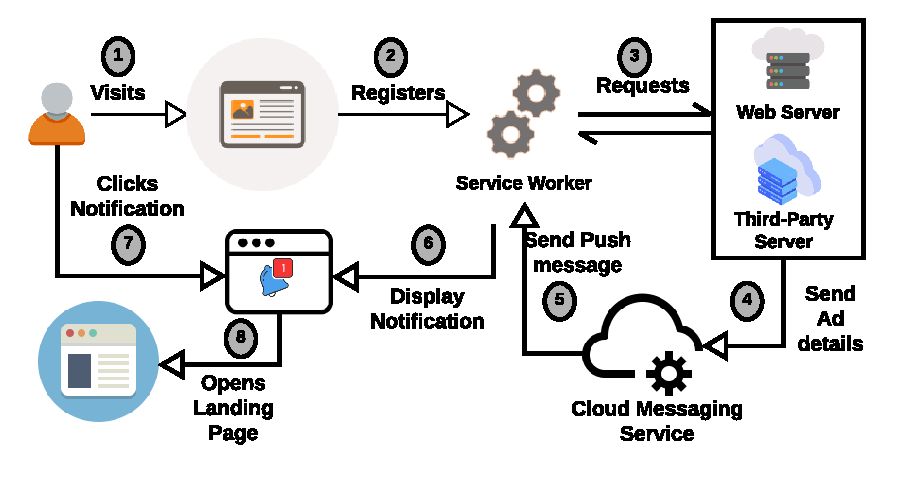
\includegraphics[width=\columnwidth]{figs/service_worker.pdf}
\caption{Steps involved in Serving Ads via WPNs}
\label{notification_system}
\end{figure}



\noindent \textbf{Service Workers and Push Notifications:} A Service Worker is basically a javascript file that runs in the background with a context different from a web page process. For a service worker to be installed and running, a user has to visit a web page that provides a link to the service worker javascript file. A service worker registers itself as long as the web page that it was downloaded to was served via HTTPS. A service worker plays multiple roles when it comes to different functionalities such as offline loading, background processing and pushing web notifications. Since this paper focuses on WPNs, we limit our explanation of service worker to it's role in WPNs. Once a service worker is registered, to subscribe to WPN, it needs to check if the website has permission from user to send notification. A subscription is made by exchanging keys that can be used to validate the sender and receiver of the push notifications. On visiting multiple Progressive Web Apps(WPA), multiple service workers gets registered on the device. Further, a single PWA is allowed to register multiple service workers as well. Therefore, the subscription helps create a mapping between the service worker and the ad server that is authorized to send notifications to it. After subscribing to WPNs, the role of service worker is to listen to any push messages sent for it to display and it does so by using a listener to \texttt{OnPush} event. At this point, service worker uses the \texttt{ShowNotification} event of \texttt{Notification} API to display the push message as a web notification. The notification has certain customizable parameters such as title, body, target URL, icon image, display image and action buttons. The user can then interact with the shown notification by either clicking on it, closing it or performing any custom actions that are shown in the notification. The service worker can choose to listen to any such user events and act accordingly. A service worker can make requests to fetch resources from any server or to send reports on the click events to any server. Usually, a service worker once registered will continue to exist in the user's machine unless they are explicitly unregistered. A step by step illustration of serving ads via WPNs is shown in Fig.\ref{notification_system}.   

\noindent \textbf{Firebase Cloud Messaging(FCM):} FCM is a cross-platform messaging solution for Web based Push Notifications. It serves as a central authority mediating the communications between the ad server and  the service worker. At the subscription stage, FCM creates a unique registration id per user per service worker and this is sent along with an endpoint to the ad server. Whenever an ad server wishes to send a notification to its subscribed user, it makes a request to FCM server along with the endpoint. FCM authenticates the sender using the keys that were exchanged earlier and it is using this endpoint that FCM understands which user machine and browser it has to deliver the notification. \warn{Should I explain the difference in receiving push messages between desktop and mobile here? It is explained later in system design}   

\noindent \textbf{JSGraph:} JSGraph by Bo Li et al. \ref{jsgraph} is a forensic engine that enables logging of  JavaScript(JS) executions and JS- driven DOM modifications within the browser at a fine-grained level. JSGraph is implemented by instrumenting Chromium code base and thus makes it portable to different platforms and browsers that support Blink/V8 engine. With the help of JSGraph, we can record all changes to the DOM, monitor navigation events, record execution details about Javascript code and changes to the DOM that are made by the Javascript code. Since Javascript plays a major role in advertising, we need a clear understanding of the scripts involved in advertisements and their effects. Any more changes required to suit our needs could be done by following a similar procedure of modifying Chromium code base. Moreover, the overhead caused by the instrumentation is acceptable thus making it a suitable tool for us to develop our system.

\noindent \textbf{Puppeteer:} Puppeteer is a NodeJS library that allows us to automatically control Chromium or Chrome over headless or non-headless mode. Since this is a tool developed by Google Chrome, it provides support to most features of Chromium and the code can be customized to suit our needs. This tool provides us with high level API useful to perform actions such as open window, navigate to a page,record network requests and responses, perform events such as click, scroll and select, capture screenshots and monitor multiple tabs. In our project, Puppeteer tool is also used to monitor events related to service workers and any requests made by the service worker. To achieve this, we found a service worker module of puppeteer that is still under development and use its features.

% With introduction of smart phones and development of their software development kits, very soon delivering information to the smart phone through push notifications became a dominant feature in apps. Push notifications allowed delivery of updates and content to apps in a resource aware manner. This meant the applications did not need to be always active draining power and processing resource, and yet, they were able to receive updates. 
% It was only recently that such long awaited feature was introduced for the web world as Web Push Notification-WPN-. Web push notifications in general contain three major components, a requester that provides the content, a relay server which receives the content and distributes them among the users and a subscriber code running on target devices which stands by -usually in the background- to receive the notifications. WPNs differ from push notifications delivered to mobile applications by the fact that WPNs do not require any installed code through the applications, they are cross platform and they are handled by the browsers not other applications. 

% In Google Chrome WPNs rely on \textit{service workers}. Service workers allow web sites to spin off a background process. once registered, this back ground process will stay active even when user is not interacting with the page directly and are majorly used for receiving WPN or syncing in the background. 
% To receive WPN in Google Chrome, a web site has to first be granted push notification permission, then it will launch a service worker and register the device with the push provider. Service worker will wait on new content to be delivered from push provider, then based on the content or the metadata in the pushed object then, service worker will decide its logic which might include showing a popup message or syncing and updating a piece of data. 





\section{Motivation}
Over the last few years, the advertisement industry has been constantly evolving to stay in par with its user base. The increase in number of mobile users and user tracking technologies allow advertisers to serve ads in a more efficient manner. One such trending change is the advertisers and website owners opting to serve ads through Web Push Notifications(WPNs) on mobile and desktop. Megapush is one of the first ad networks to start serving ads through WPNs and currently it has over 450 million subscribers. The main reason for ad networks to prefer WPNs over traditional online ads is that delivery won't be curbed by third party ad blockers. Unfortunately, delivering ads through WPNs open a wide arena for scammers to reach large number of potential victims as well. During our initial stages of research, we had visited a website \texttt{https://aurolog.ru}. When it requested for notification permission, we granted permission by pressing the allow button on the browser dialog box. Please refer Fig.\ref{tech_scam} for a visual representation of the case. Next, we had received an ad with an alert message 'Your payment info has been leaked'. When we proceed and click the notification, we were redirected to a tech support scam web page, as shown in Fig.\ref{tech_scam}. To our surprise, the landing URL was not blacklisted by Google Safe Browsing or detected as malicious by Virus Total. This made us wonder how many more such cases exist and how else are the advertisers utilizing WPN ads. In order to better understand the push advertising ecosystem and it's reach in the real world, we develop a system  \sysname that automatically subscribes to push notification ads, interacts with the ads and tracks any information related to the notification service.Although the discussed example is a malicious one, we do not limit our focus to finding only malicious advertisements. Using our system \sysname, we were able to successfully track over 7000 advertisements delivered through push notifications. 

\begin{figure*}[ht]
\begin{center}
\includegraphics[scale=0.07]{figs/tech_scam.pdf}
\caption{Example of malicious advertisement served through push notification}
\label{tech_scam}
\end{center}
\end{figure*}

The major goal of our system is to perform a study on the existing push advertising ecosystem. To begin with, we need to ensure the following requirements to achieve our goal.

\begin{itemize}
    \item Effectively collect a detailed log of events that happen during multiple stages of Web Push Notification
    \item To a full extent, automate all user actions that are required during these multiple stages
    \item Design a system that can be scaled and ported to any web platform
    \item Perform analysis on advertisements offered by all Web Push Ad networks irrespective of their popularity
    \item Design a systematic way to analyze large amounts of data and perform an extensive study on the data collected to provide measurements related to push advertising ecosystem 
    \item Ensure that the system can be implemented in desktop and mobile environment thus providing us insight on push advertising in both environments. 
\end{itemize}







\section{System Design}
\sysname is a framework to trace advertisements that are delivered through push notification service to the end users. In this section we explain the design of \sysname and it's various componenets.

\subsection{Overview}
Multiple steps are required for a website to get an end user to subscribe to its notification service and display an ad through push notifications. It has to be noted that some of these steps mandate user interaction and requires user permission and poses as a major challenge to automate the entire process. As of now, no framework exists that allow the automation of successfully interacting with a push notification process. Therefore, we extend the chromium module of a forensic engine, JSgraph\ref{jsgraph} to suit our needs. \sysname record essential information involved at each step and automates actions that are required to successfully proceed from one step to the next. In order to record necessary information, we need a complete trace of events that happen in a chromium browser from visiting a chosen website to receiving a notification from the website and interacting with the notification. We achieve that by leveraging the modified chromium module used in JSgraph\ref{jsgraph}. As major part of our system involves chromium browser and it could be deployed in both desktop and mobile environment, We develop additional modules that would help us launch and automate interactions with chromium browser for both desktop and mobile environment. Various steps involved in the notification service of a chromium browser are shown in \ref{notification_system} and the role of \sysname at each step is explained in detail for desktop and mobile environment in the following sections.


\subsection{Desktop Environment}

\subsubsection{Handling Permission Request}
A website requires the user's permission to send push notifications. When the user visits a website, the website conveys it's intent to send a push notification to the browser. Then, the browser displays a browser dialog box to request permission from the user. To automate this process, \sysname logs the request made by the website to the browser at \texttt{RequestPermission} method of \texttt{PermissionContextBase} module in Chromium. %To mimic user's behaviour of granting permission to notifications,
We modified the \texttt{PermissionDecided} method of \texttt{PermissionContextBase} module to grant permission by default and also record the permission's status. Thus, notification permission requests from any website that \sysname visits will be granted permission automatically.


\subsubsection{Handling Service Workers}
A service worker~\cite{chrome_service_worker} plays a vital role to register, deliver, and display notification. Fig.~\ref{notification_system} illustrates the overview of the push notification service in Chromium. Service workers perform important processes including registration of the push notification (step 2), handling notification requests (step 3), sending push messages (step 5), and displaying the notification (step 6). Furthermore, service worker also play a role to open a website (i.e., landing page) if the user clicks the notification (step 7). We explain in details how service workers serve push notifications and the information we record at each step.

\textbf{\indent{Registration (step 2): }}
Any website can register a service worker script without user authentication it satisfies certain criteria~\cite{chrome_serviceworker}. We instrument \texttt{ServiceWorkerContainer} module in Chromium to hook \texttt{register} event that allows us to log registration of each service worker. The information we log is including the URL of the service worker and the website origin that registered the service worker. Once the service worker registered, it can subscribe for push messaging service of the browser. During this subscription, an application server key is passed to the browser to identify the app server via Google Firebase Cloud Messaging (FCM)~\cite{google_fcm}. This key denotes the party responsible for sending push messages. Hence, we record the key information at \texttt{subscribe} method of \texttt{pushmanager} module in Chromium.  At this point, the status of service worker is active and ready.

\textbf{\indent{Requests (step 3): }}
After a service worker is activated, it can send push notification requests to any server, including web-server that the user visited or a third-party advertising network.
%The third-party servers could vary from any ad network servers that are responsible for serving ads to a server that tracks certain measurements at regular interval. 
These requests made by service workers are outside the context of the webpage, and thus, we need to record them at the service worker context. We instrument the service worker module to hook \texttt{request} event. It allows us to log all push notification request events from each service worker when they are registered using \texttt{Puppeteer} tool. \KYU{What is puppeteer tool? Please explain it.} Also, we hook \texttt{response} event in a similar fashion. The information collected related to the requests and responses are \texttt{request-origin},  \texttt{request-url}, \texttt{post-data}, \texttt{redirections} and \texttt{response-content}. The response content is recorded in the log file for further analysis.


\textbf{\indent{Handling Push Messages and Notification (steps 5\&6): }}
The browser receives push message from the cloud messaging service and alerts the service worker that is responsible to receive the content. Each service worker has a unique identifier which is specified in the push message. Then, the service worker receives the push message by listening to \texttt{push} event and invokes the \texttt{showNotification} method of \texttt{ServiceWorkerRegistrationNotifications} module in chromium by passing the necessary data. However, it is not mandatory for a service worker to invoke \texttt{showNotification} method. In such case, the chrome browser would still by default display a notification by invoking the same method. Hence, we record the data at \texttt{showNotification} method by invoking the \texttt{WillShowNotification} method of \texttt{Forensics} module. The data collected includes \texttt{service worker URL}, \texttt{notification title}, \texttt{notification body}, \texttt{notification image URL} and \texttt{notification target URL}. Further, whenever a request is made by the service worker as mentioned in step 3, a screenshot of the entire desktop is captured. AS, a service worker is bound to make a request for an image to display for notification, capturing a screenshot after a short delay of each request helps us capture the notification that is displayed by the browser.


\textbf{\indent{Handling User Interaction with Notification (steps 7\&8): }}
When a user clicks a displayed notification, the service worker could listen to click event and it could either do nothing or navigate the user to a web page. We wanted to record this observation for further analysis. However, the challenges at this stage include emulating an user click once a notification is displayed and recording the events that occur once the click happens. First, to emulate an user's click, since the notification itself is on a different context than the web page, the automation tool \texttt{Puppeteer} cannot be used to emulate a click. However, in the chromium environment, the method \texttt{Add} of \texttt{MessageCenterNotificationManager} module is responsible for generating the notification. Also, the \texttt{Click} method of \texttt{WebNotificationDelegate} triggers a click on the notification. Therefore, we modified the \texttt{MessageCenterNotificationManager.Add} method to invoke \texttt{WebNotificationDelegate.Click} after a delay of 10 seconds. The delay is meant to provide enough time to capture a screenshot of the notification. Second, if the click results in a navigation to a web page, the modified chromium as mentioned in JSgraph \ref{jsgraph} records all redirection and fine-grained details of the page and its execution. At this stage, a service worker may listen to click and close events of notification shown and contact a server to report this information.

\subsection{Mobile Environment}
For mobile environment, we devise our system to work on a real android device. We compile the altered Chromium code for Android device. Certain steps that are involved in the push notification service work differently in a mobile environment. Firstly, while handling user interaction with notification (steps 7 \& 8), desktop environment requires the Chromium process to be running in order to display the push message sent by any website. However, In Android device, mobile operating system will generate the notification pop-up for user as a system notification and the application (Chromium) itself is not activated until someone clicks on the notification. In desktop environment, we used Puppeteer framework to automatically interact with the chromium browser to browser URLs. On the other hand, in Mobile, we use Android Debug Bridge (ADB) to start the chromium browser and enter URL into the browser. Since a service worker spawns as a different process than chrome, the requests (step 3) made by service worker script are not logged by the chromium browser itself and is not collected in mobile environment. Different components involved in mobile environment are explained below. 

\textbf{\indent{Enabling Notification Click: }}
In order to simulate user behavior to interact with the notifications, we developed an Android application that leverages the Android accessibility service. The accessibility service is aimed to help people with disabilities in using the device and apps in it. It is a long-run privileged system service that helps users process information from the screen and lets them interact with the content meaningfully in an easier way. An android developer can leverage the accessibility service API and develop apps that are made aware of certain events such as \texttt{TYPE\_VIEW\_FOCUSED} and \texttt{TYPE\_NOTIFICATION\_STATE\_CHANGED}. Further, it could also be used to initiate user actions such as click, touch and swipe. Our application that is pre-installed on the device has the permission of accessibility service and monitors every notification event fired from Chromium. Whenever a new notification pops up, our application will automatically swipe down the notification bar and click on the notification to complete the action. 

\textbf{\indent{Generating Event Logs: }}
The modified chromium code that logs events related to notification service along with the logs generated by the JSGraph\ref{jsgraph} version are the same for desktop and mobile browser. We built and compiled the same code for Android setup. However, the logs are generated in a different manner. The logs generated from every application in the device is collected by using the \texttt{logcat} command in ADB tool and piped into a destination file. \texttt{logcat} is a developer tool letting the developers print messages for debugging purpose. All the logs of chromium from different tabs, in addition to all the logs from other applications are piped into a single log file. We then later translate this file into desktop-version logs with only chromium logs. In this case, we can use one parser to analyze both desktop and mobile logs. Although the logs from different websites are mixed in one log file, we still can use post-analysis to successfully separate logs from each website.





\section{Experiment Setup}
This sections explains in detail the data collection stage and system setup.

\subsection{Seed Domain Collection}
During the data collection stage, we focused on collecting domains that serve advertisements via push notifications. Therefore, to start with, we manually browsed Google for a list of ad networks that are known to serve ads via push notifications. Then, we manually signed up as a publisher with each of these ad networks to obtain the script code that needs to be added to a website to enable the ad network's service. Later, we formed a list of certain keywords from each script that uniquely points to their associated ad network. We then use the keywords to obtain a list of domains that possibly use the ad network that the script belongs to. We searched for domains that contains keywords pointing to an ad network by using the service of source code engine, \texttt{publicwww.com} \ref{publicwww}. At this point, we had a list of 1,75,939 domains to start our analysis and the distribution of domains along with the seed keyword used to obtain them is shown in table \ref{seedDomains}.


\begin{table}[htbp]
\caption{Seed Domain Details }
\begin{center}
\label{seedDomains}
\begin{tabular}{c|c|c|c}
\toprule
\hline
\multirow{4}*{\textbf{Ad Network/Seed Keyword}} & \multicolumn{3}{c}{\textbf{Domains Count}} \\ 
\cline{2-4}
~ & \textbf{HTTPS} & \textbf{HTTP} & \textbf{\makecell{HTTPS \\Notification \\Permission}}\\
\hline
 \hline
 cloudfrontnet & 49769 & 50148 & 1394
 \\
 \hline
 cdnpushcrewcomjs & 15177 & 5143 & 478
 \\
 \hline
 cdnonesignalcomsdk & 11317 & 7241 & 3149
 \\ 
 \hline
 NotificationrequestPermission & 3965 & 6417 & 562
 \\ 
 \hline
 pushmanagersubscribe & 2667 & 800 & 173
 \\ 
 \hline
 popadsnet & 1581 & 8154 & 80
 \\ 
 \hline
 apipushengagecom & 796 & 896 & 238
 \\ 
 \hline
 cdnizootocomscripts & 676 & 625 & 301
 \\ 
 \hline
 pubmaticcomAdServer & 647 & 230 & 8
 \\ 
 \hline
 adnetworkpropellerads & 335 & 740 & 10
 \\ 
 \hline
 addEventListenerpush & 250 & 43 & 9
 \\ 
 \hline
 criteocomdeliveryajsphp & 154 & 1540 & 5
 \\ 
  \hline
 terraclickscom & 86 & 662 & 0
 \\ 
  \hline
 adsblockkpushcom & 55 & 4235 & 21
 \\ 
  \hline
 airpush & 52 & 169 & 0
 \\ 
  \hline
 puservingcom & 29 & 628 & 2
 \\ 
   \hline
 hilltopadsnet & 21 & 160 & 3
 \\  
   \hline
 adsad4gamecomwww & 14 & 179 & 0
 \\   \hline
 richpush & 12 & 10 & 0
 \\   \hline
 adcashcomscriptjava & 10 & 258 & 0
 \\   \hline
 jspushmonetizationcom & 9 & 14 & 5
 \\ 
 \hline
 \bottomrule
    \end{tabular}
\label{tab1}
\end{center}
\end{table}

\subsection{Filtering Seed Domains}
As a first stage of processing, we filtered the list of seed domains collected to retain only those that request for notification permission. To achieve this, we visited each of the seed domains using our framework \sysname. The log generated by the Chromium component records any request for notification permission. Thus, we parse the logs to check if a request to notification permission was made. Only those domains that request to send notifications to users are retained for the next stage of processing. The number of domains that requests notification permission is shown in table \ref{seedDomains}

\subsection{Monitoring Notifications : Desktop Environment}
In desktop environment of \sysname, we use docker containers  to monitor notifications. For each domain that has to be monitored, a docker container is created to provide a virtual environment. As we create separate containers for each domain, it prevents ad networks from fingerprinting the user using any third party cookies and other user based information. Further, it also allows us to visit multiple domains in parallel increasing the rate of our experiment. Since we already filtered the domains that request for notification, we proceed with the monitoring phase as follows

\begin{itemize}
    \item First, we create a new docker container for each domain that needs to be monitored. This docker container already has the modified Chromium installed in it. 
    \item We execute a nodejs script that uses puppeteer tool to automatically control the Chromium browser in each container. This script starts Chromium browser and opens the website URL that is passed to it on a new tab. By default, service worker  gets registered and Chromium grants permission for notification to the website. In order to allow time for the website to load, register it's service worker and request permission, the web page is kept open for until 5 minutes. 
    \item At this point, after the service worker is registers, the docker container is kept alive for 15 minutes. In a desktop environment, for Chromium browser to receive push messages, the browser process needs to be running. Hence, even though we close the web page after 5 minutes, we keep the browser process running. It is essential to close the web page after 5 minutes because, it is possible that the website won't send any notification as long as the web page is open.
    \item After 15 minutes of monitoring the docker container, we stop the container and proceed with monitoring next URLs. Stopping the container frees both CPU and memory used by the container and its process. However, the container could be started at any point of time to resume the operation.
    \item After a certain period of time, we resume the stopped container and execute the nodejs script to open the browser process. Since this browser process uses the same user profile, the permission provided previously applies to this session. However, service workers are designed to become inactive after a certain period of time. Service workers are activated whenever a push message is sent to them. Therefore, whenever a push message is sent by the messaging server, the service worker is activated and it continues with the process of displaying notifications.
    \item Whenever we resume a container and start the browser process, it tends to display all the queued notifications 3 at a time. But all these queued notifications would be added at the same time as soon as the browser is active. Since, our system is designed to emulate a click 15 seconds after it gets added, some notifications might be clicked even before they get displayed. To resolve this issue, we modified Chromium code to induce a delay of 10seconds whenever it adds a notification using the \texttt{MessageCenterNotificationManager.Add} module. This ensures that all queued notifications are displayed before a click is emulated.
    \item A resumed container is kept open for 15 minutes and stopped to be resumed at a later point of time. This helps to mimic an user's behavior of closing the browser or staying logged off for specific duration in a day. Also, this allow us to efficiently utilize the system resources to monitor next set of URLs. 
    \item The executed nodejs script and the modified Chromium records every interaction as mentioned in system overview. This includes capturing a screenshot of every web page that opens and the notifications that get displayed. The logs collected through the script and Chromium tool provide us a fine-grained detail of the execution of web page and the service worker involved. 
\end{itemize}

%%%%%%%%%%%%%%%%%%%%%%%%%%%%%%%%%%%%%%%%%%%%%%%%%%%%%%%%%%%%%%%%%%%
\subsection{Monitoring Notifications: Mobile Environment} \label{monitoring}
In mobile environment of \sysname, We had to take into consideration the device's physical and technical limitations. \st{In order to collect website notifications from mobile environment, there are two ways that we took into consideration.}\samuel{The reasons we are collecting website notifications from a real mobile device are because} 1) To use the feature in desktop Chromium that could change the view to a mobile view to collect ads in mobile environment. \samuel{Website can easily detect whether the environment is mobile or not(citations). And based on our observation, advertisement network would send out mobile-specific advertisements to attract uses' attention. } 2) Since most of the websites now use advanced tracking methods to determine if a mobile user is legit by monitoring various sensors such as acceleration, orientation, location etc., \samuel{In order to lower the risk of losing notifications, }we chose \st{the later option} to run experiments on a real android device. Also, in android devices sometimes, they look for google play services which could not be simulated using a \warn{Chromium mobile view}(\samuel{This term is not easy to understand I think}). 

\samuel{However in mobile environment of \sysname, We had to take into consideration the device's physical and technical limitations. 
 Certain physical features of a mobile device such as memory and CPU processing restrict the number of URLs that we could monitor over a period of time compared to desktop setup. In order to collect notification in an efficient way, we open multiple URLs in one chromium application. Even though the logs are mixed in one log file, we still can separate logs from different websites later using the parser. We use a Nexus 5 running AOSP(Android Open Source Project) version 7.1.1\_r38 with Open GApps\cite{gapps} installed.} The procedure followed in collecting notifications on a mobile device are listed below.   
\begin{enumerate}
    \item First, we install modified Chromium and our app on the device using the command below. \samuel{The parameter \texttt{-g} is to grant chromium all the application level permissions it might ask for later. There are two levels of permissions in chromium. First is application level permissions, which are controlled by Android Operating System. Second is website level permissions, which are managed by chromium. The application level permissions are shared within all the websites inside chromium. However, chromium still would ask for user's consent for website level permission if the website is asking for sensitive information, like in fig. \ref{website_level_permission}. We granted the application level permissions during installing time of chromium \warn{ and granted website level permissions through modifying chromium source code}. \\
        \texttt{adb install -g MonochromePublic.apk}}
    \item Next, we create a custom browser setting profile and push it into the device using ADB. In the setting profile, we turn off third party cookies, safe browsing, data saver, and other options that might interfere the data collection. As we cannot sandbox each URL's visit in a mobile environment, turning off third party cookies would prevent same ad network used by different domains \st{that we visit} to fingerprint the user. Once an ad network fingerprints the mobile device as a single user, it might hinder the number of ads that are delivered to the device by the ad network. \st{Further,}Google's safe browsing might block websites that are on our list if it deems them malicious and this would limit our domain pool. On data saver mode(renamed lite mode in recent releases), some of the web traffic may go through Google servers before reaching the device. We turned off this option in case Google servers have safety mechanism to block malicious websites\samuel{, or in some cases, Google may modify/compress the website's source code in order to make it faster to load. }.
    \item \label{spawn_website} Then, we connect the device to a computer in order to control the device using ADB. We use the following ADB command on the connected computer to start Chromium and visit a domain on the device. 
        \texttt{adb shell am start -n \path{org.chromium.chrome/org.chromium.chrome.browser.ChromeTabbedActivity} -d [URL] --es \path{"com.android.browser.application_id"} "com.package.name"}
    \item At this point, logs printed to \texttt{logcat} from Chromium app are piped into our log file. At the same time, we are monitoring the CPU load using the following command.\\
        \samuel{\texttt{adb shell uptime}}
    \item After visiting a page, we waited for 5 minutes to allow for the website to load, successfully register service worker and gain permission to request notification. This time interval was determined based on our observations that is shown in Fig. \ref{sw_reg_time}. 
    \item After 5 minutes, we proceed with visiting next URL on a new page using the command in Step \ref{spawn_website}. Any service workers that were registered by previously visited sites would be running in the background.
    \item After we open all the pages, we wait for 5 days to receive notifications. 
\end{enumerate}

\begin{figure}[h]
\begin{center}
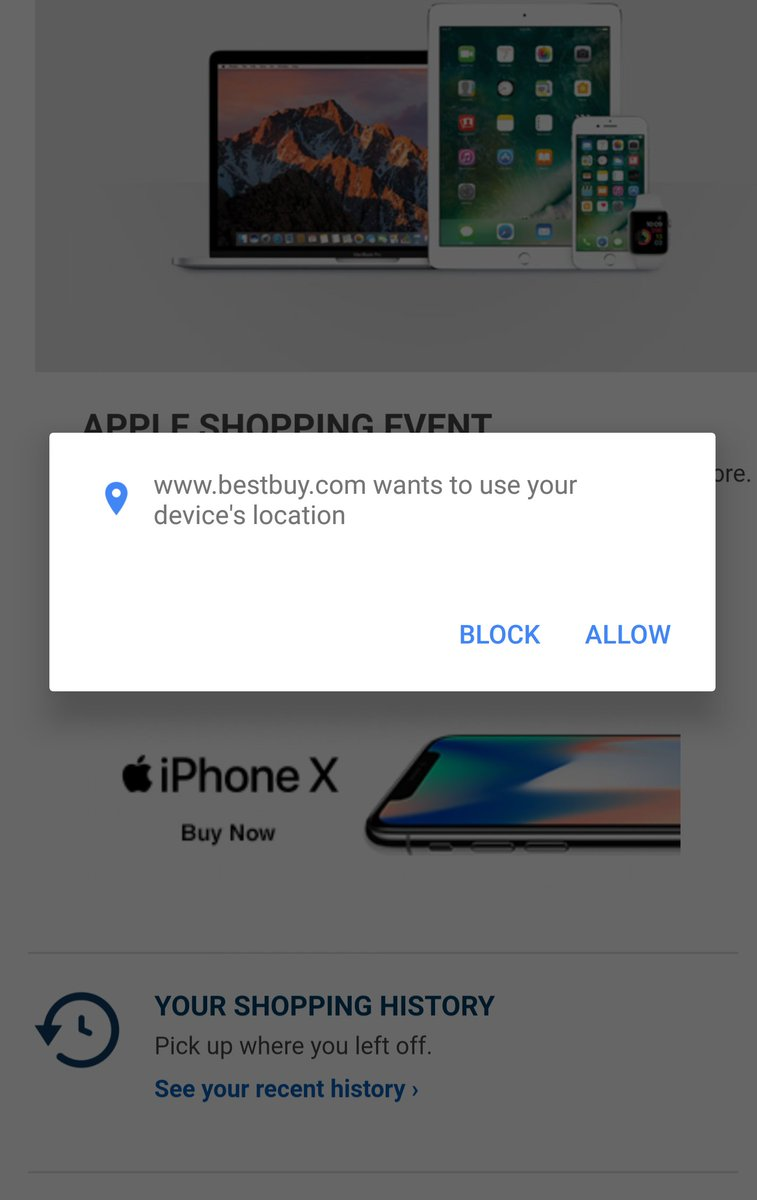
\includegraphics[scale=0.25]{figs/website_level_permission.jpg}
\caption{Example of website level permission on mobile device.}
\label{website_level_permission}
\end{center}
\end{figure}

At any point during this experiment, the mobile device can run out of battery as it is only charged through the USB connected to the computer \samuel{(approximately 0.5A/5V)} that controls the device using ADB. Under such circumstances, our experiments would be stopped abruptly. In order to overcome this problem, we monitor the device's battery level and when it is below a certain level \samuel{we pause the android device using \\\texttt{adb shell stop}\\ and resume it once the device is fully charged using \\\texttt{adb shell start}\\ The advantage of using these commands is we can still using ADB to monitor the device battery information while the essential components, including Zygote(core process of Android applications), SystemServer and SurfaceFlinger(display)\cite{android_graphics}, are stopped.} Once resumed, the processes continue with their operations as though there was no delay involved. \warn{Although the previous notifications are cleared out. But I guess we don't need to mentioned them... or do we?}

\subsection{Parsing Logs: Desktop Environment}
After we run the experiments, we obtain a chromium log file for every docker container session. This log generated by Chromium is very detailed as they contain fine-grained information about all DOM modifications, Notification related calls and events, critical JS
API calls and parameters etc. Therefore, we parse the log file to filter out any redirection, service worker registration, subscription keys,notification permission request, notification events such as show, click and close, API calls made by service worker and tab open. We record the filtered log entries and attributes related to each entry in a database. Note that the log generated from a single docker session may have information about multiple websites. For example, If we initially visit a website ABC.com and after clicking the notification received from ABC.com, we were redirected to XYZ.com and XYZ.com also has a notification service, then our log would contain the information for both ABC.com and XYZ.com. Additionally, in desktop environment, we save any resources that are requested by the service worker such as javascript files, image files etc. We parse these resource files to fetch any URLs that are found in them and also calculate the hash of files and store them in the database for further analysis.


\subsection{Parsing Logs: Mobile Environment}
\samuel{I think we can say mobile and Desktop are basically using the same parser. That's the beauty of our tools, right?}
\section{Analysis Results}
In this section, we describe the application of our system, \sysname on real world to gather information on the working of service workers and it's role in notification service. We calculate measurements that help us understand the advertising ecology and their behaviour. We use the filtered URLs that requested for notification permission and monitor these URLs as mentioned in \ref{monitoring}. We have collected data over multiple periods of time while making any improvements that are required to the system based on the data observed previously. 

\subsection{Notifications in the Wild}
From the logs collected over a initial set of URLs, we were able to obtain the time taken by websites to request for notification permission and it is shown in fig.\ref{req_time}. We could observe from this figure that over 95 percent of the websites took under 3 minutes to request notification. Hence, of the 3000 websites that were used for this measurement, 2850 websites requested permission under 3 minutes. This helped us to decide on the wait time of 5 minutes for which we keep a website open on the browser while visiting the website for the first time. The 5 minutes wait time also takes into consideration any delay caused in loading the website. 

\begin{figure}[h]
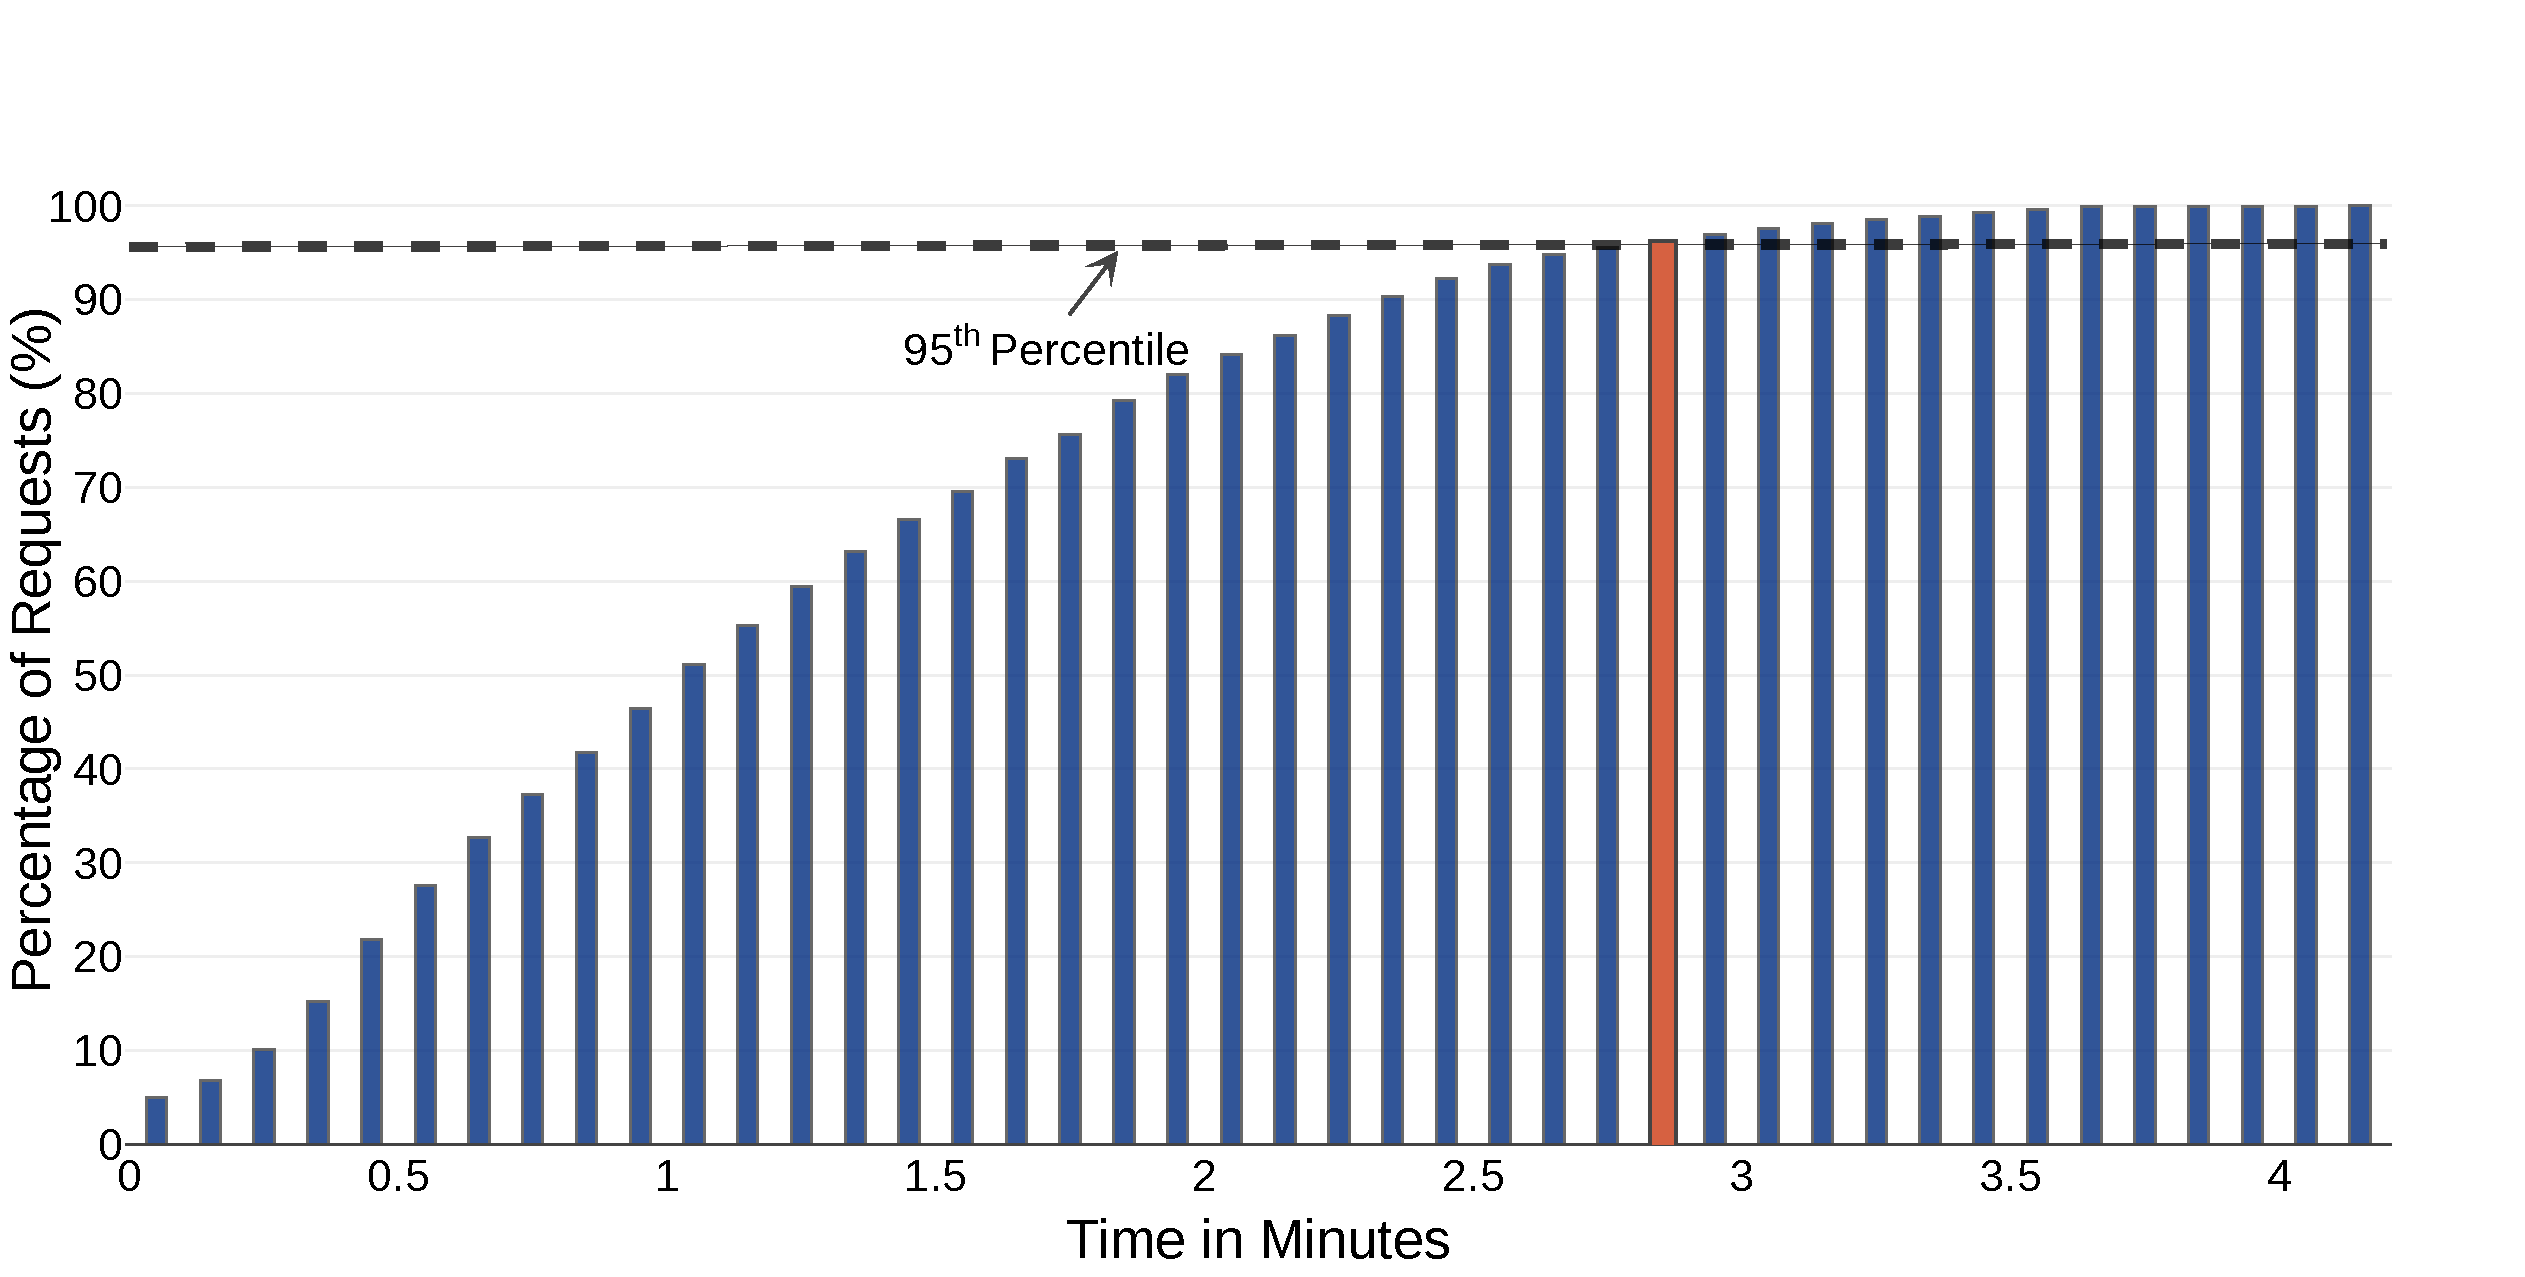
\includegraphics[width=\columnwidth]{figs/req_time.pdf}
\caption{CDF of time taken by sites to request permission. The number of requests made by websites are shown in percentage in y axis. }
\label{req_time}
\end{figure}

Next, We obtain the time it takes for a website to send it's first notification and we collect this measure from multiple websites that we monitored and the result is shown in fig.(\samuel{There's a string macro called \figurename. You might want to use that?}) \ref{first_notification}. This measure helped us decide the duration for which a docker session in desktop environment should be kept active. Next, we measure the count of notifications sent by a website to the end user per day. The results are quite alarming and a vast difference between mobile and desktop environment can be observed. We count the number of notifications sent by a service worker per day and calculate minimum, maximum and average number of notifications over multiple days and plot them in a graph as portrayed in fig. \ref{notification_per_day}. We had 506 and 303 service workers from desktop environment and mobile environment respectively. The maximum number of notifications sent by a service worker turned out to be \textbf{90} and \textbf{316} for desktop and mobile respectively. Around 12\% and 20\% of the service workers have sent over 10 notifications on an average per day in desktop and mobile environment respectively. It can be observed from these numbers that mobile users are targeted and preferred more by malicious ad networks.

\begin{figure}[h]
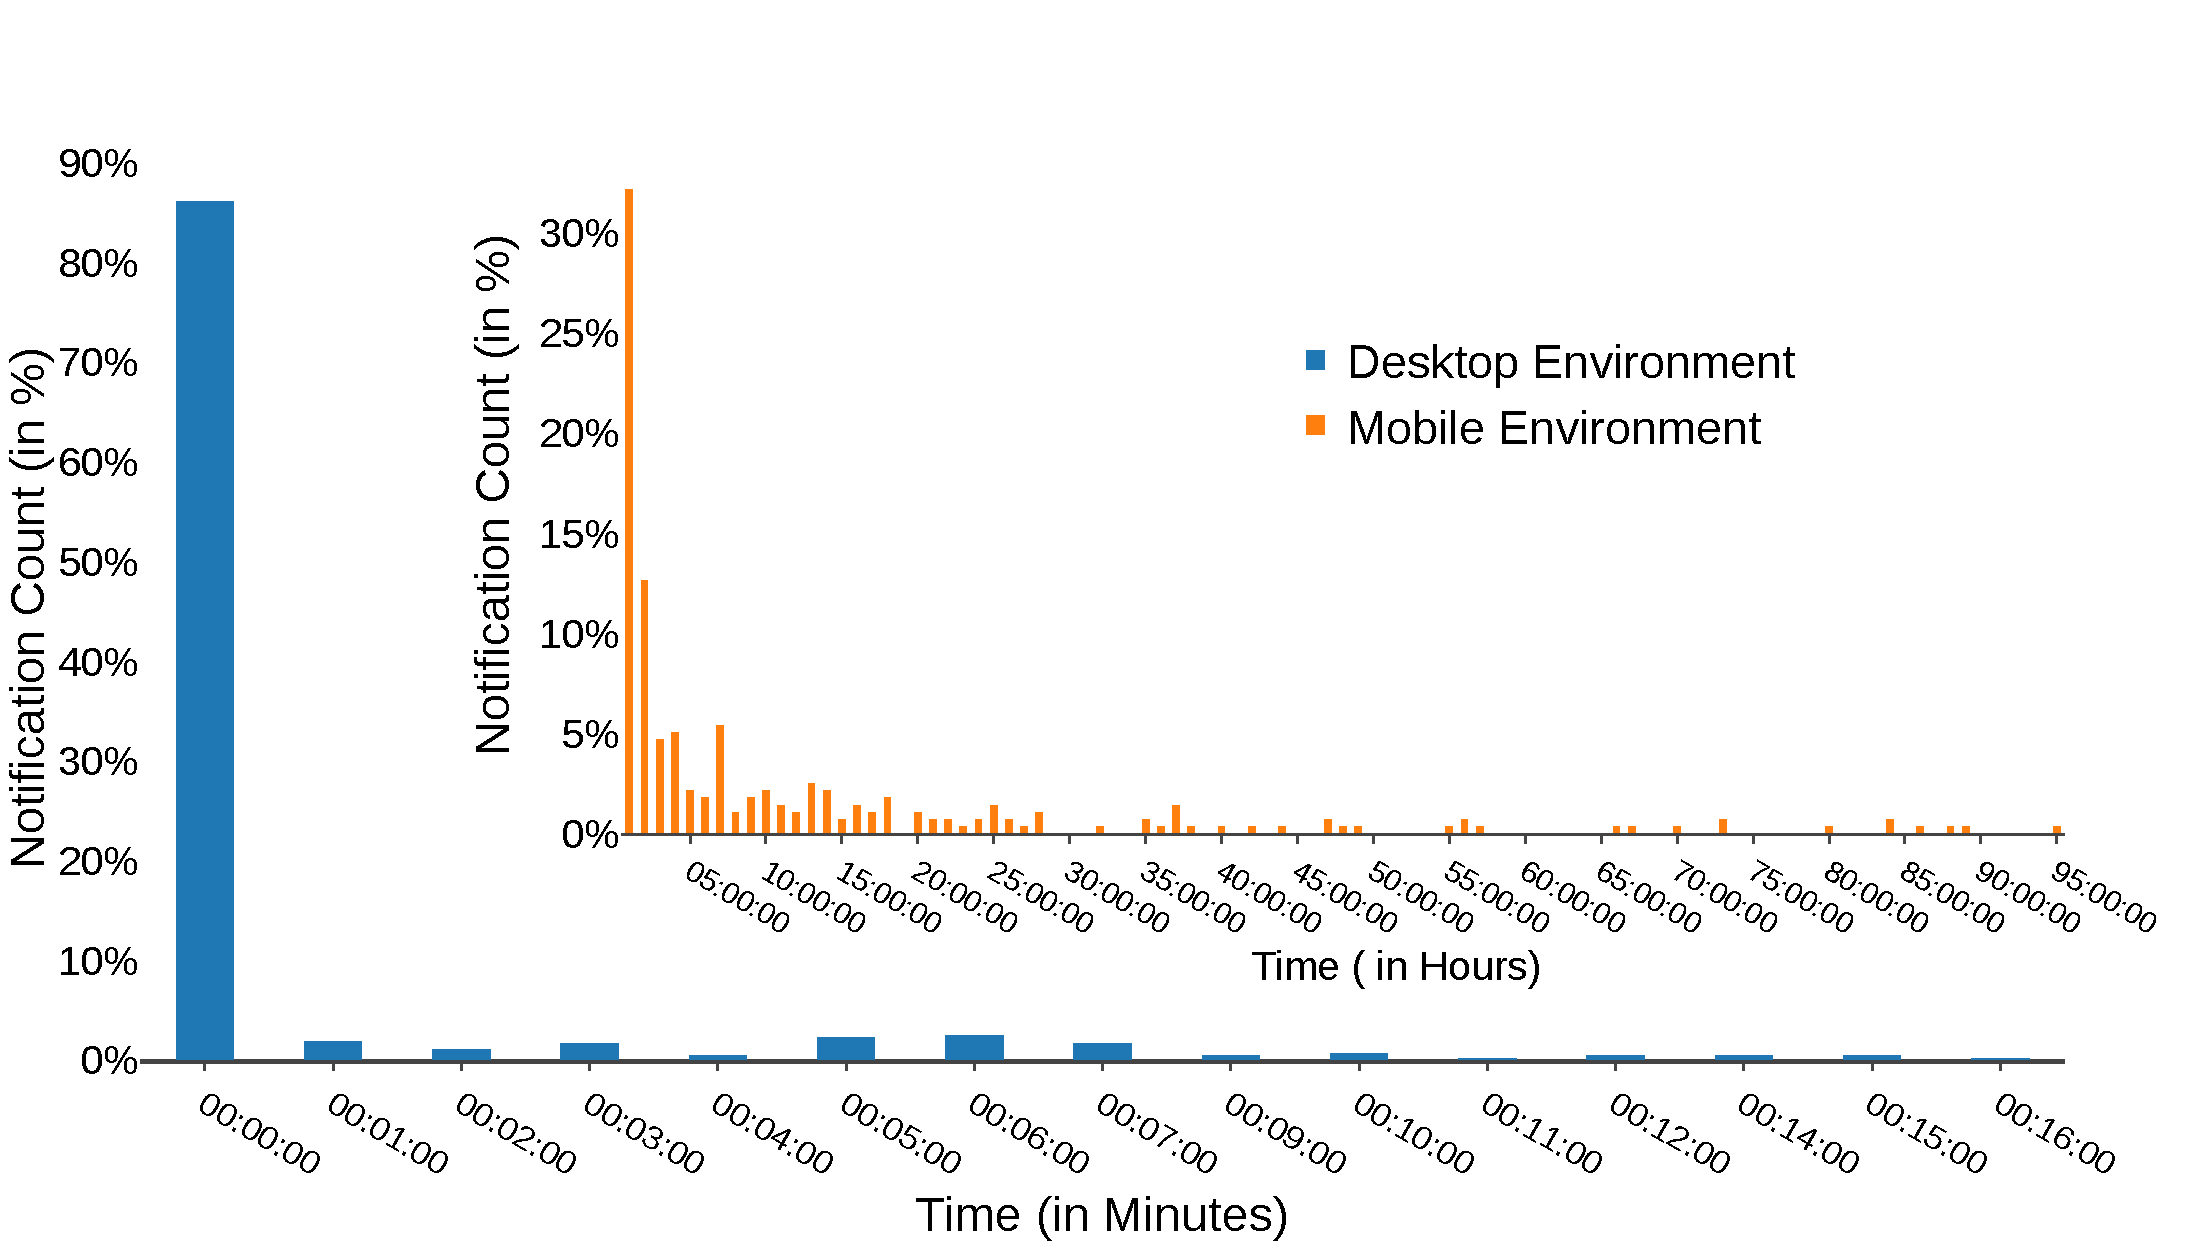
\includegraphics[width=\columnwidth]{figs/first_notification_histo.pdf}
\caption{Time taken for websites to send their first notification}
\label{first_notification}
\end{figure}

% \begin{figure}[h]
% 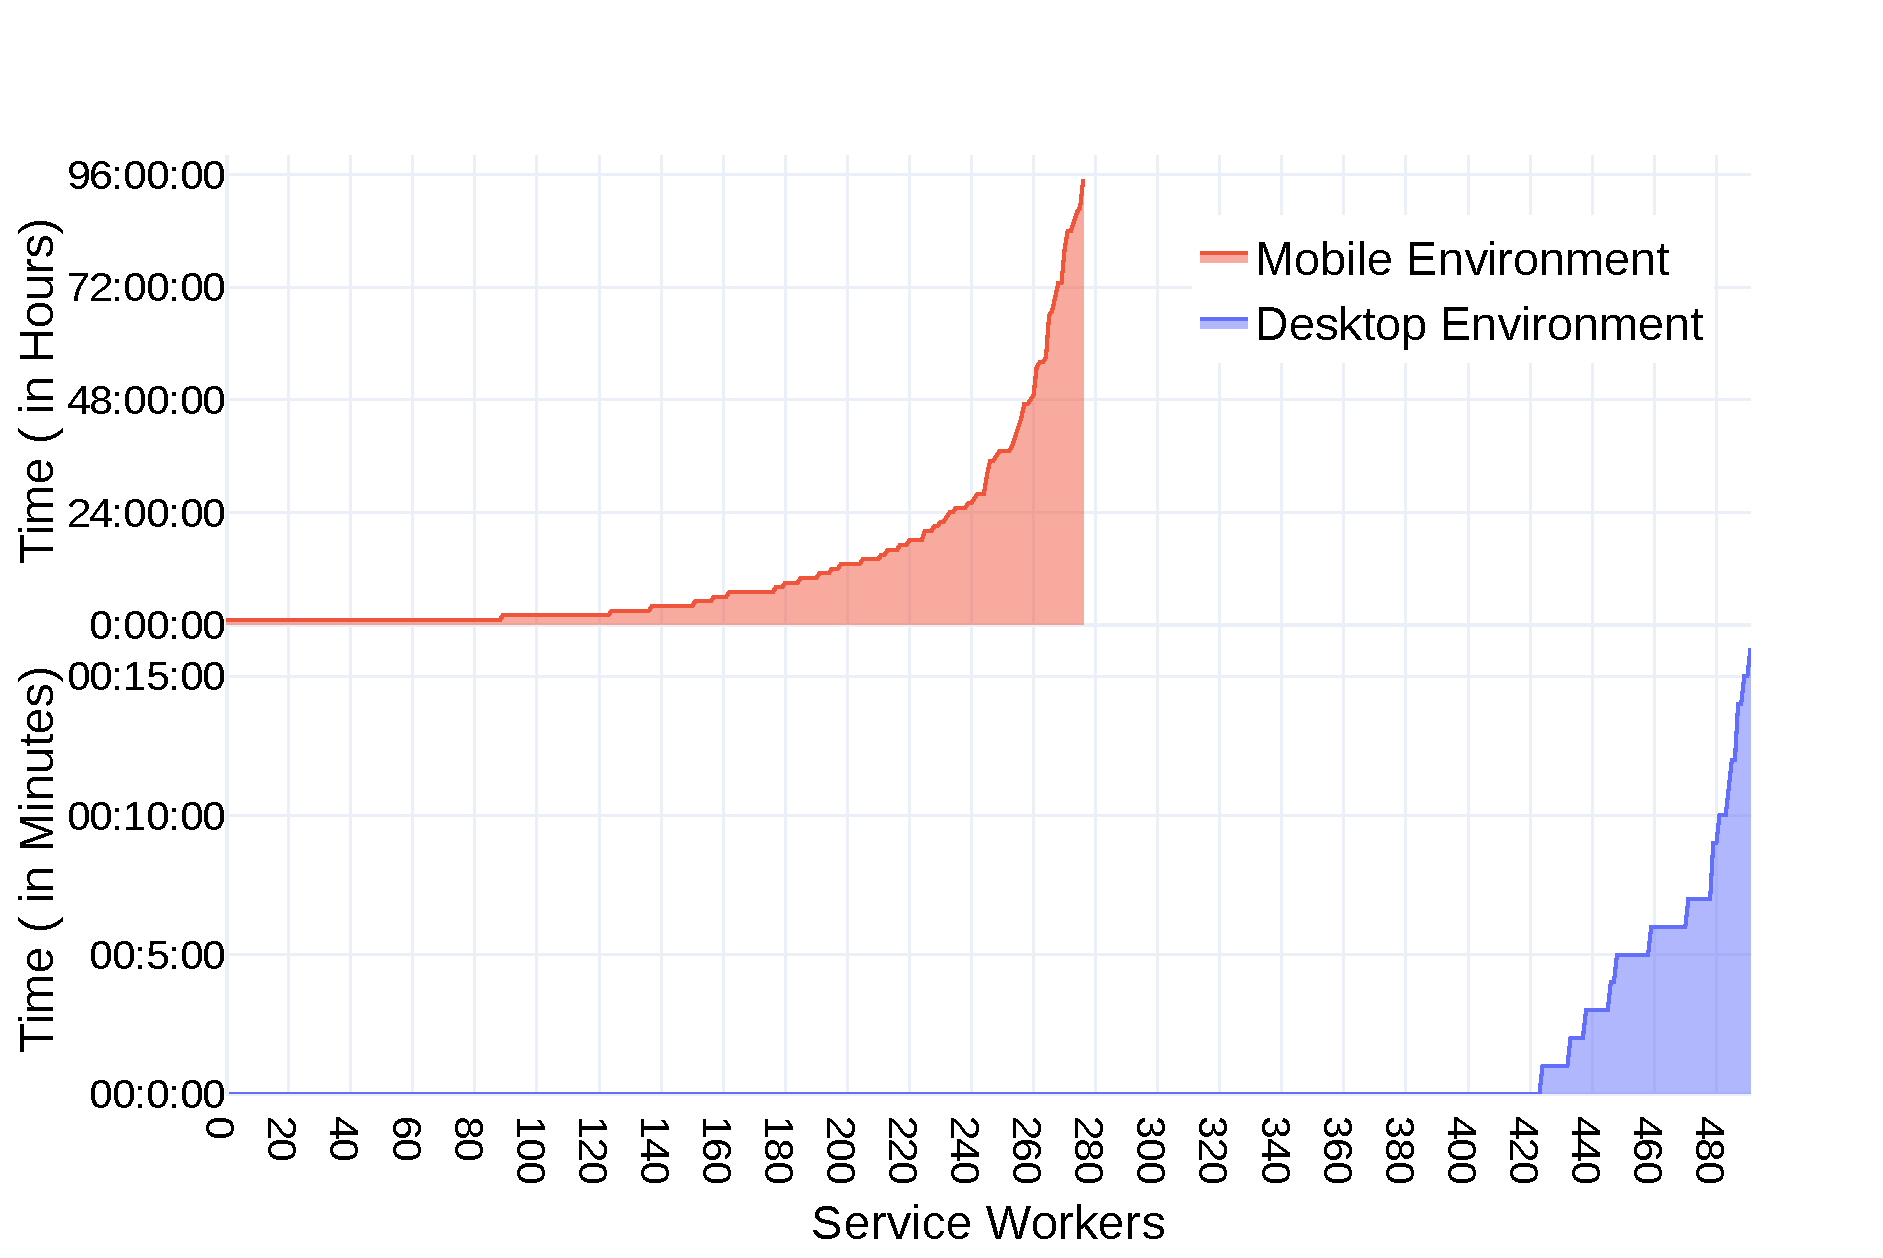
\includegraphics[width=\columnwidth]{figs/first_notifications.pdf}
% \caption{Time taken for websites to send their first notification}
% \label{first_notification}
% \end{figure}


% \begin{figure}[h]
% 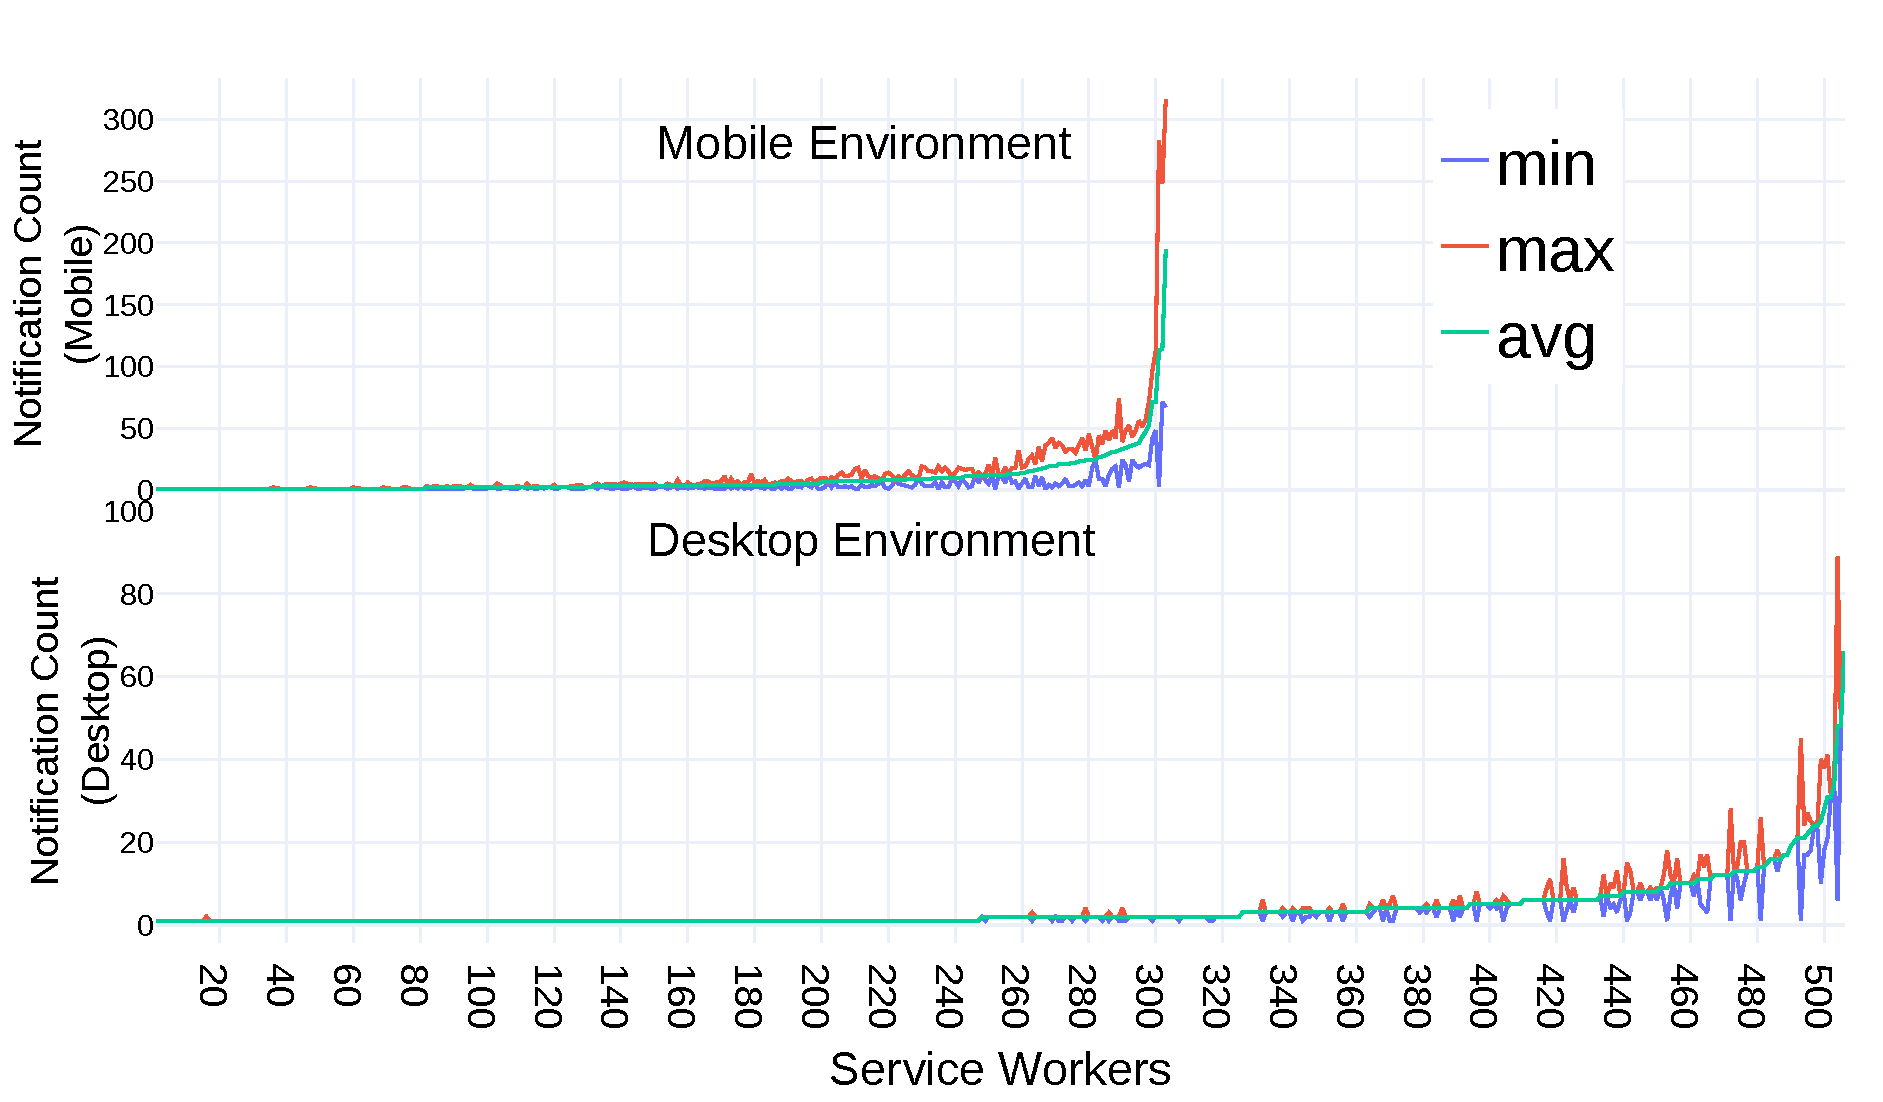
\includegraphics[width=\columnwidth]{figs/avg_not_dm.pdf}
% \caption{Number of notifications per day}
% \label{notification_per_day}
% \end{figure}

\begin{figure}[h]
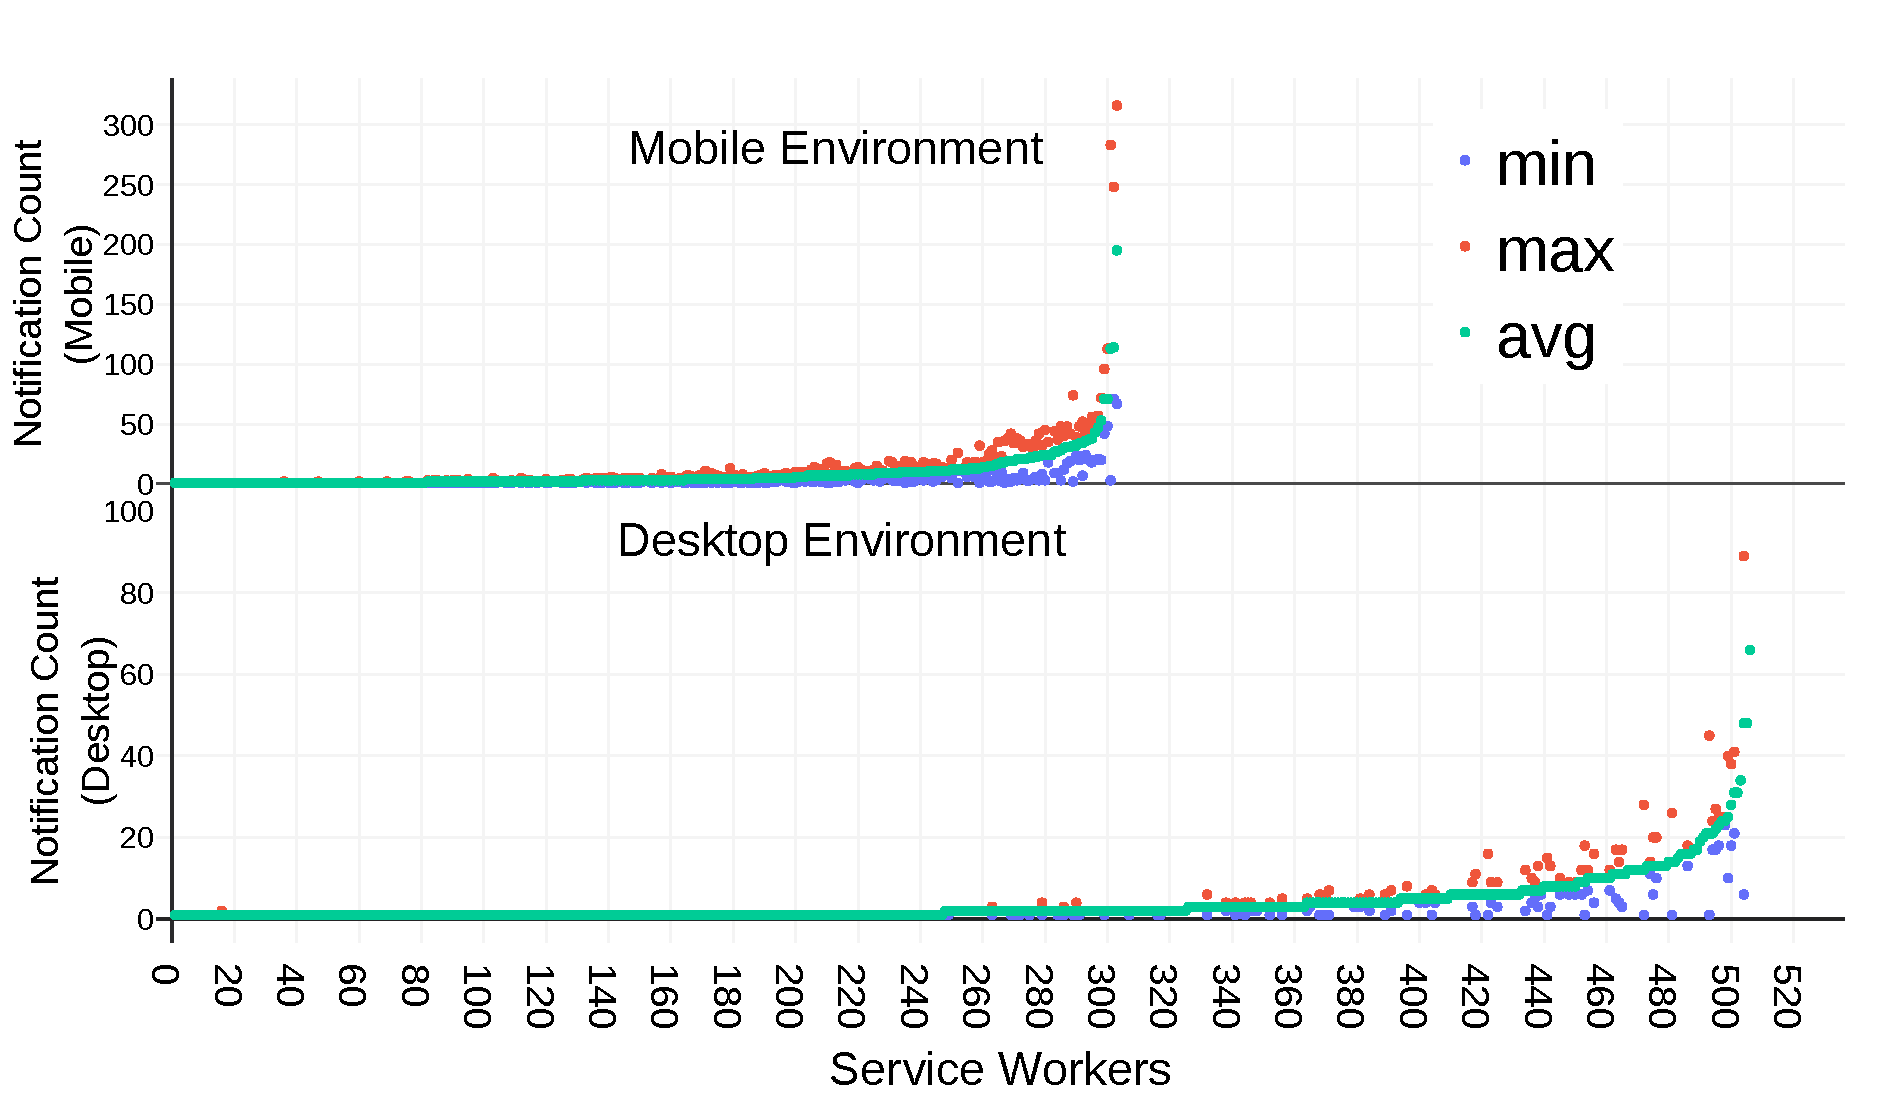
\includegraphics[width=\columnwidth]{figs/avg_notifications.pdf}
\caption{Number of notifications per day}
\label{notification_per_day}
\end{figure}

\subsection{Advertisements, their properties and patterns}
In this section, we explain in detail how we identify various ad campaigns, ad networks responsible for the campaigns and determine the maliciousness of the ads. At the end of our data collection stage, we had logged over 5000 and 3000 notifications in desktop and mobile environment. Over 20\% of notifications collected belong to languages other than English. We make use of Google Translate's online service to translate as many notifications as possible to English. The different information we found useful for the next stages of analysis are notification title, notification body, service worker file , landing URL, website's trust score, landing domain's trust score, IP address and WHOIS information of landing domain and the first domain contacted by the service worker and the data from Google safe browsing list and Virus total blacklists. Due to large amount of data and it's information, we perform a layered clustering of data. At each layer of clustering, we consider different sets of information that would identify the patterns if any among the ads and ad networks. The multiple layers are explained in the following sections

\subsubsection{Discovering Ad Campaigns}
Ad campaigns are defined as set of advertisements that delivers a similar message and are created with a particular goal. From a security perspective, we consider ad campaigns to be the set of ads that follow similar pattern with their main goal as 'to attract as many user clicks' as possible. To obtain advertisements with similar message/pattern, we consider the features notification title and notification body. We use the combined text of both features and clean them for stop words, convert any smileys into their word representations using \ref{simley_to_text} and vectorize the data. We use \texttt{gensim.similarities.SoftCosineSimilarity} to calculate the similarity between the samples. We chose soft cosine similarity measure over Jaccard and Cosine similarity measure as the former is known to identify the slightest common patterns between two given sentences compared to the latter ones \ref{soft_cosine}. Then, we perform an Agglomerative Hierarchical clustering on the distance matrix calculated from the soft cosine similarity matrix. We performed agglomerative clustering for various clusters based on the dendogram as shown in fig \ref{dendogram}. We then manually analyzed the results for few cut-offs to determine the best cut-off as 0.7 for which the clusters had relevant samples.Some examples of these clusters are shown in Fig.\ref{text_cluster}.  At this cut-off, the algorithm clustered 2700 samples into 750 clusters. 

%% change explanation using silhoutte score for the clusters

\begin{figure}[ht]
\caption{Examples of Ad Campaigns }
\begin{center}
\label{text_cluster}
\begin{tabular}{c}
\hline


 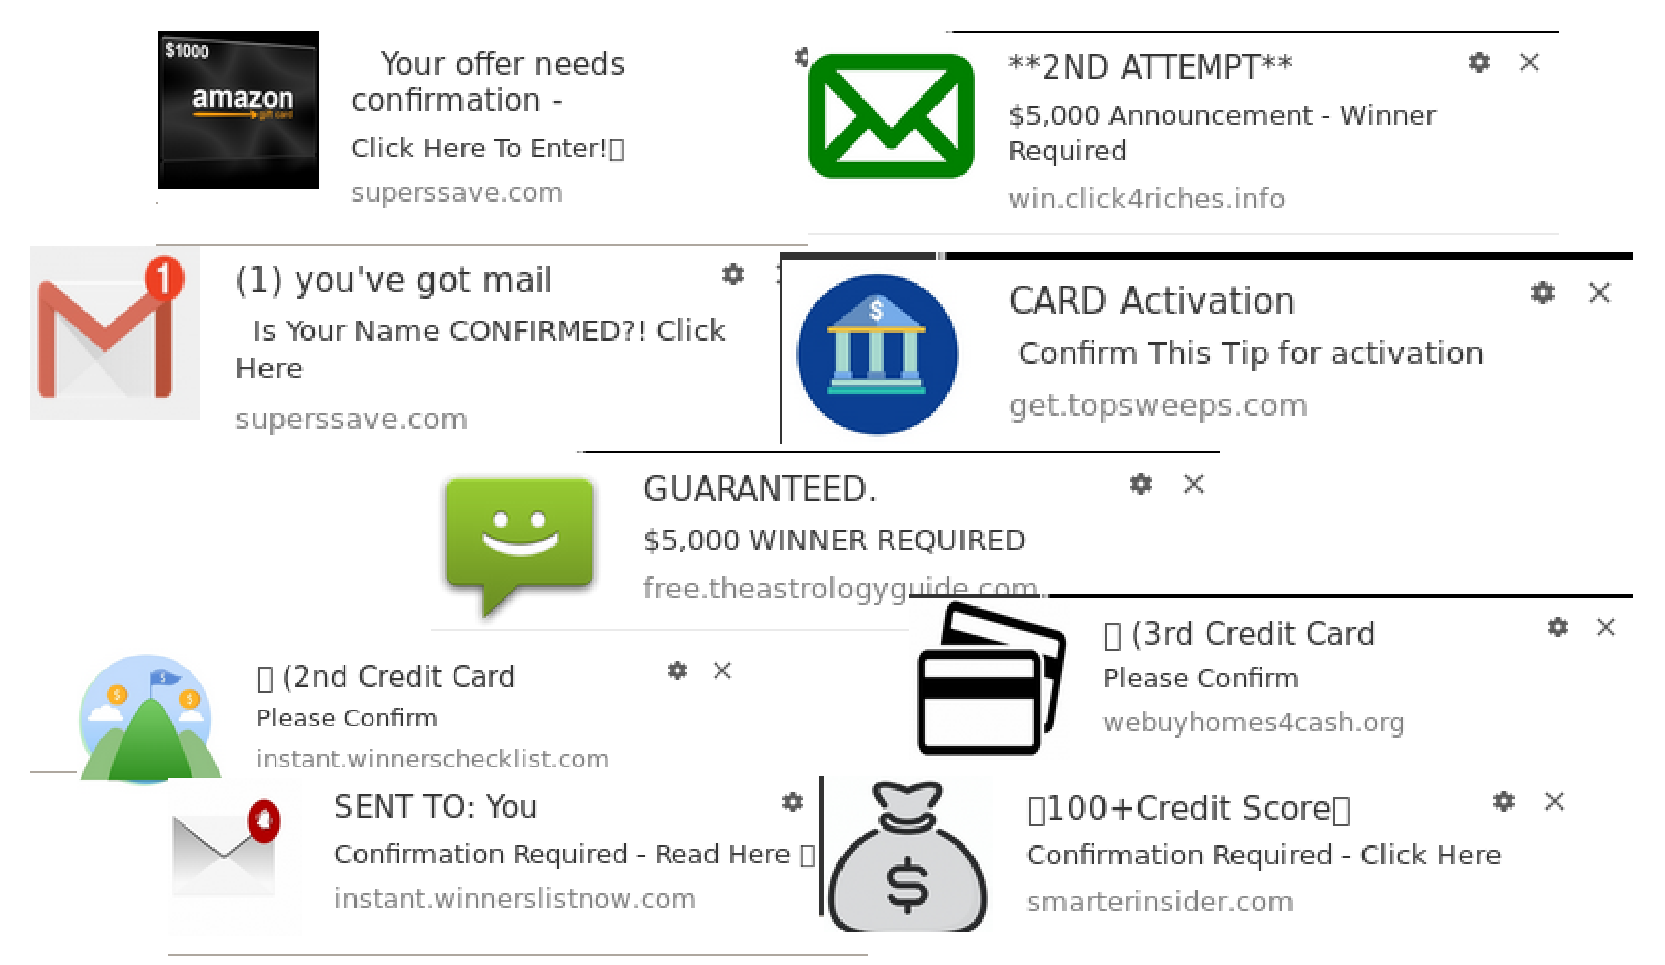
\includegraphics[scale=0.28]{figs/notifications.pdf}{C1}

\\
\hline
\hline

 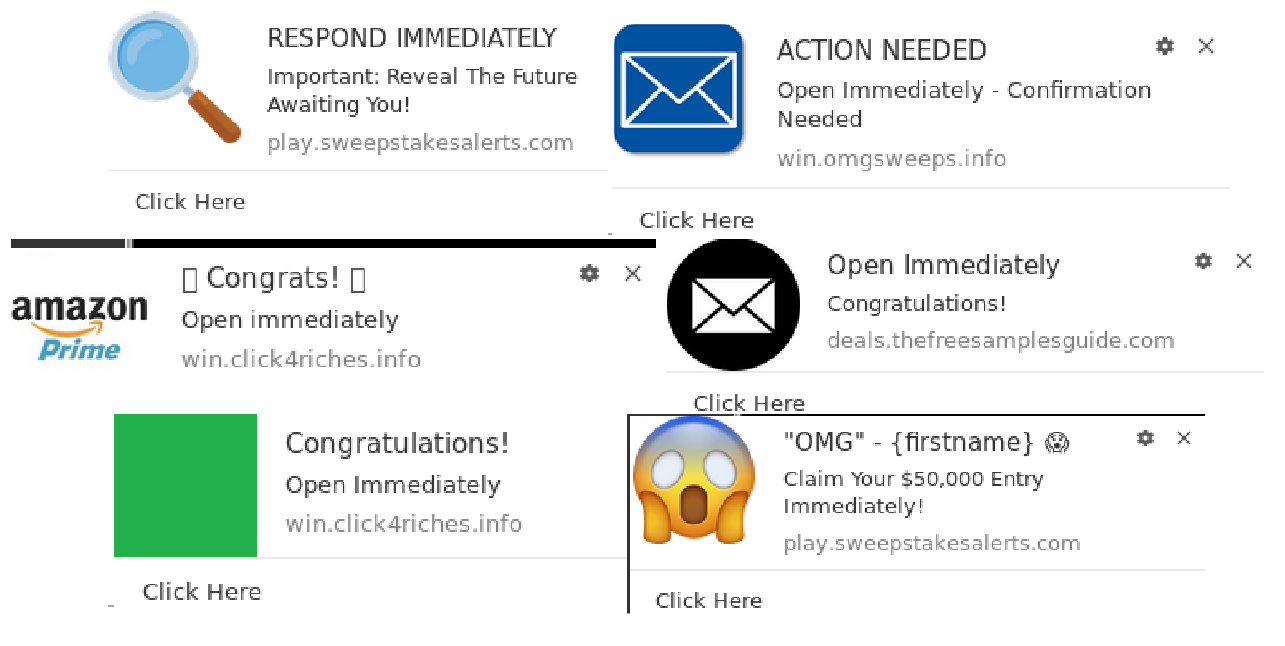
\includegraphics[scale=0.28]{figs/notifications2.pdf}{C2}

 \\
 \hline
    \end{tabular}
\label{tab1}
\end{center}
\end{figure}


\subsubsection{Topic Detection on Clustered Advertisements}
Looking over the clusters manually, we found a lot contextual similarity between the ads that belonged to a cluster and across clusters. To obtain a higher sense of the topics each clusters dealt with, we performed a topic modelling on the clusters using LIWC dictionary \ref{LIWC}. AS each advertisement has fewer number of words, we merge the samples that belong to each clusters and provide it as input to the topic modeller. From the topics listed by LIWC dictionary, we removed the topics related to linguistics and was left with 32 topics. The Fig. \ref{topic_cloud} illustrates the distribution of these topics among the ad clusters. We use these topics discovered for each ad cluster in next stage of clustering. The word cloud tells us that most of the advertisements we gathered had tried to attract users by trying to reward them with money or gifts. On the contrary, we also found a number of notifications focused on scaring the users into clicking ads regarding their bank accounts, health issues and mails.

\begin{figure}[ht]
\begin{center}
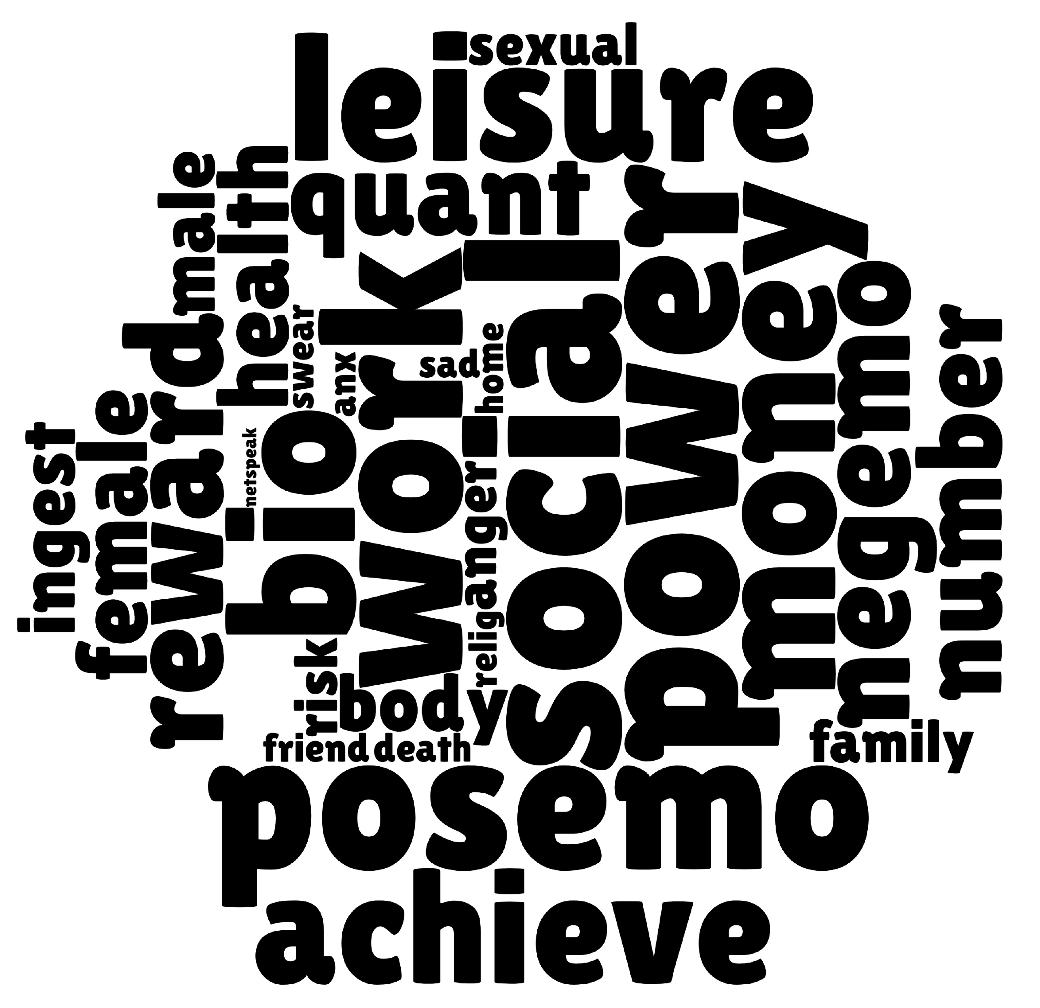
\includegraphics[ scale=0.4]{figs/topic_cloud.pdf}
\caption{Word Cloud on Topics detected in collected ads }
\label{topic_cloud}
\end{center}
\end{figure}


\subsubsection{Discovering Similar Behaviour in Advertisements and Ad Networks}
This is the third and final layer of clustering. At this stage, we use the features mentioned in table \ref{features} to cluster the advertisements. This clustering brings together advertisements that lead to same URL or IP address or location; belong to same ad network; deal with similar topics. To achieve this, we used K-means clustering with 3000 advertisements as input and obtained 250 clusters.

\begin{table}[htbp]
\caption{Features }
\begin{center}
\label{features}
\begin{tabular}{p{2.5cm}|p{5.5cm}}
\toprule
\hline
 \textbf{Features} & \textbf{Explanation}
 \\
 \hline
 Ad Campaign Ids & Output from First stage of clustering on notification title and body 
 \\
  \hline
 Ad Topics & Topics obtained from detection  using LIWC dictionary
 \\
 \hline
 Ad Network Domain & First Domain that the service worker contacted after registration
 \\
  \hline
 IP address & IP address of the final URL the advertisement leads user to 
 \\
 \hline
 Landing Domain & Domain name of the final URL the advertisement leads user to 
 \\
 \hline
 Latitude & Latitude of the landing URL's IP
\\
\hline
 Longitude & Longitude of the landing URL's IP
\\
 \hline
 WHOIS name & Party responsible for registering the landing domain
 \\
 \hline
 \bottomrule
\end{tabular}
\end{center}
\end{table}

\noindent \textbf{Categorizing Push Advertisements}
During the analysis of clusters, we categorize advertisements based on the content of their landing page. Different categories that we came across in our samples and the number of URLS for each cases are shown in \ref{categories}. Since visiting each page to determine it's category involves a lot of manual effort, we only visit a subset of our data samples. For example, We don't try and visit those cases that are in languages other than English as we might not fully understand it's content and hence fail in categorizing them. On analyzing these chosen samples, we found certain ads and the landing pages to be suspicious. We consider suspicious advertisements to be the ads that lead user to known malicious pages or to pages that appear to be phishing or scam pages built to deceive users or to pages that are irrelevant to the advertisement's context. We use multiple parameters to determine if an advertisement is suspicious in nature. 

\begin{itemize}
    \item To identify known malicious domains and pages, we check the URLs that we come across during our experiments on Google Safe Browsing(GSB) and Virus Total reporting tool.
    \item Next, We submit the URLs on Virus Total's scanning platform. This platform scans the submitted URLs in the background and update the results about their maliciousness. This identifies malicious pages that are not blacklisted until we submitted them as suspicious URLs.
    \item If a sample in a cluster is found to be malicious, we suspect other members of the cluster and perform detailed analysis on those samples
    \item We consider same ads leading to multiple landing pages within a single cluster as suspicious.
    \item If there are multiple landing domains/ URLs following the same naming/URL pattern, we tag them suspicious for further manual verification.
\end{itemize}
   
To our surprise, we found that the most popular blacklists available such as GSB and Virus Total were unaware of lot of URLs that we scanned with them. When we submit the URLs to GSB, we do not reveal the URL but send a hash of the URL to GSB. This method lets us measure the time taken for GSB to blacklist a URL that is malicious since we first encounter it. To reduce the manual effort on deciding if a page is malicious, we then submit the URL for scanning on virus total and check the report later to obtain the result. We check the reports for all the URLs at regular periods of time in both GSB and Virus Total. The results from these two tools showed a total of X number of URLS/domains to be malicious with GSB listing Y and Virus Total listing Z as malicious. However, on manual analysis we found a number larger than the total number reported by the tools. We were able to identify over XX number of URLs as malicious. 

\section{Case Studies}
In this section, we explain with the help of case studies the effectiveness of our clustering method to identify relevant samples and discuss few malicious cases that we encountered during our analysis and the relation between them.

\subsection{Phishing Via WPN Ads}
This case study discusses how Web Push Notification(WPN) service is being used by some adversaries to deliver spoofed pages to the end users. In traditional phishing method, the success rate of an adversary in delivering phish links to the users is quite low as they have to overcome multiple defenses to reach the end user. However, advertisements that are sent using WPN are delivered directly to the user without any additional filtering/monitoring done by Ad blockers. Few cases that we encountered from one of the result clusters contained advertisements that led to spoofed pages of popular news websites such as CNN, Fox News and Entertainment Today. This phenomenon could be observed from Fig.\ref{fake_news}. To be specific, the domains of these landing pages are \texttt{appearsnews.com(bottonm-left),  producednews.com(top-left), usa-health-news.com(center \& bottom-right)} and \texttt{ healthydreamstoday.com(top-right)}. It has to be noted that the domain \texttt{usa-health-news.com} serves spoofed pages of two different news sites. Further analysis of these cases revealed that none of them share an IP address. However, on analyzing the ownership details of the domains, we found that the domains \textbf{appearsnews.com \& producednews.com} and domains \textbf{usa-health-news.com \& healthydreamstoday.com} belong to the same domain registrant. A look up of these landing URLs on GSB and Virus Total gave us no results. While scanning the URLs on Virus Total, we found that these URLs were not known to it until we submitted them for a scan. this implies that phishing pages served through WPNs stay alive for a longer time period compared to traditional pages that are usually short-lived before they get noticed by one of the known blacklisting tools. 

\begin{figure}
\begin{center}
 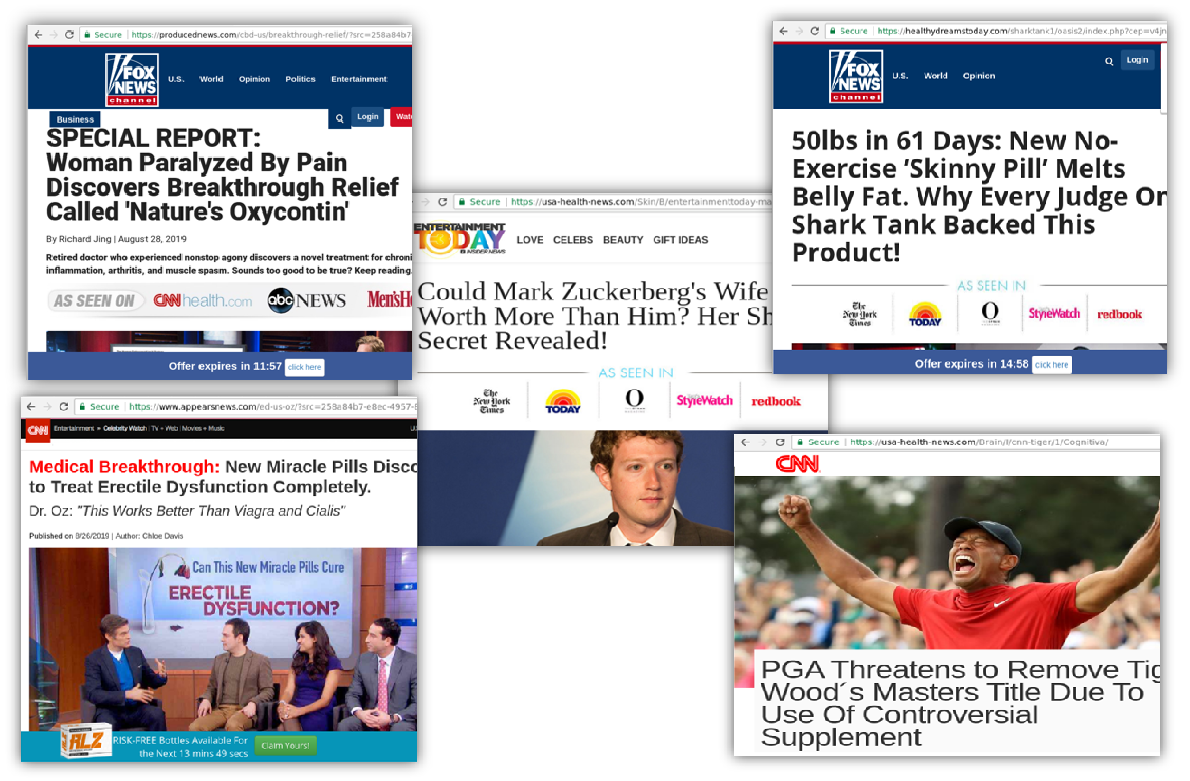
\includegraphics[width=\linewidth]{figs/fake_news.pdf}
        \caption{Example of Phishing on Popular News sites obtained via WPN Ads}
        \label{fake_news}
\end{center}
\end{figure}


\subsection{McAfee Ad Campaign}
This case study is about one of the ad campaigns that we encountered. In this Ad campaign, websites sent ads to the users mentioning that their McAfee antivirus software's license has expired and that they need to renew their McAfee subscription. From our clustering results, we had over 100 advertisements belonging to McAfee ad campaign clustered into a single cluster. This cluster had ads leading users to multiple landing domains. On observing the cluster keenly, we found a few different domains that belong to the same ip address. The cases observed were obtained when \sysname had visited \texttt{https://mogye.info} and \texttt{https://hotmovs.info}. By default, \sysname grants permission to both domains to send notifications. These ads shown by these domains to the user regarding McAfee ad campaign are shown in Fig.\ref{McAfee_case}. After \sysname had clicked these advertisements, these ads had led to domains \texttt{exclusivebreakingstory.com, business-giveaways.com, newtrendingstory.com} and \texttt{hottrendingstory.com}. Moreover, three of these domains resoles to the same IP address '104.238.196.100' and these domains seem to follow a similar pattern. Therefore, we did a reverse-IP lookup on the IP address and found more domains from the same IP address that follow the same pattern. Later, we found that same registrant had registered the discussed 11 domains from the IP address '104.238.191.100'. It has to be noted that none of these landing URLs were accessible later outside it's session. It is interesting to note that domains such as \texttt{healinggreencoffee.com} and \texttt{solutionquotes.com} are involved in this campaign. On trying to find more information on these domains, we found a google result attributing the domain \texttt{healinggreencoffee.com} (refer Fig.\ref{google_res} to a medical news wen page which is another ad campaign that we have observed in our results. Similar to other pages, this page was inaccessible for further enquiry.This search also led us to a report of IP '104.238.196.100' on \texttt{https:/abuseipdb.com} (refer Fig.\ref{ip_report}) which mentioned that the IP was reported over 7 times for phishing, spam and fraud orders. 

\begin{figure}[ht]
\begin{center}
 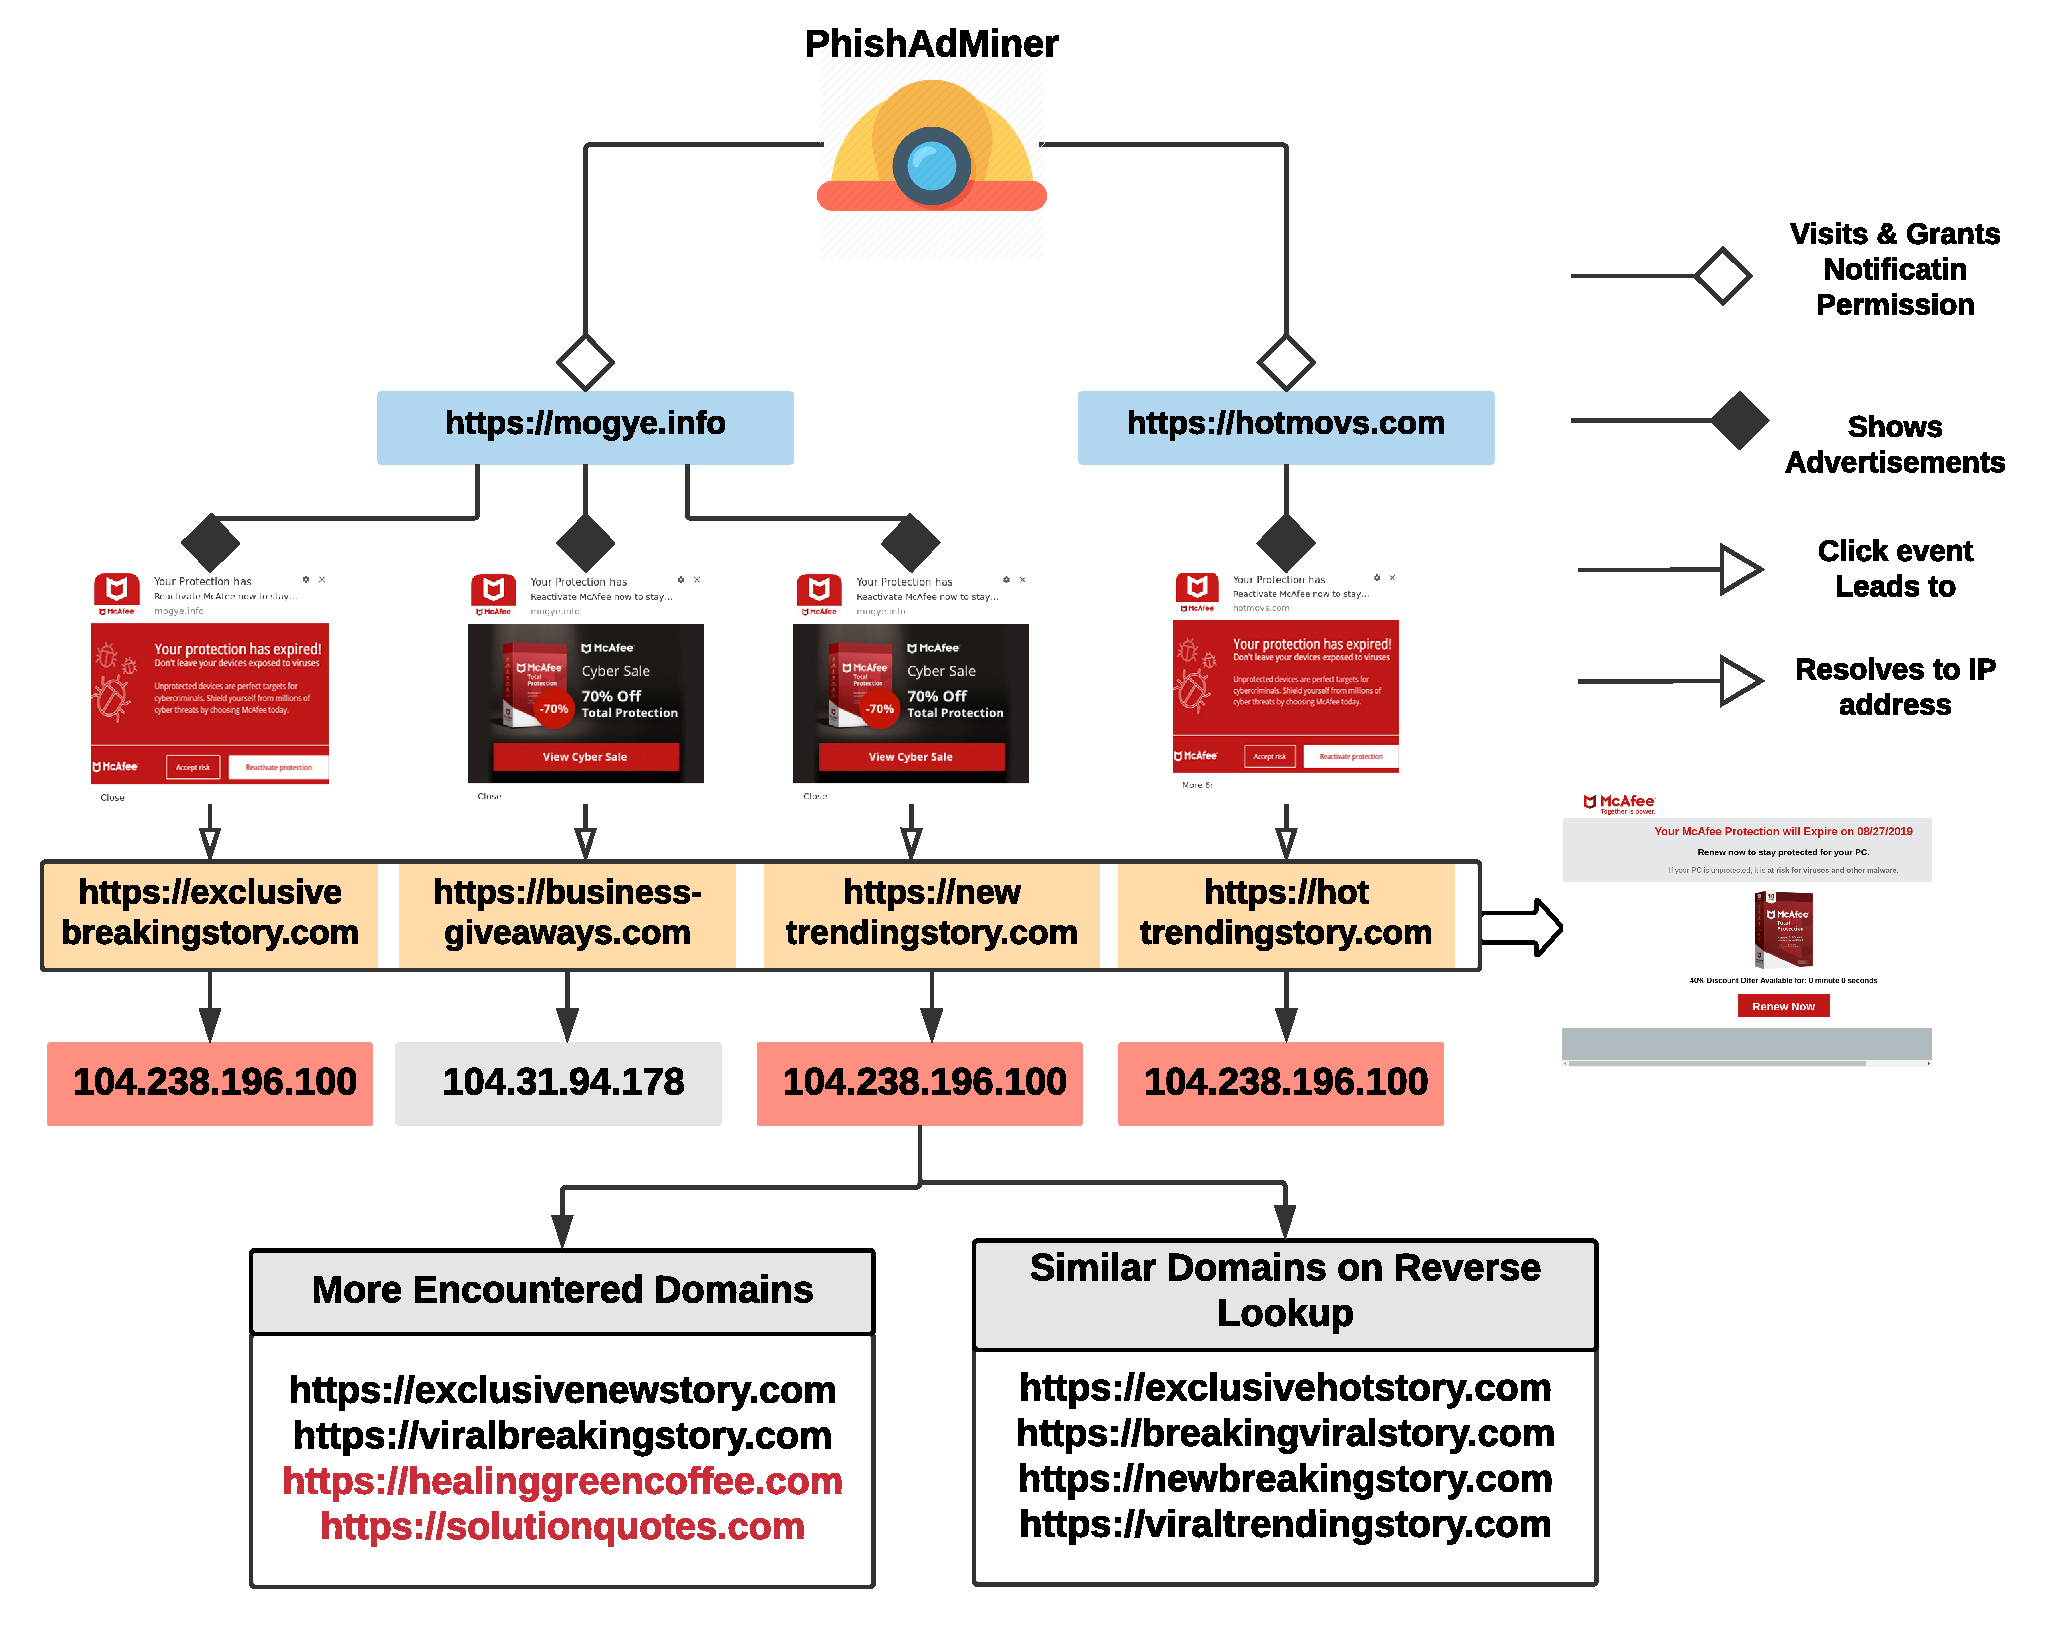
\includegraphics[width=\linewidth]{figs/mcafee_case2.pdf}
        \caption{Case study on McAfee Ad Campaign}
        \label{McAfee_case}
\end{center}
\begin{center}
 
\includegraphics[width=\linewidth]{figs/healinggreencoffee.png}
        \caption{Searh Result on the domain 'healinggreencoffee.com'}
        \label{google_res}
\end{center}
\begin{center}
 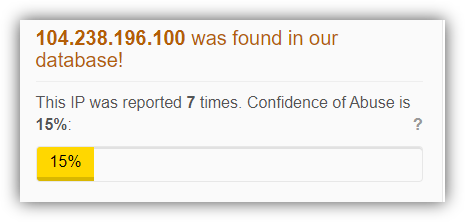
\includegraphics[width=\linewidth]{figs/ip_report.png}
        \caption{Report on the IP '104.238.196.100'}
        \label{ip_report}
\end{center}
\end{figure}

Considering this case is suspicious enough, we follow to check on the other domain that belongs to this cluster \texttt{business-giveaways.com}. Although, we couldn't decide on it's maliciousness by visiting the landing page, on obtaining the registrant information from WHOIS domain, we found that this domain belongs to the same individuals who had registered the domains \texttt{usa-health-news.com, appearsnews.com, healthydreamstoday.com} that were discussed in the previous case study. Based on the fact that, the domians from previous case study served fake news via phishing and the current domain 'business-giveaways.com' as well is registered from the same individual, we tag 'business-giveaways.com' as suspicious/malicious domain. Therefore, our clustering proved to be an efficient way to identify similar ad campaigns and discover similar cases effectively.


%%%%%%%%%%%%%%%%%%%%%%%%
\subsection{Mobile targeted click-bait}
In this section, we discuss cases that were tailored to specifically target mobile users into clicking the notification. In Mobile environment, we encountered a lot of ads that are fake 'Missed Call' messages. Few of such advertisements are shown in Fig. \ref{fig:mobile_disguised_notification}. Note that in Fig. \ref{fig:mobile_disguised_notification}(b), the third notification is a fake Amber Alert with the city name of the test device we have. Because website server can get visitor's IP address, it is fairly easy to the obtain the geographic location of that IP address. By doing so, the fake notification would appear more legitimately to the users. Further, we analyzed one of the cases manually to figure out the motive behind such advertisements. The case that we analyzed in detail is portrayed in Fig. \ref{fig:mobile}. In this example, the ad shows '1 Missed Call' message. When an user clicks on it, it first lands in a web page saying "You will lose 14kg in 28 days.". Then after a few seconds, it automatically redirects to a page selling the drug. To urge the users into buying the drug before the offer expires or before the drug is unavailable, the page displays a countdown for 3 minutes. Once the user agrees to buy the drug, the website composes several forms, aiming at collecting sensitive information like phone number, email address and contact address. As it can be observed from Fig. \ref{fig:mobile_disguised_notification}(a), when there appear a large number of notifications, information regarding the sender application and domain name are hidden to make space for new notifications\samuel{I'm not quite sure what this means. I can still see "chromium" and domain names in the notification. If the user wants to click the notification below, he needs to scroll up and expand those notifications. At that time, the app name and domain name will be shown.}. This proves to be significant way for scammers to trick mobile users and can lead to potential loss of significant information for the users.

% The case in Fig. \ref{fig:mobile} is an example of mobile specific click-bait. The notification will be disguised as other application's notification and lure users to click, in this case, it first lands in a web page saying "You will lose 14kg in 28 days.". Then after a few seconds, it redirects itself to a page selling the drug. To make users feel urgent and purchase the drug fast without thinking it through, it even puts a 3 minutes countdown. Then after this point, the website composes several forms, aiming at collecting sensitive information like phone number and email address. There are more examples shown in Fig. \ref{fig:mobile_disguised_notification}. Noted that in Fig. \ref{fig:location}, the third notification is a fake Amber Alert with the city name of out test device. Because website server can get visitor' IP address, it is fairly easy to the obtain the geographic location of that IP address. By doing so, the fake notification would be more appealing.


\begin{figure}[h]
\begin{center}
    \begin{subfigure}{.2\textwidth} 
    \begin{center}
        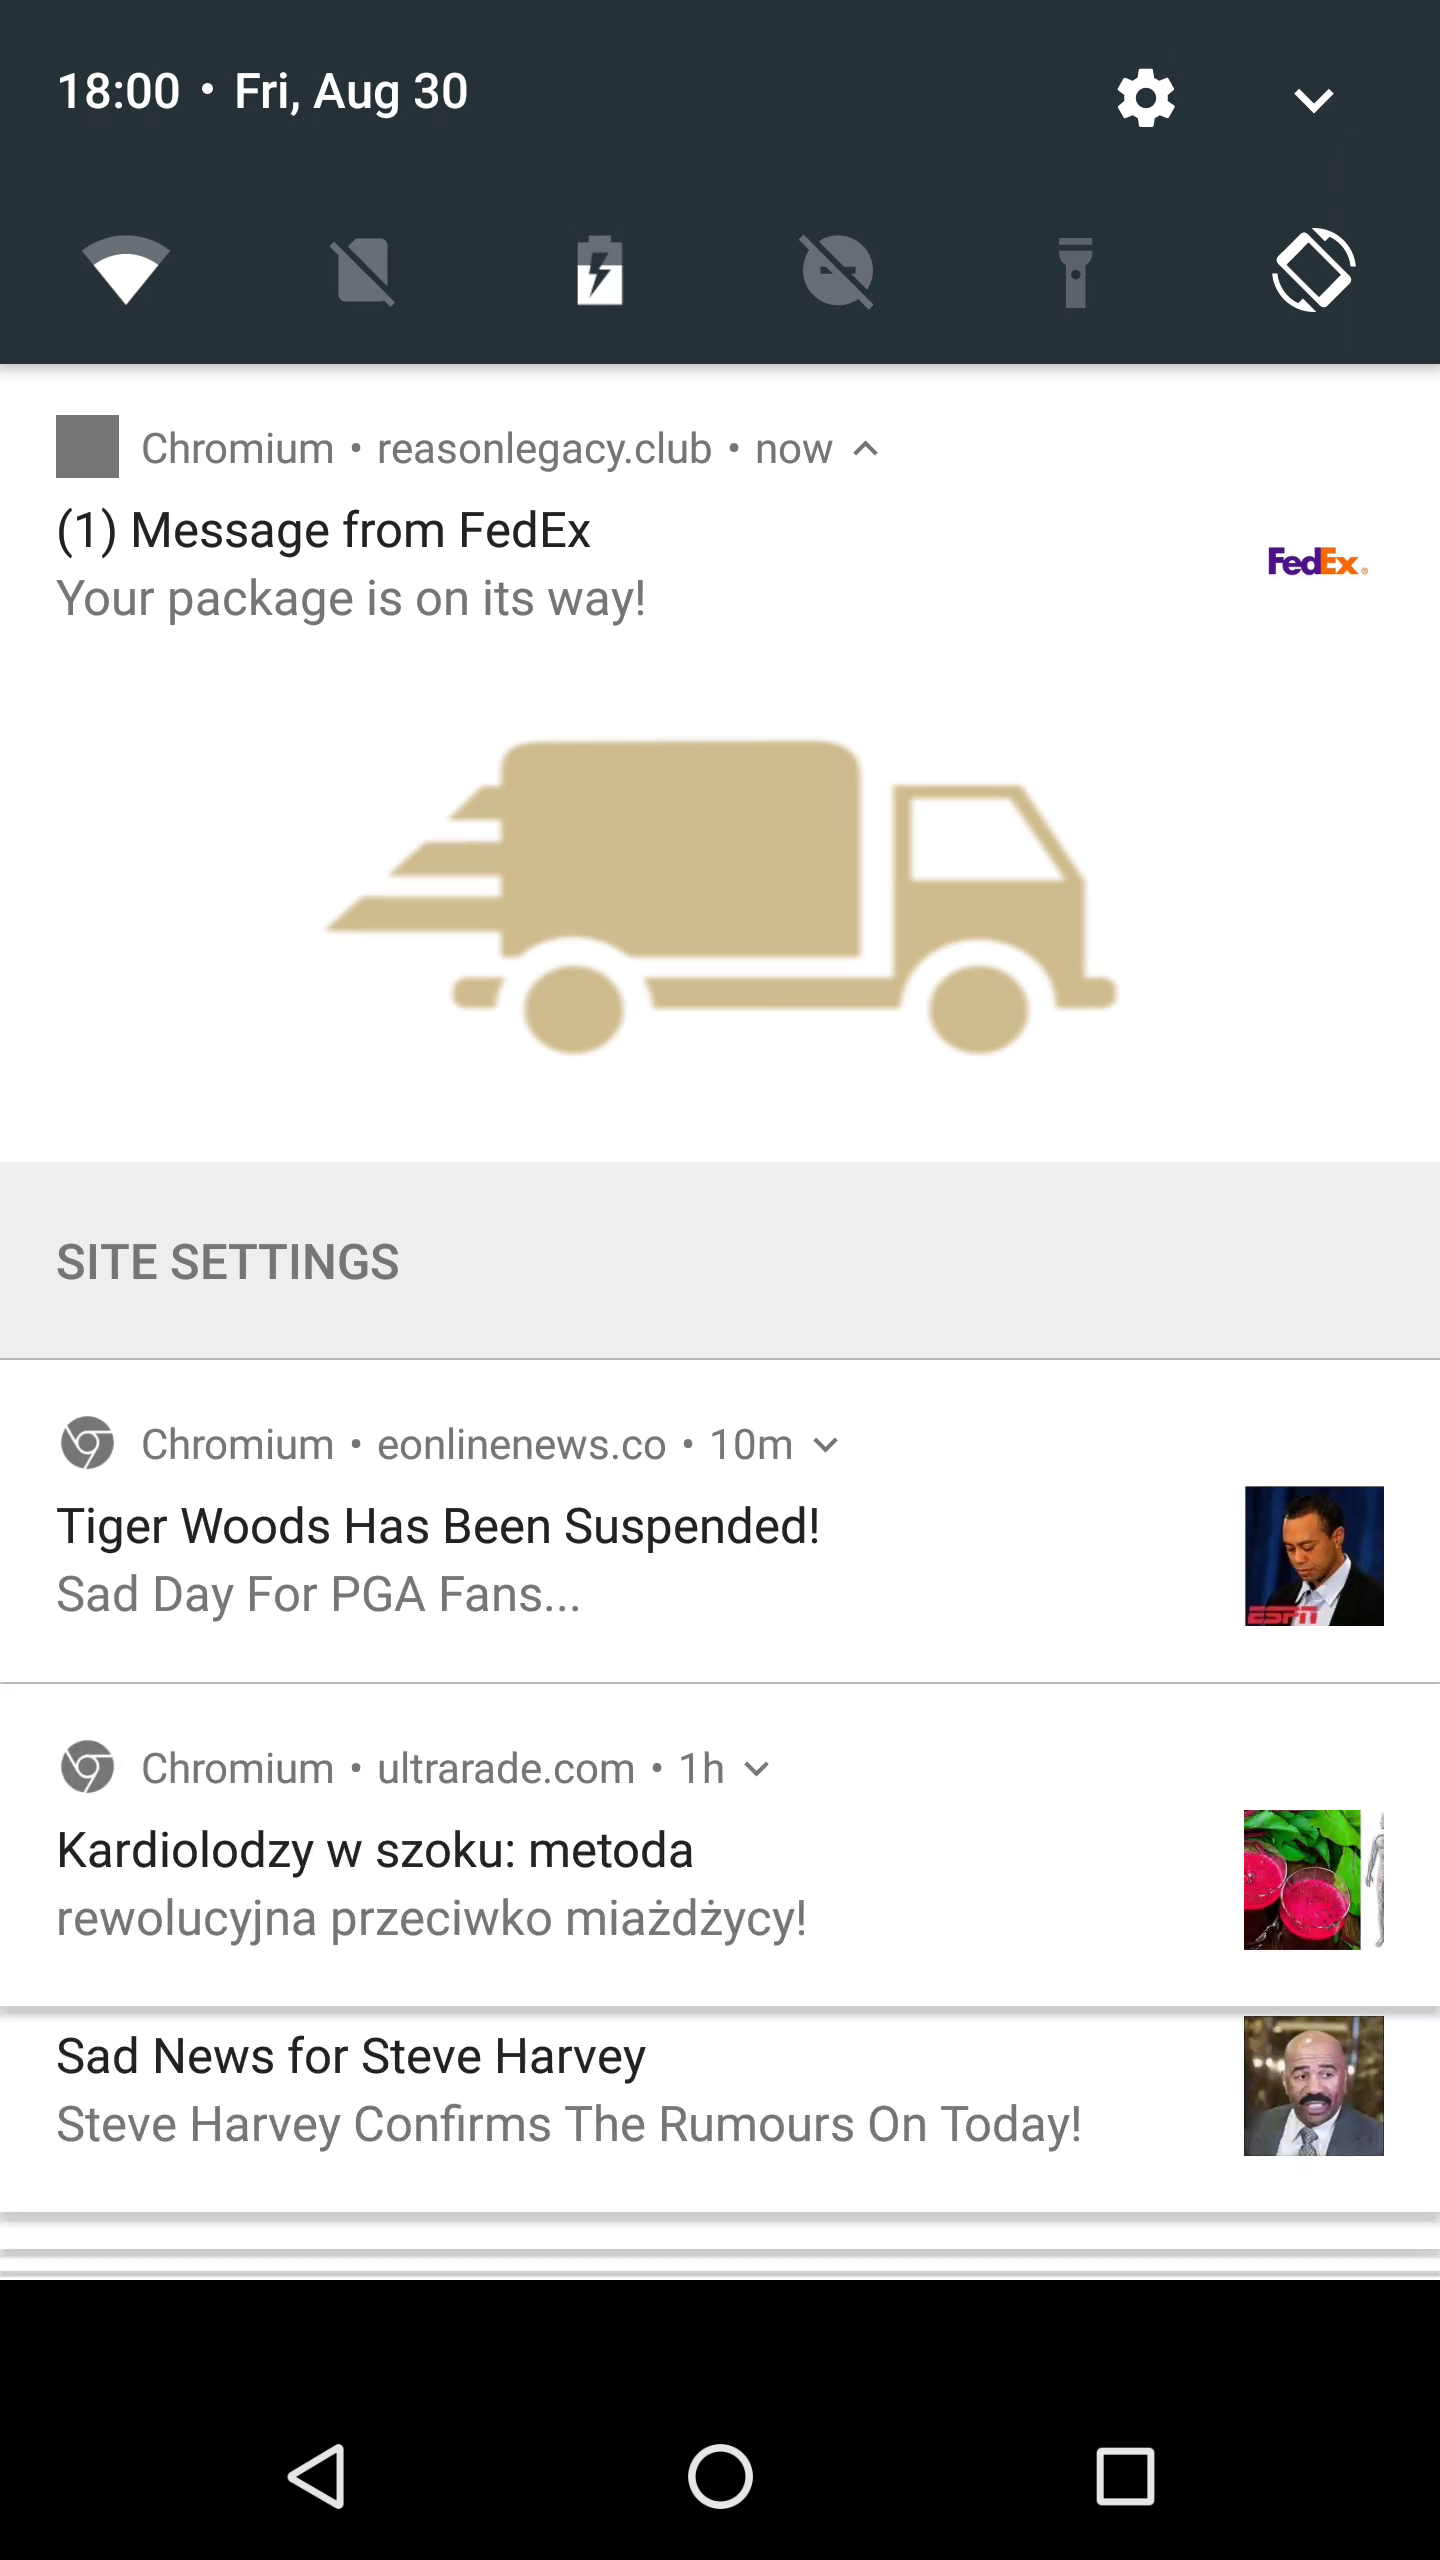
\includegraphics[width=\linewidth]{figs/mobile_disguised_2}
        \caption{}
    \end{center}
    \end{subfigure}
    \begin{subfigure}{.2\textwidth} 
    \begin{center}
        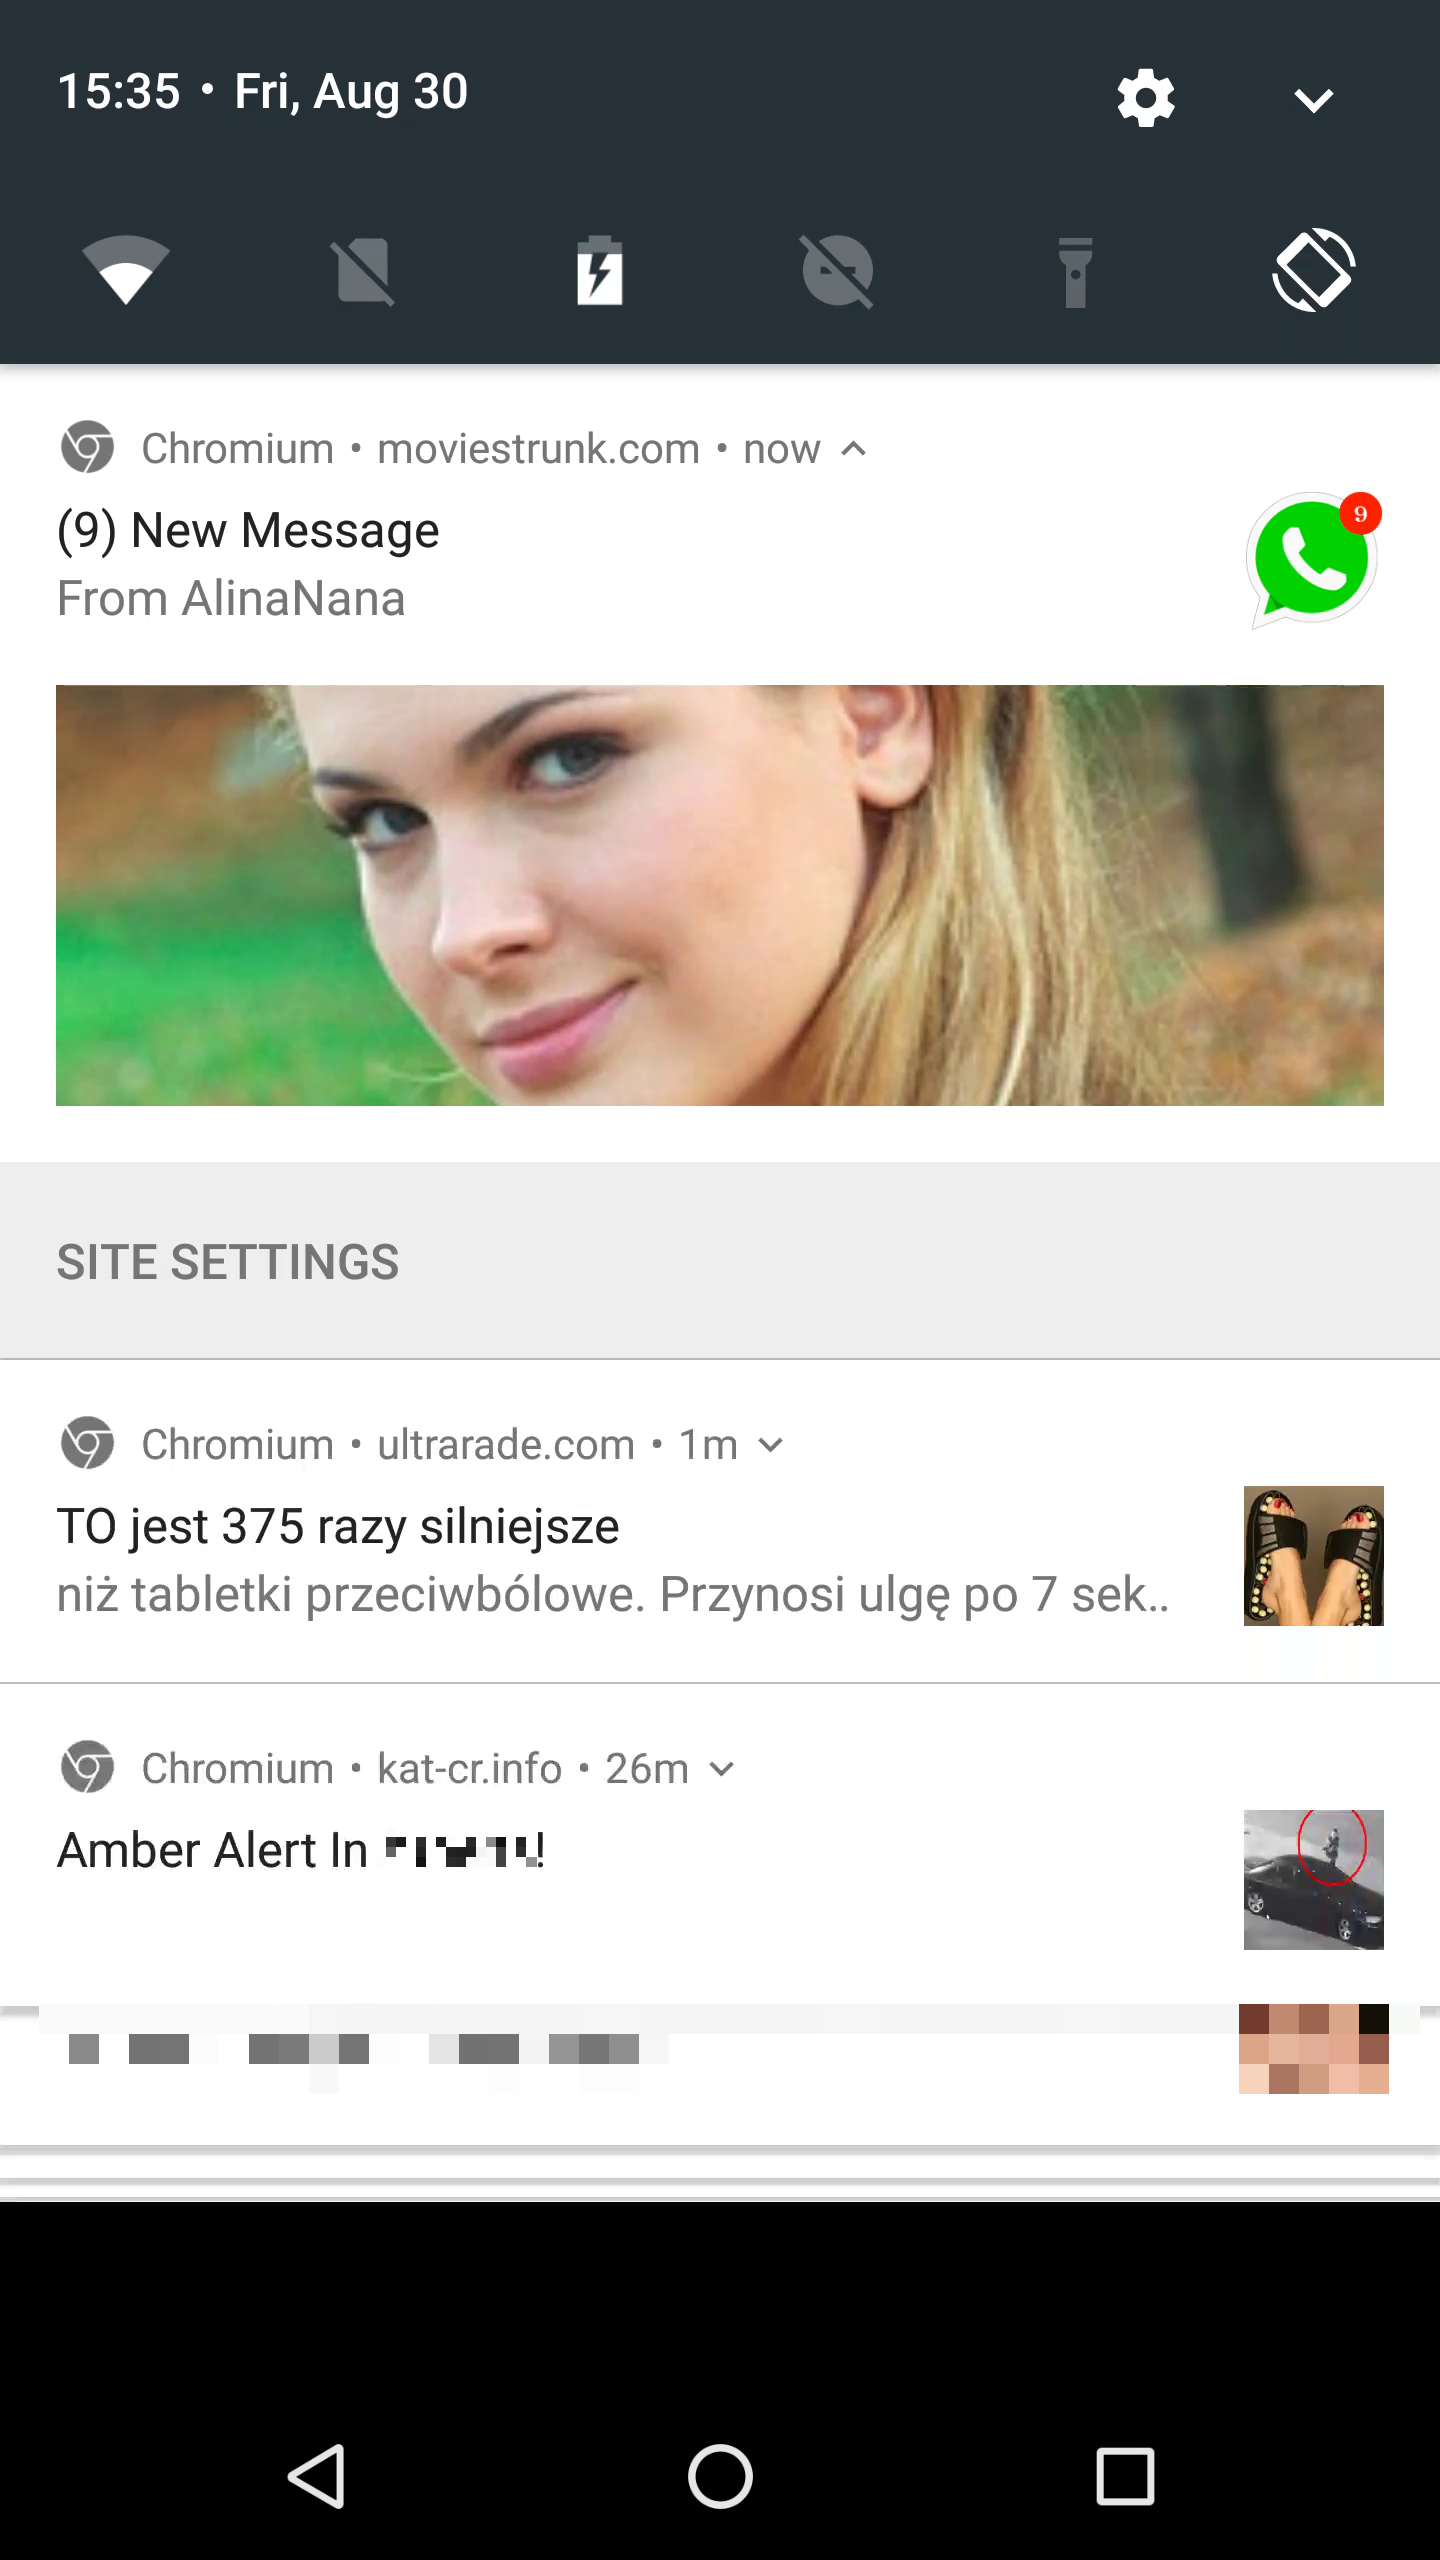
\includegraphics[width=\linewidth]{figs/mobile_disguised_3}
        \caption{}
        \label{fig:location}
    \end{center}
    \end{subfigure}
    \caption{Click-Bait Examples on Mobile: (a)Ad disguised as Fedex app's notification (b)Ad disguised as WhatsApp's notification}
    \label{fig:mobile_disguised_notification}
\end{center}
\end{figure}


\begin{figure*}[h]
\begin{center}
    \begin{subfigure}{.18\textwidth}
    \begin{center}
        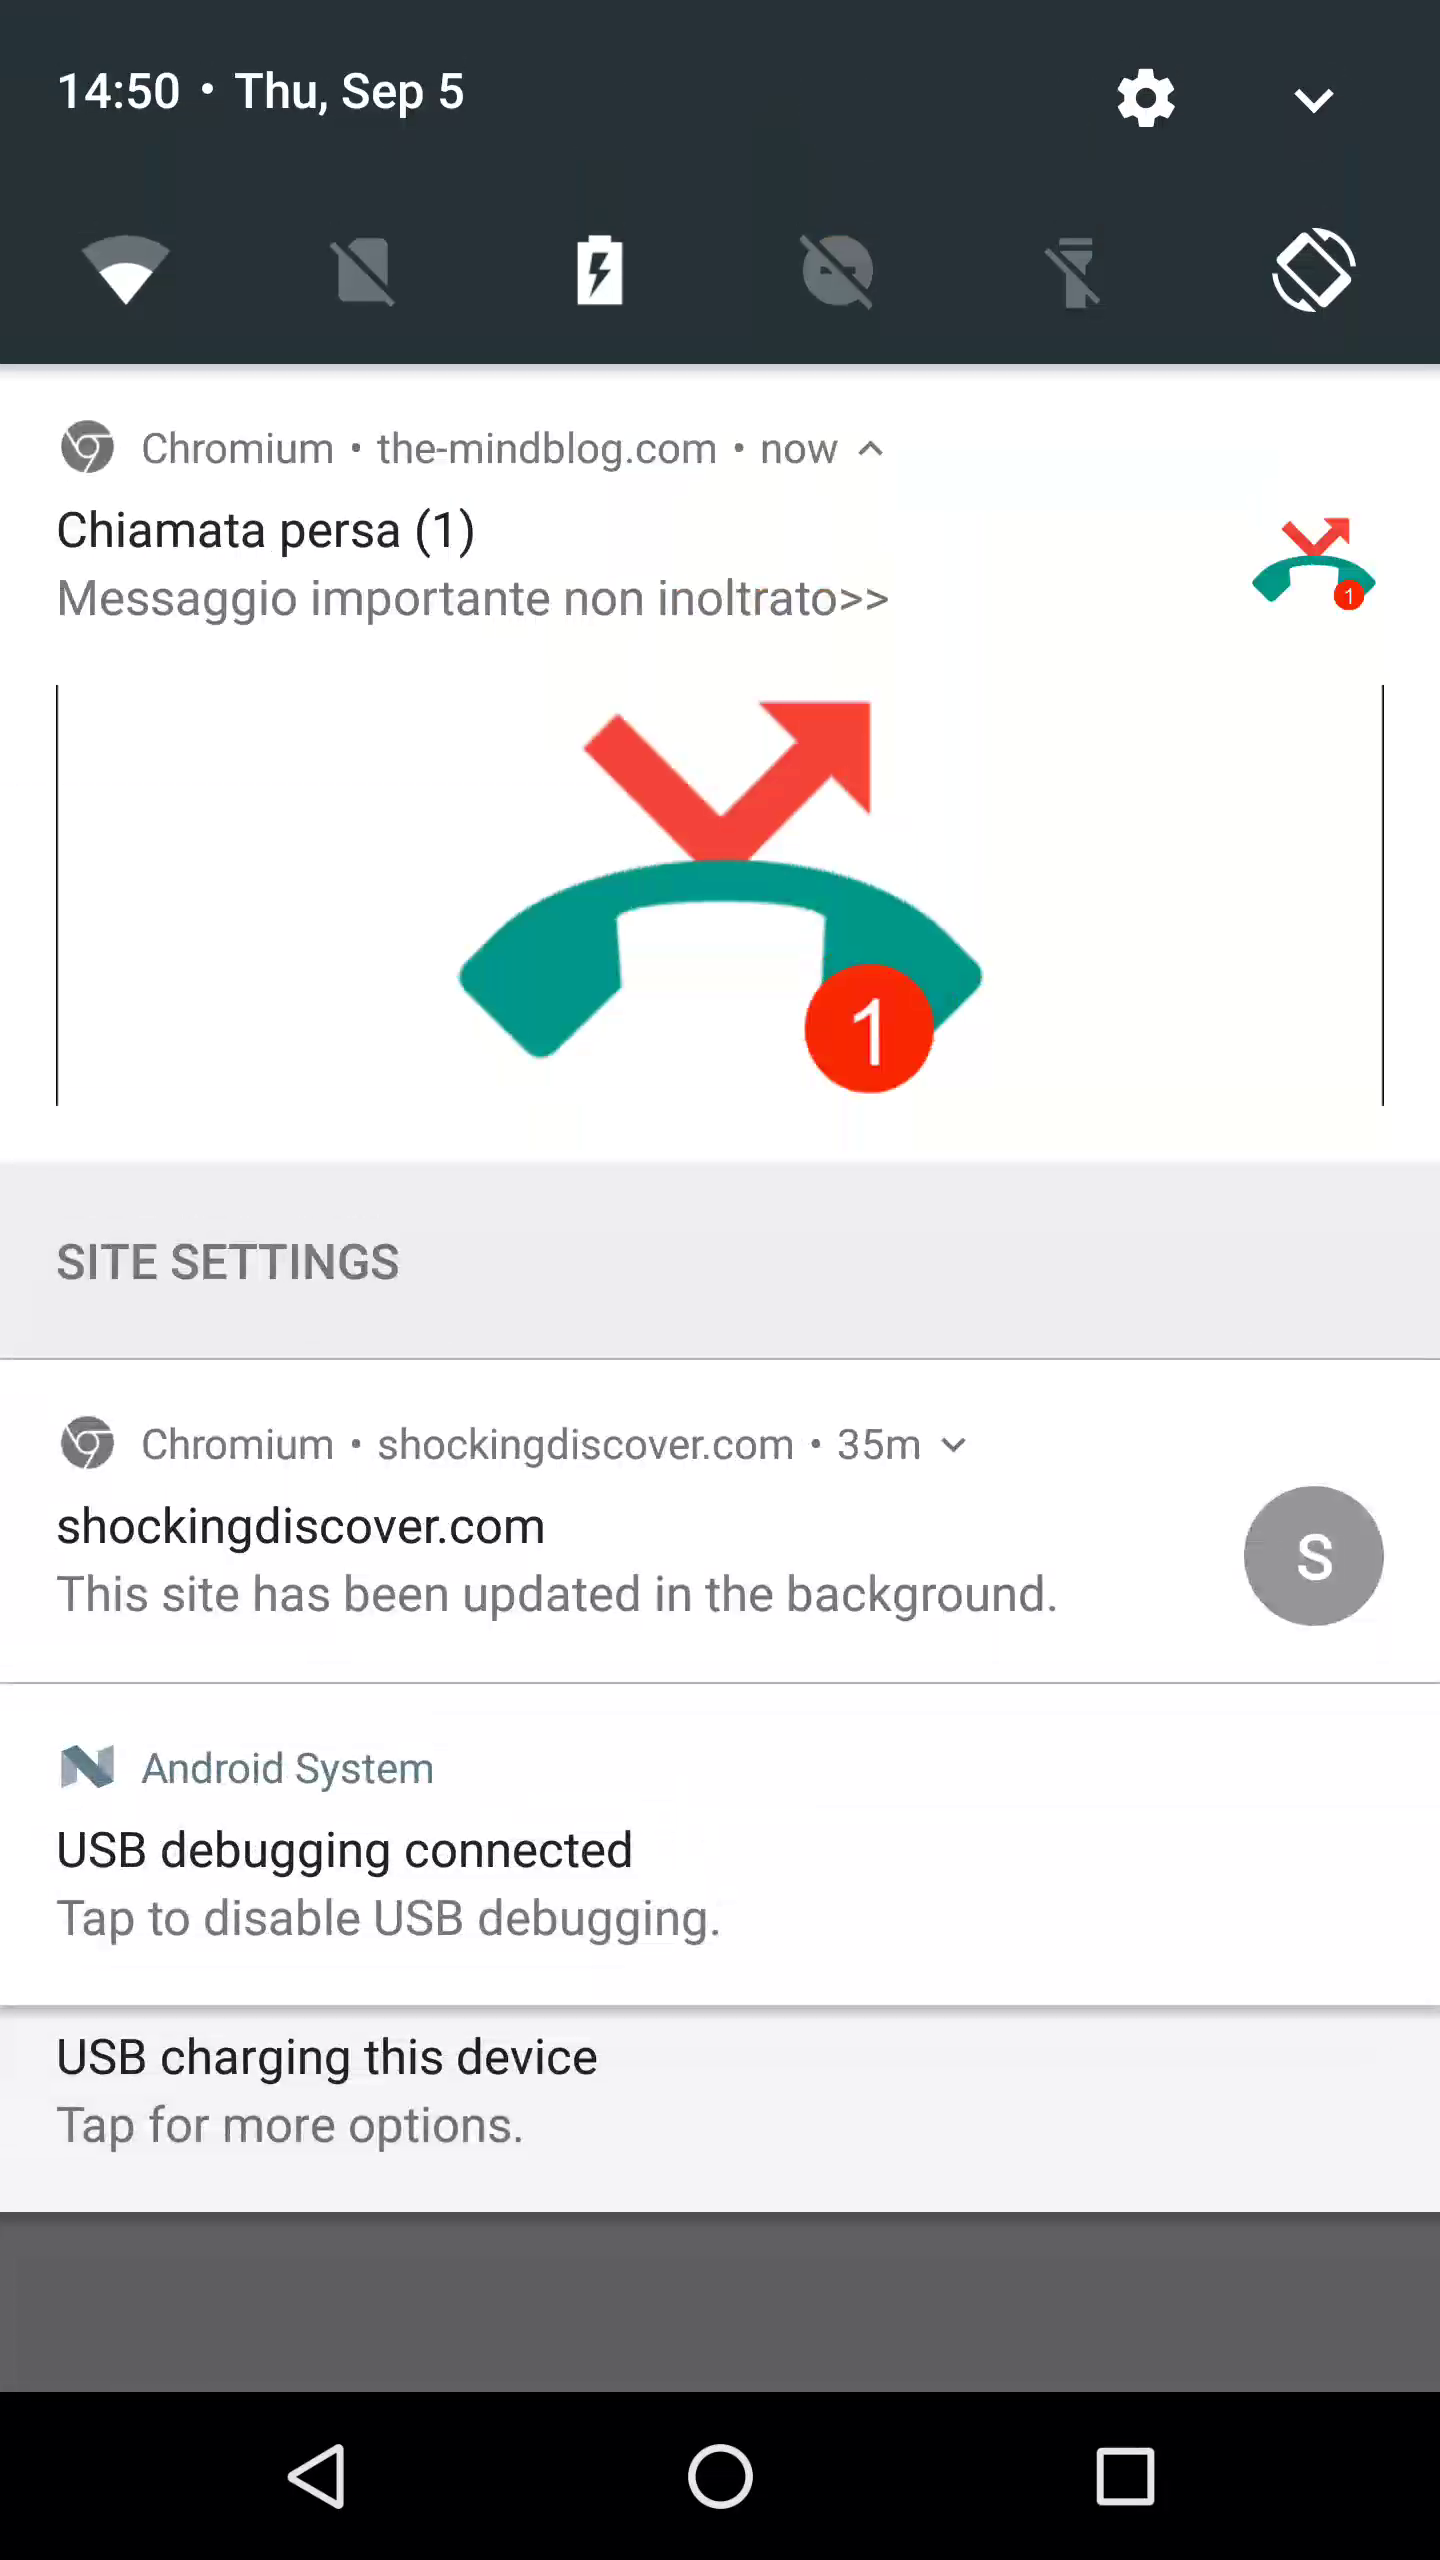
\includegraphics[scale=0.06]{figs/mobile_1}
        \caption{}
    \end{center}
    \end{subfigure}
   \begin{subfigure}{.18\textwidth} 
    \begin{center}
        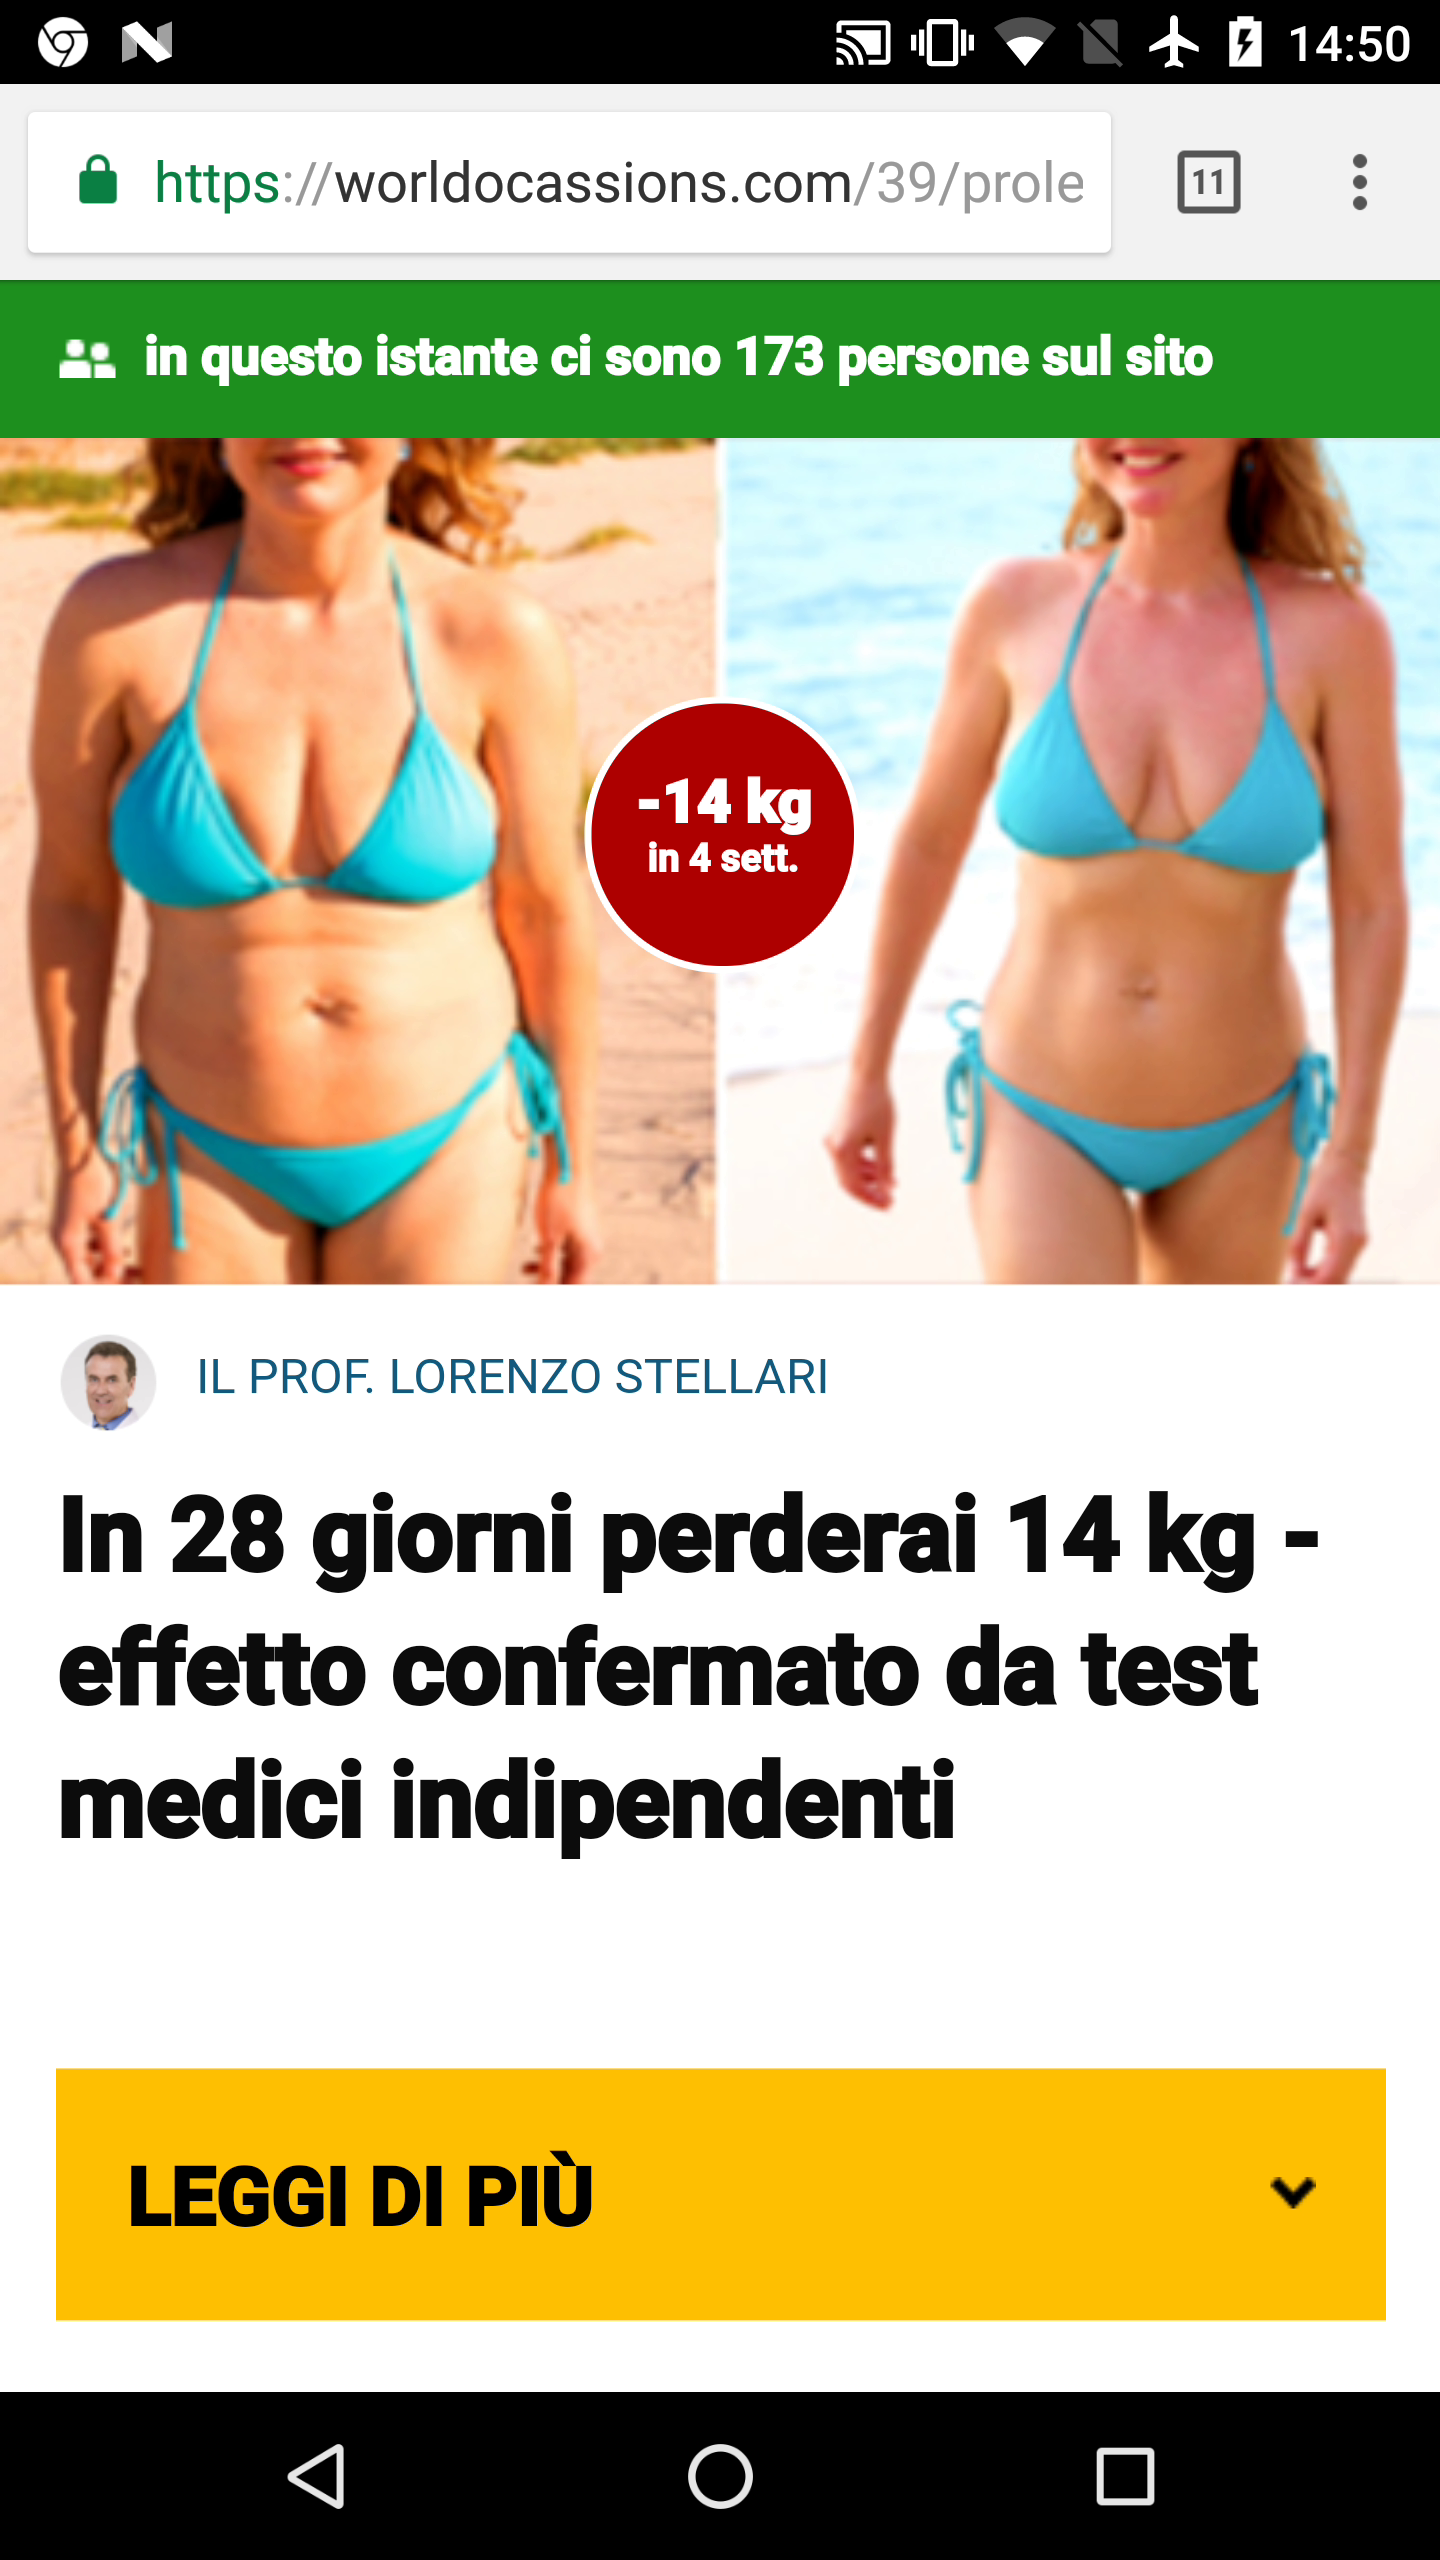
\includegraphics[scale=0.06]{figs/mobile_2}
        \caption{}
    \end{center}
    \end{subfigure}
    \begin{subfigure}{.18\textwidth}
    \begin{center}
        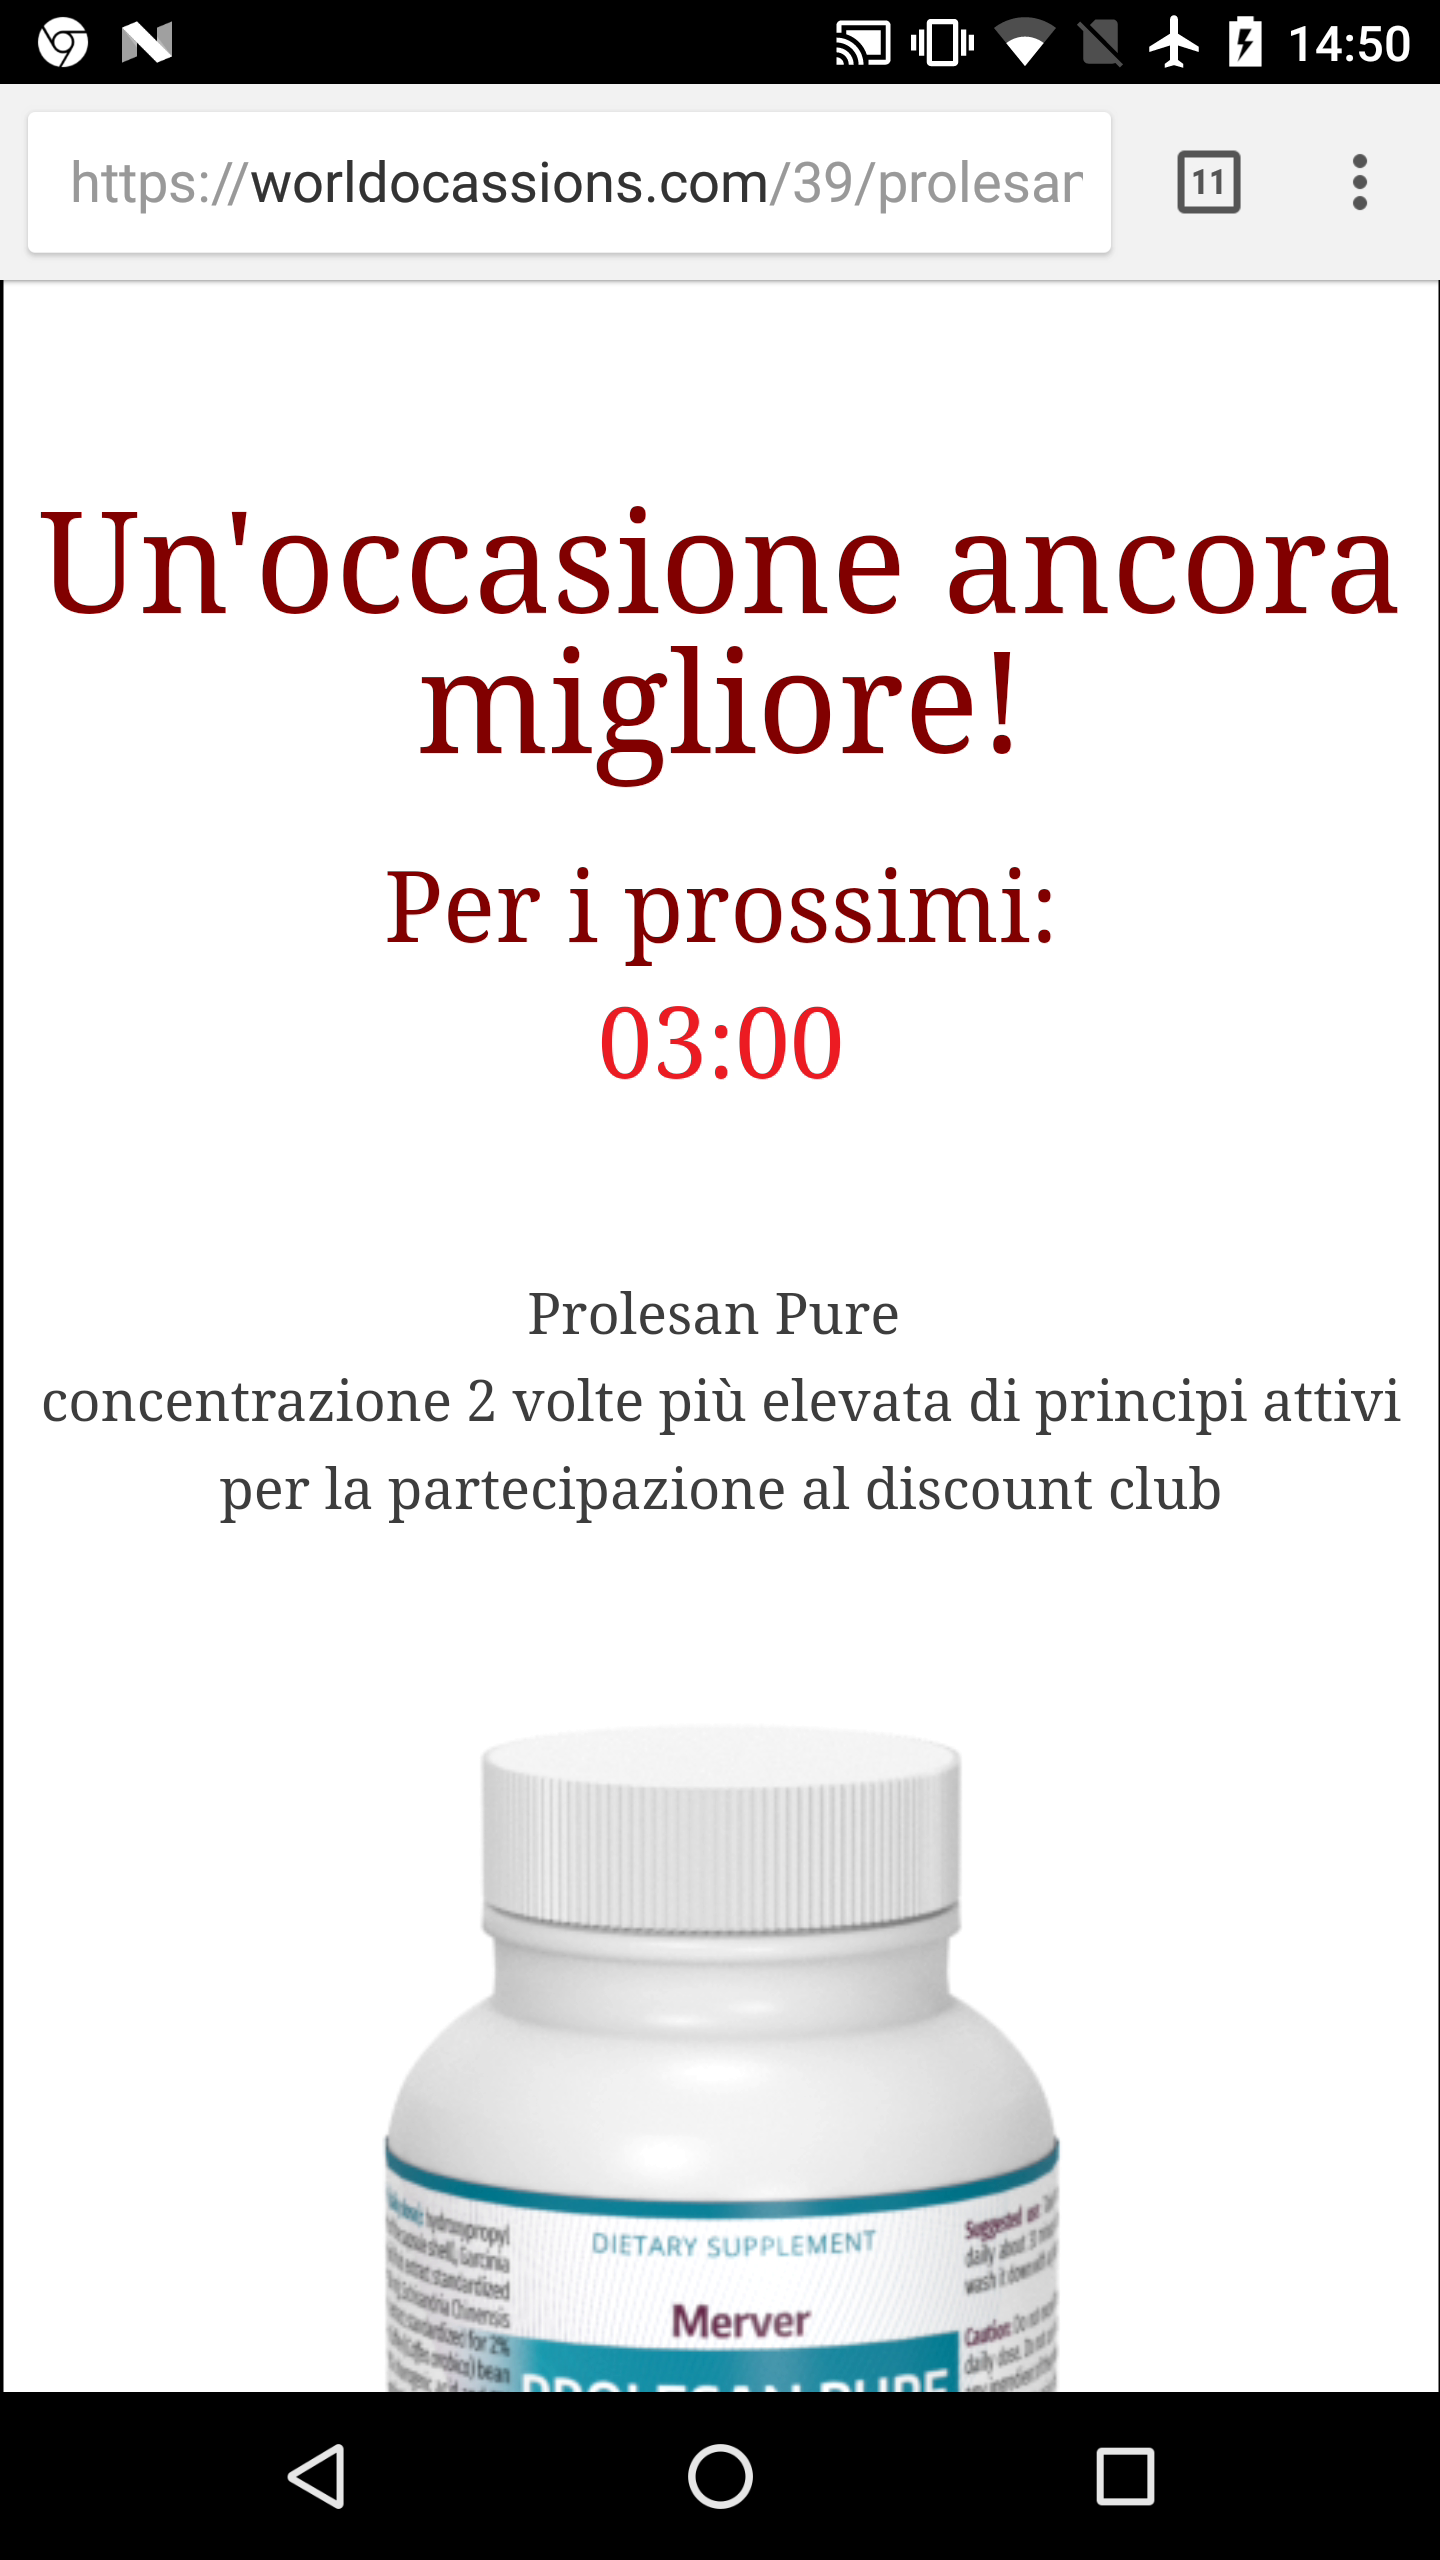
\includegraphics[scale=0.06]{figs/mobile_3}
        \caption{}
    \end{center}
    \end{subfigure}
    \begin{subfigure}{.18\textwidth}
    \begin{center}
        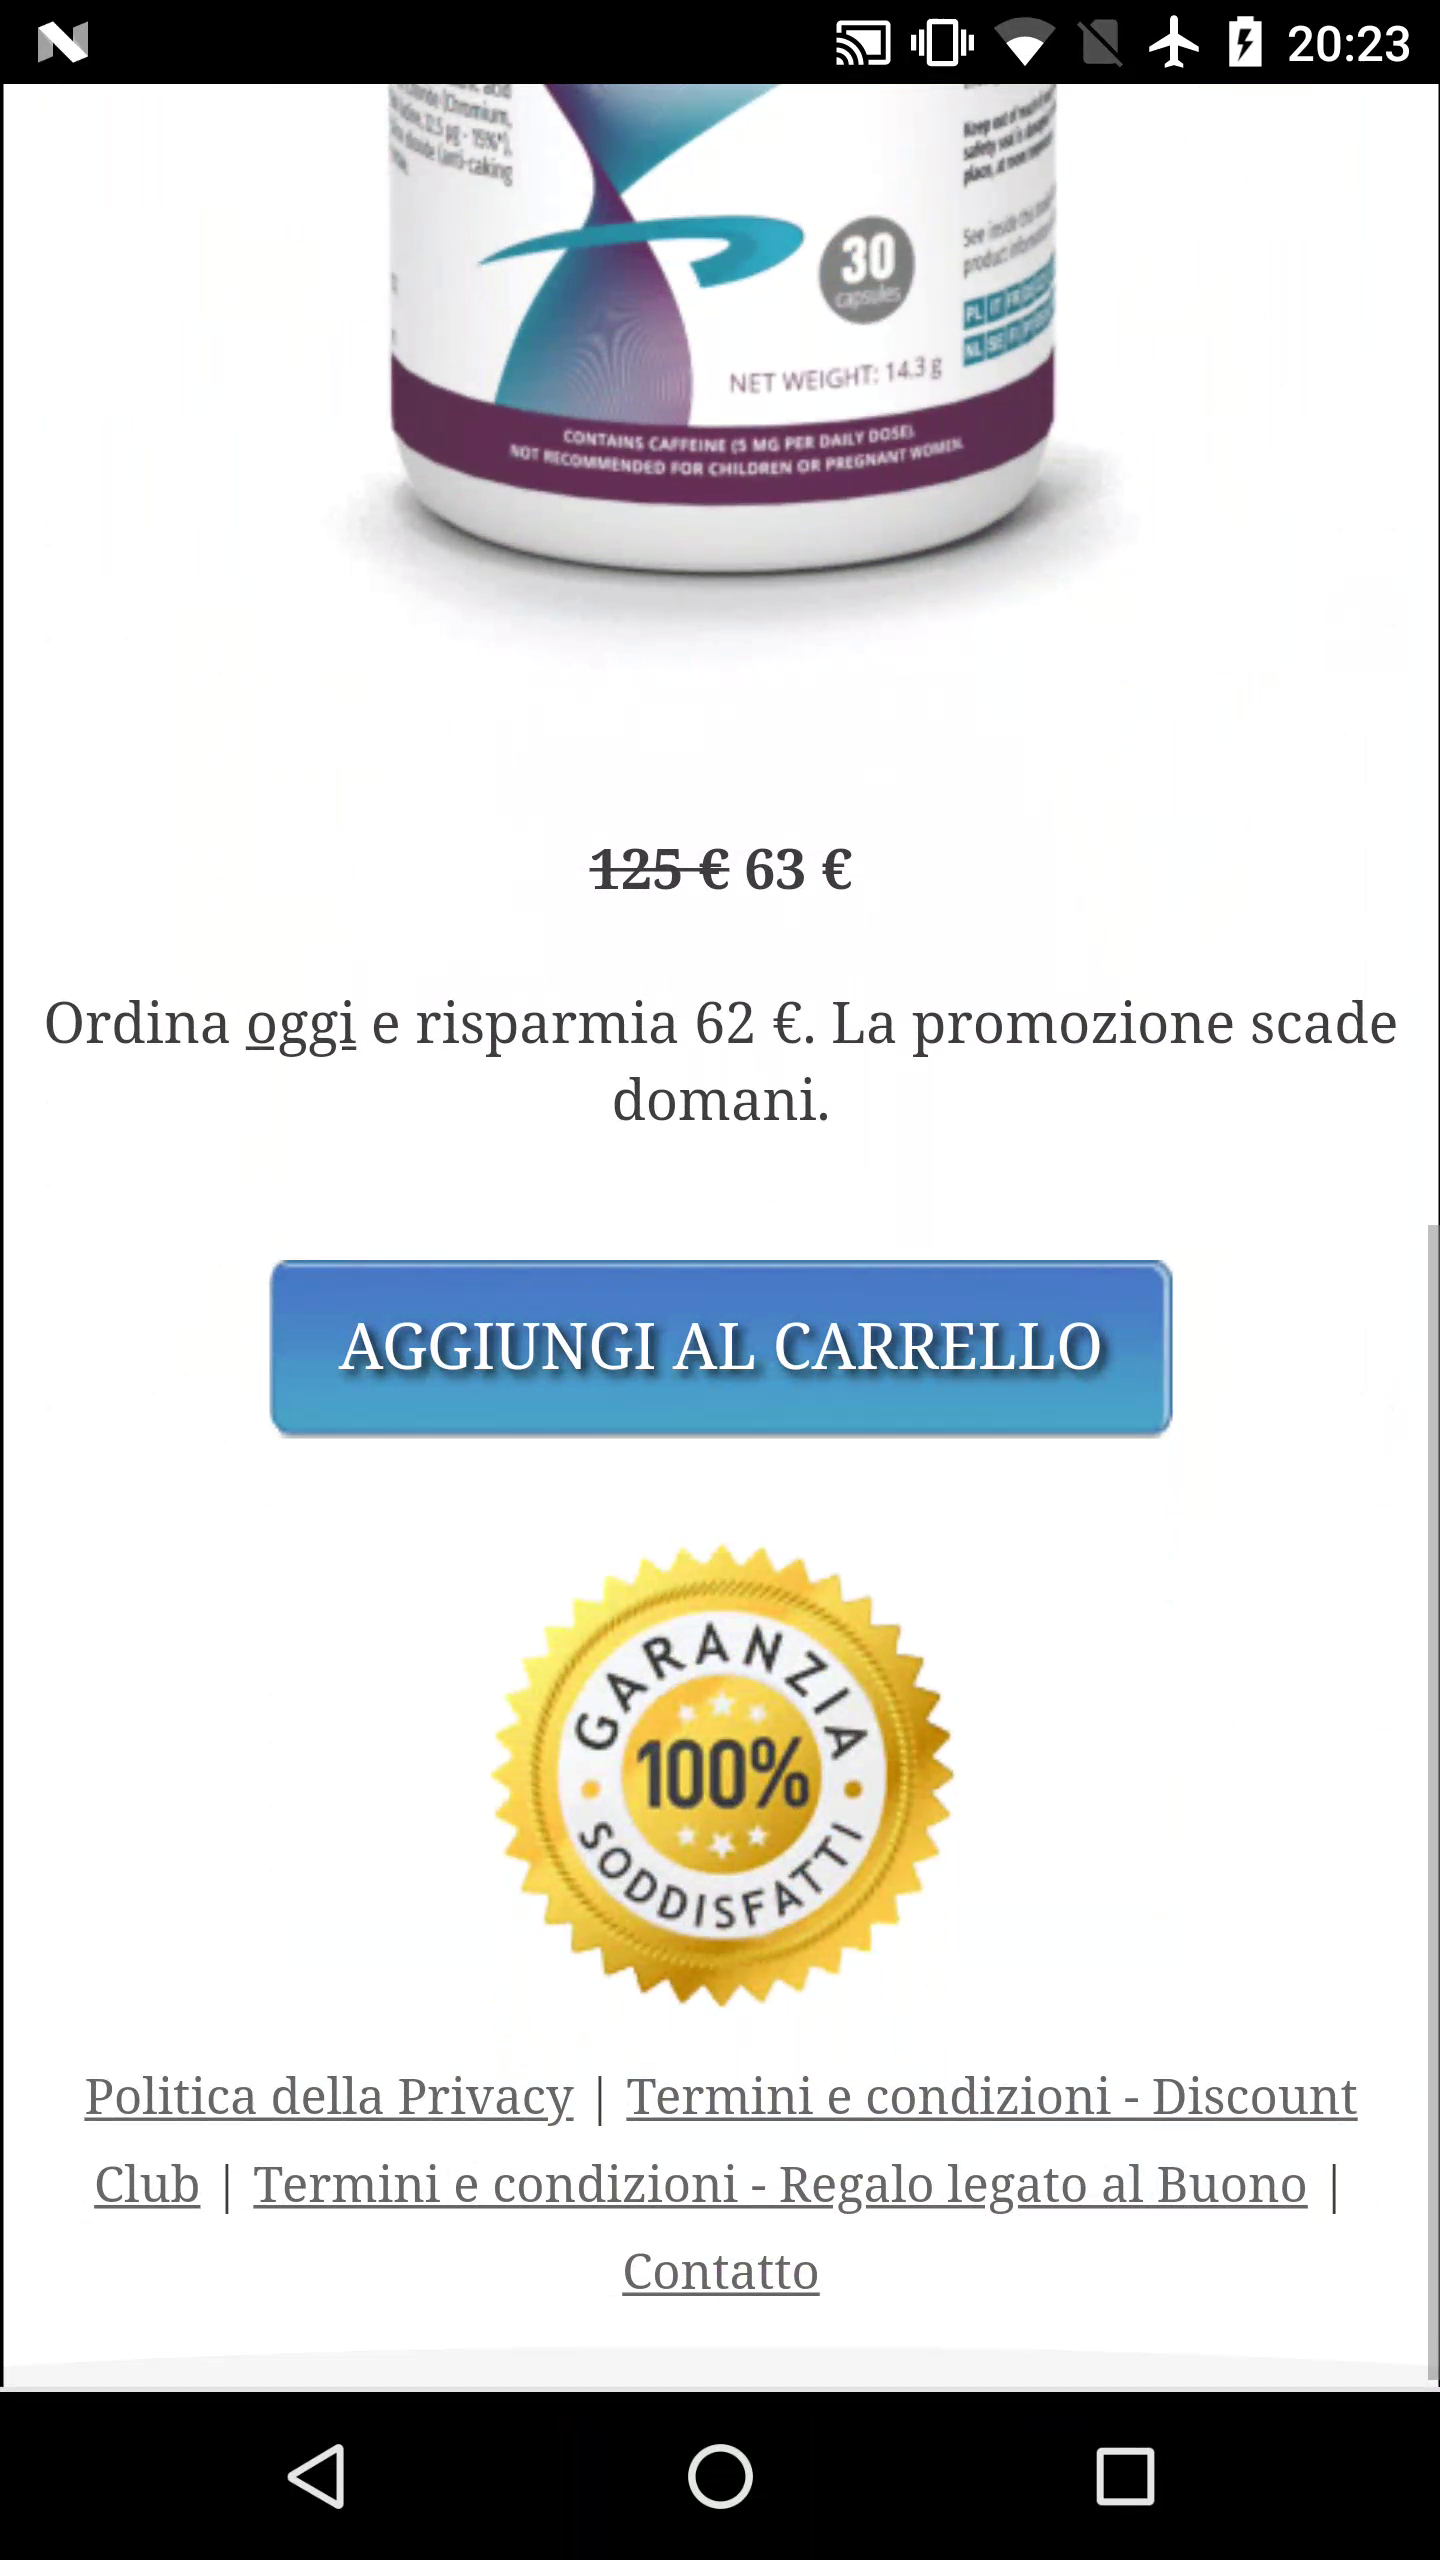
\includegraphics[scale=0.06]{figs/mobile_4}
        \caption{}
    \end{center}
    \end{subfigure}
    \begin{subfigure}{.18\textwidth} 
    \begin{center}
        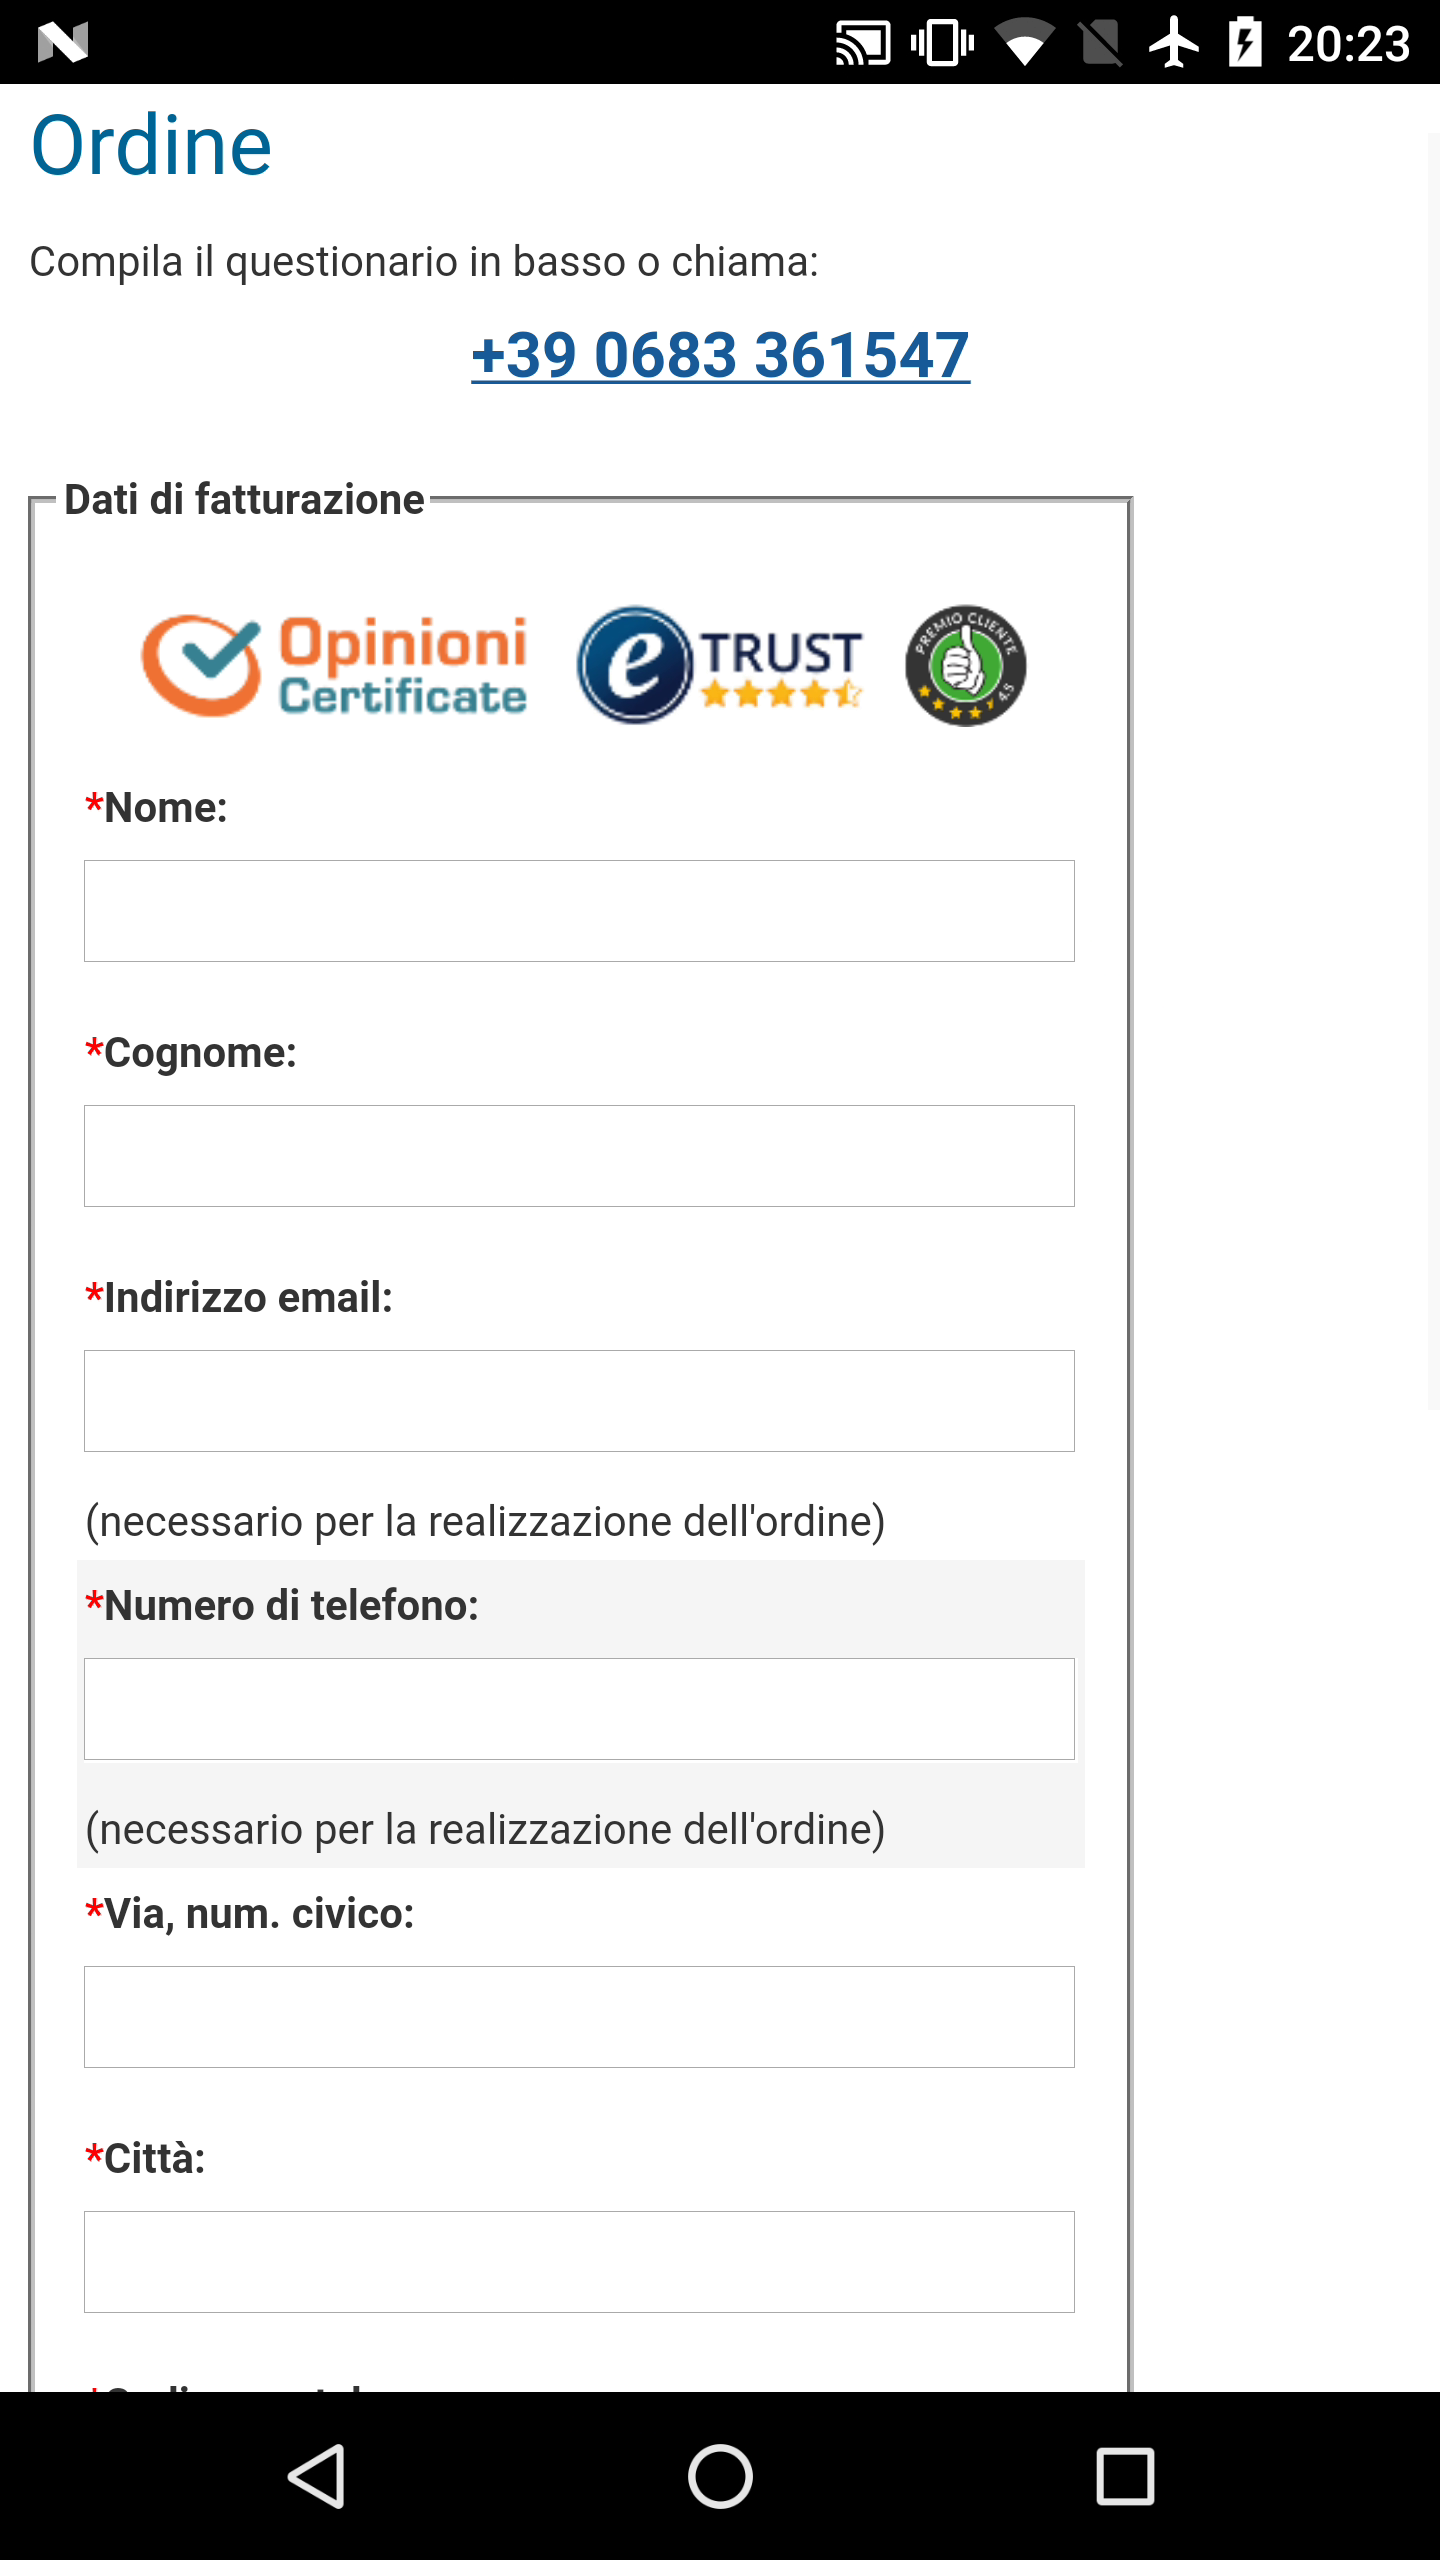
\includegraphics[scale=0.06]{figs/mobile_5}
        \caption{}
    \end{center}
    \end{subfigure}
    
    \caption{Mobile Case Study (a)Displays Notification of a 'Missed Call' (b)Initial Landing Page after clicking the notification displays article on weight loss (c) Redirected Page (d) Redirected Page-contd. (e)Displays a form collecting sensitive information }
    \label{fig:mobile}
\end{center}
\end{figure*}



% \begin{figure}[h]
% \begin{center}
%     \begin{subfigure}{.24\textwidth}
%     \begin{center}
%         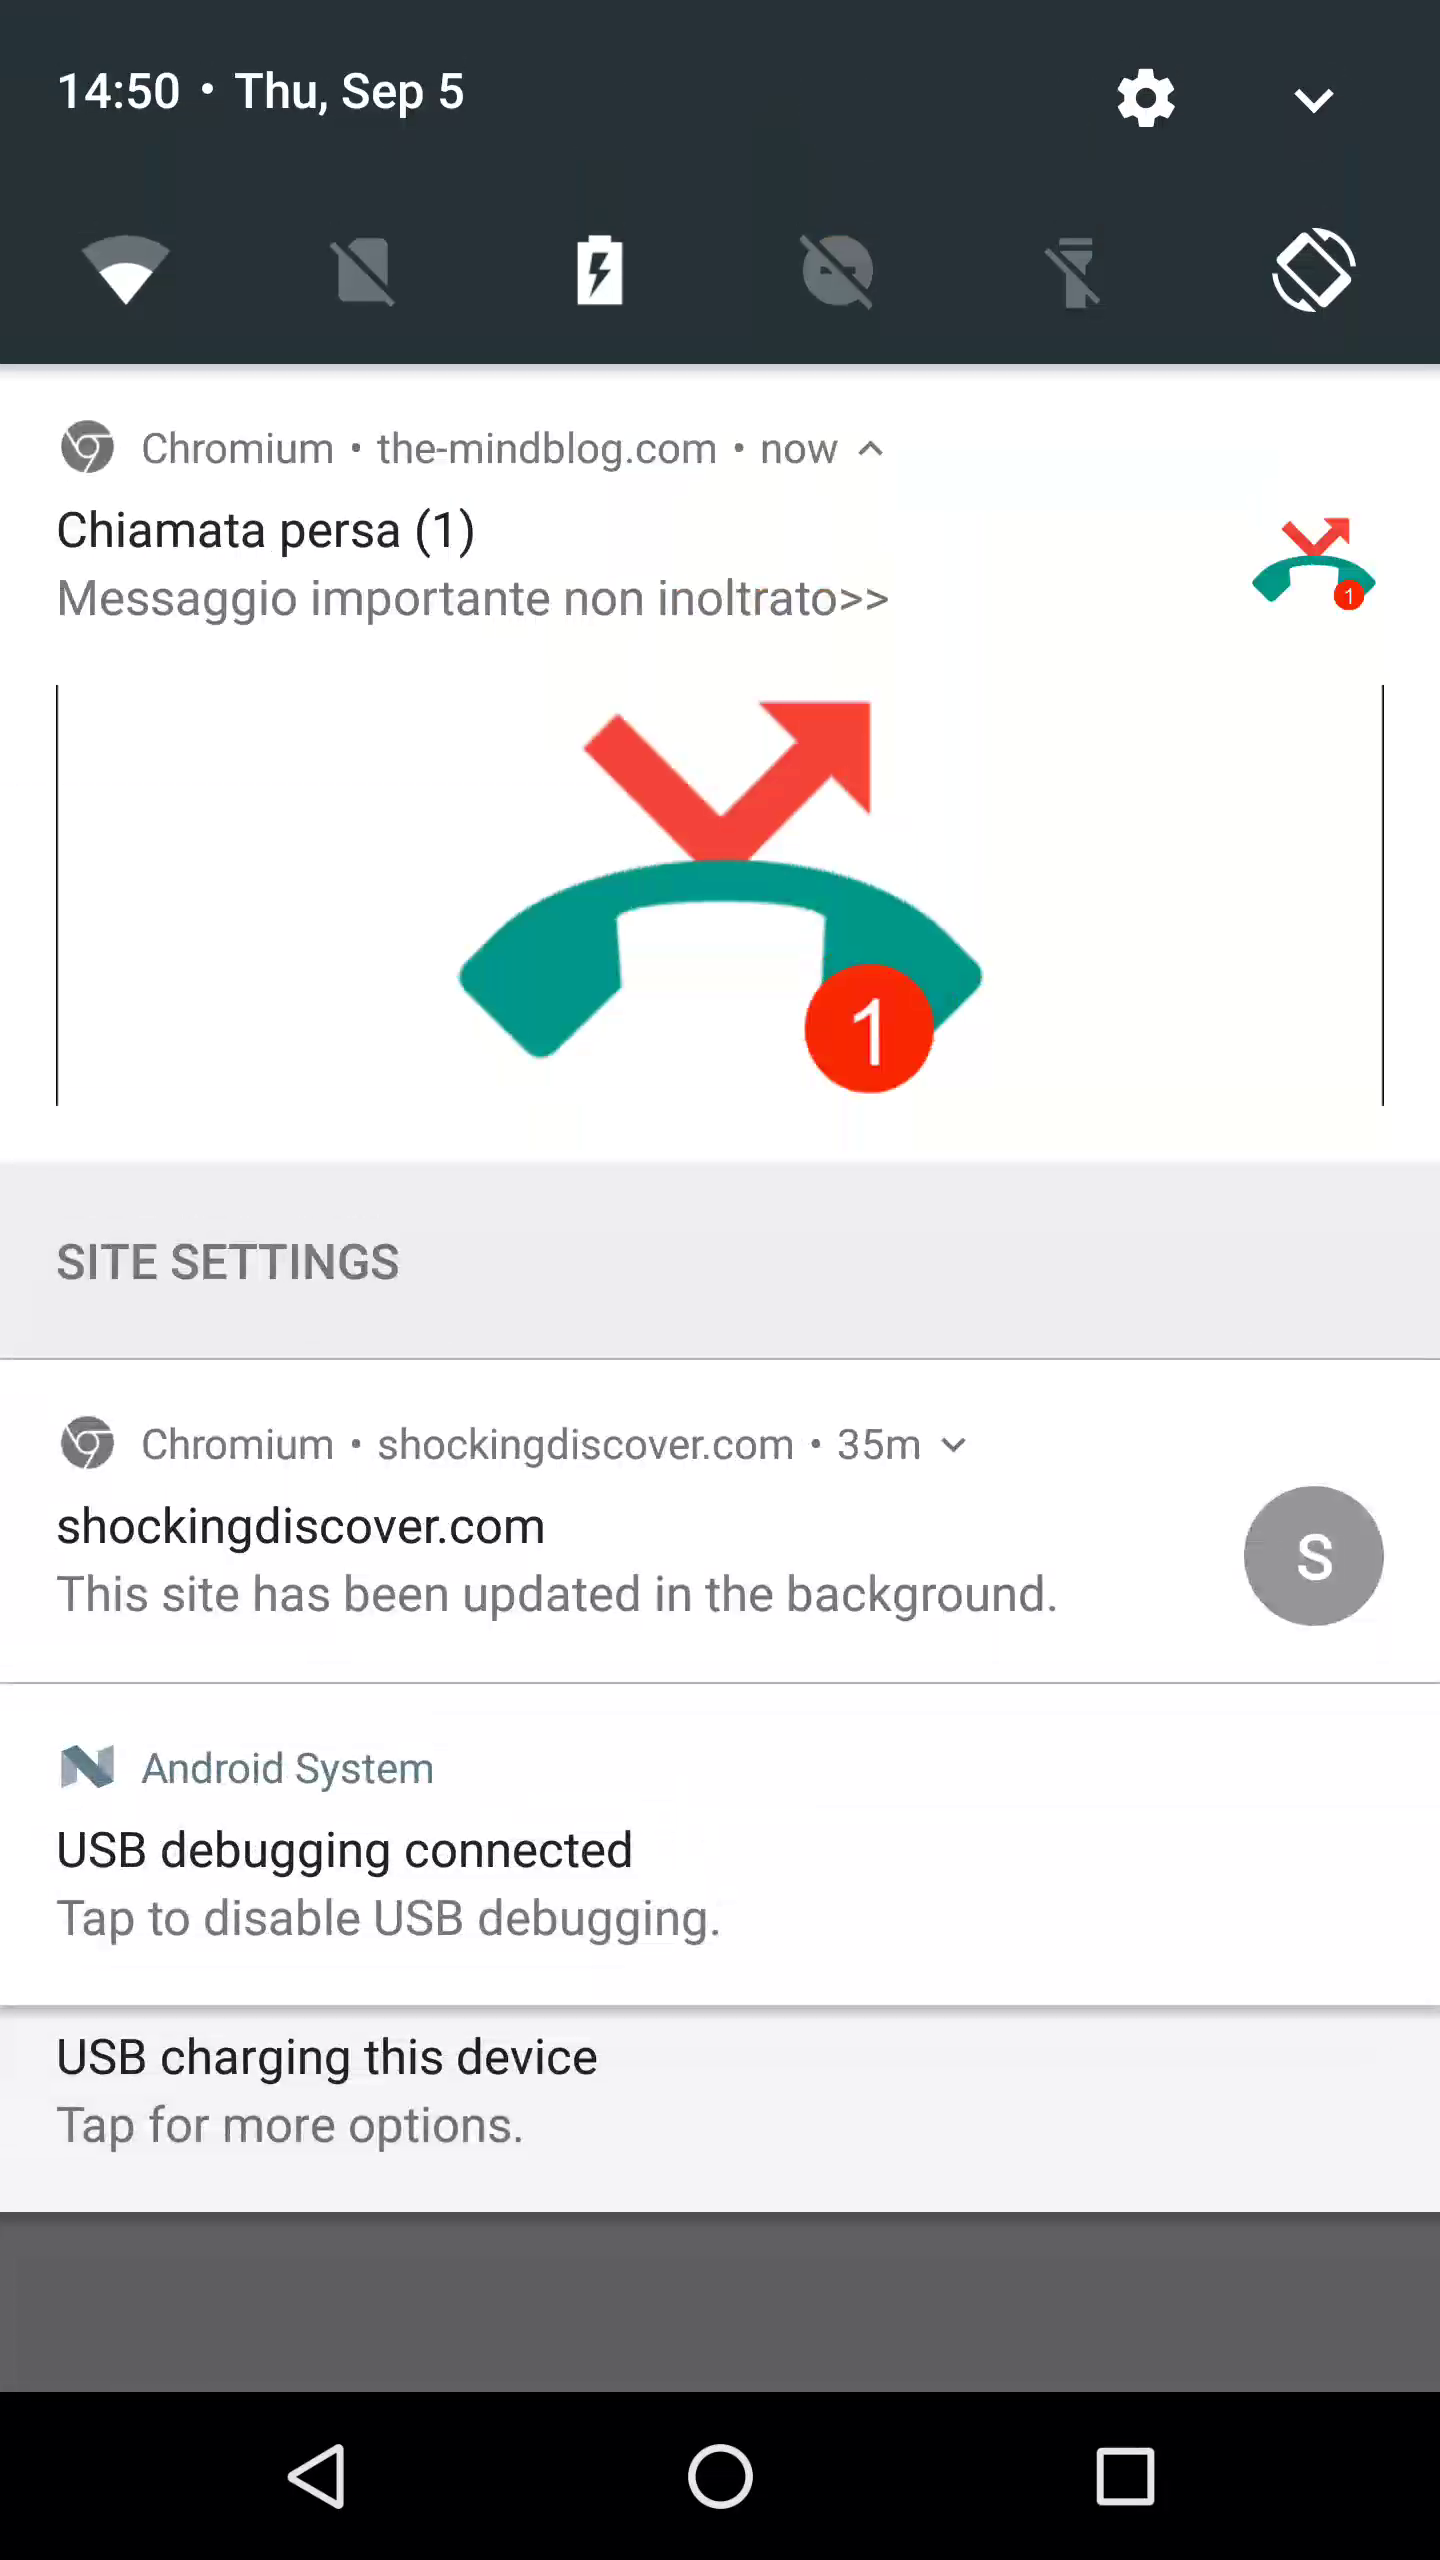
\includegraphics[scale=0.08]{figs/mobile_1}
%         \caption{Notification}
%     \end{center}
%     \end{subfigure}
%     \begin{subfigure}{.24\textwidth} 
%     \begin{center}
%         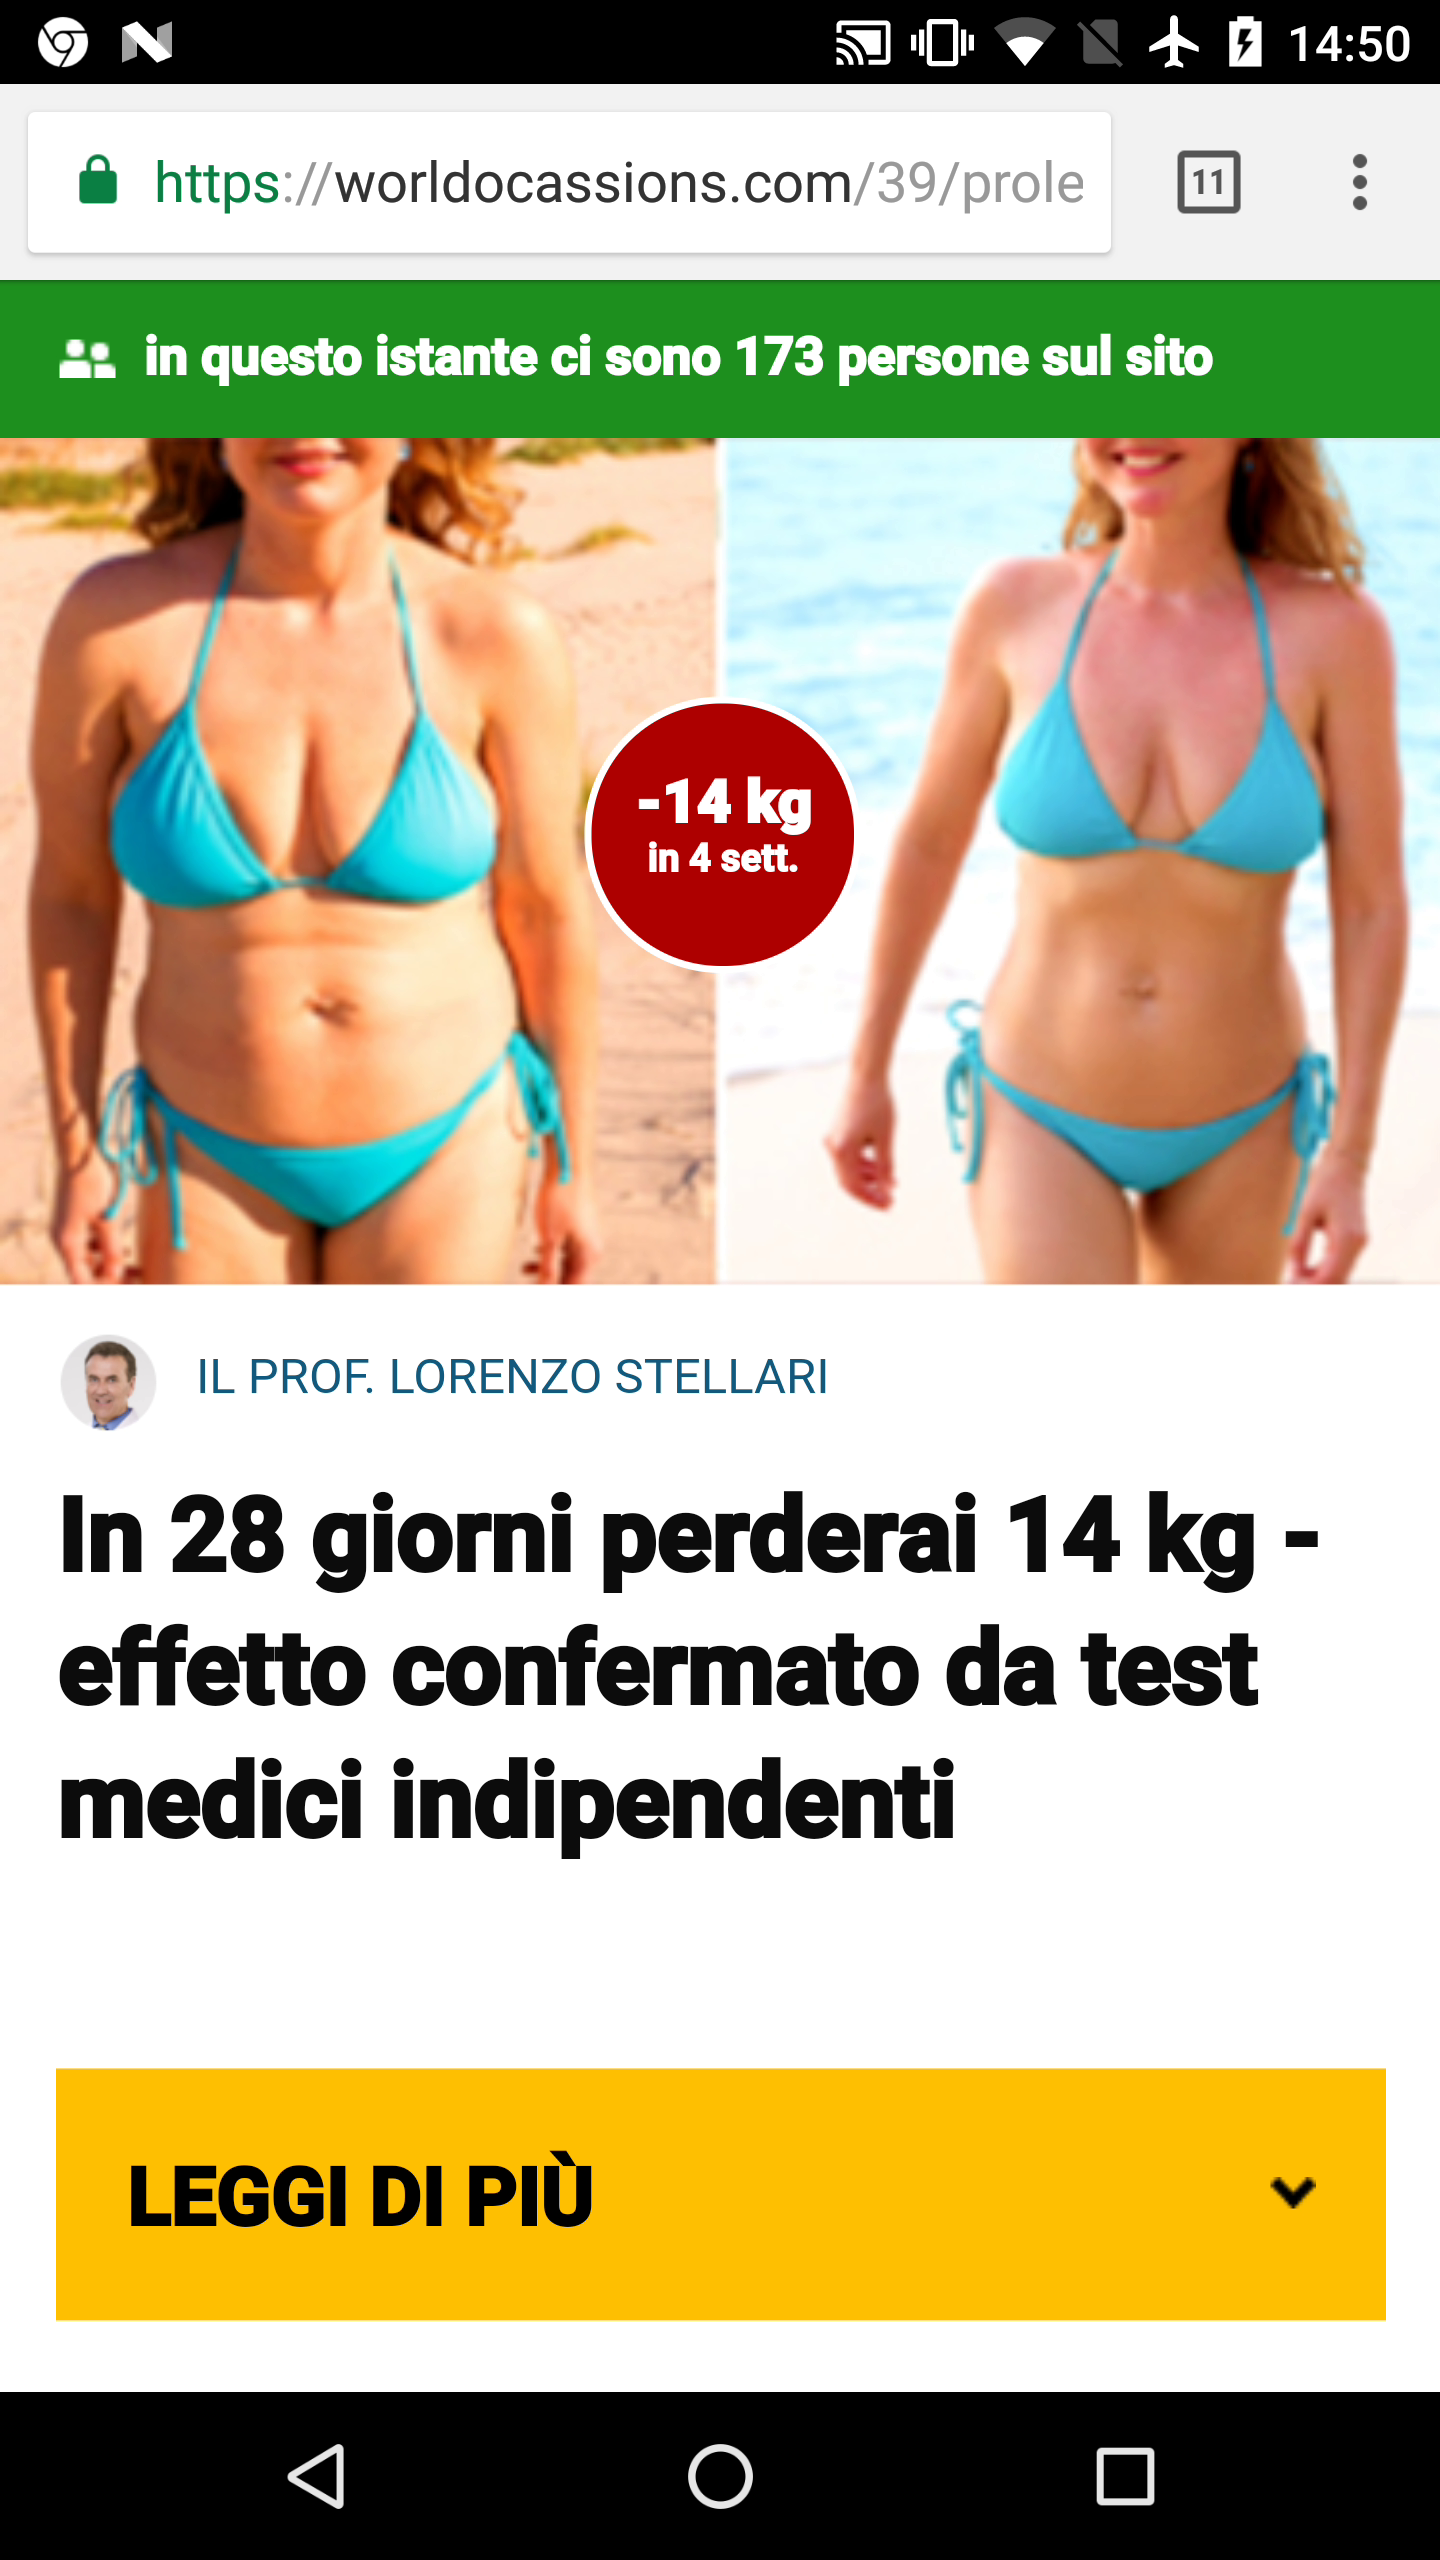
\includegraphics[scale=0.08]{figs/mobile_2}
%         \caption{Initial Landing Page}
%     \end{center}
%     \end{subfigure}
%     \begin{subfigure}{.24\textwidth} 
%     \begin{center}
%         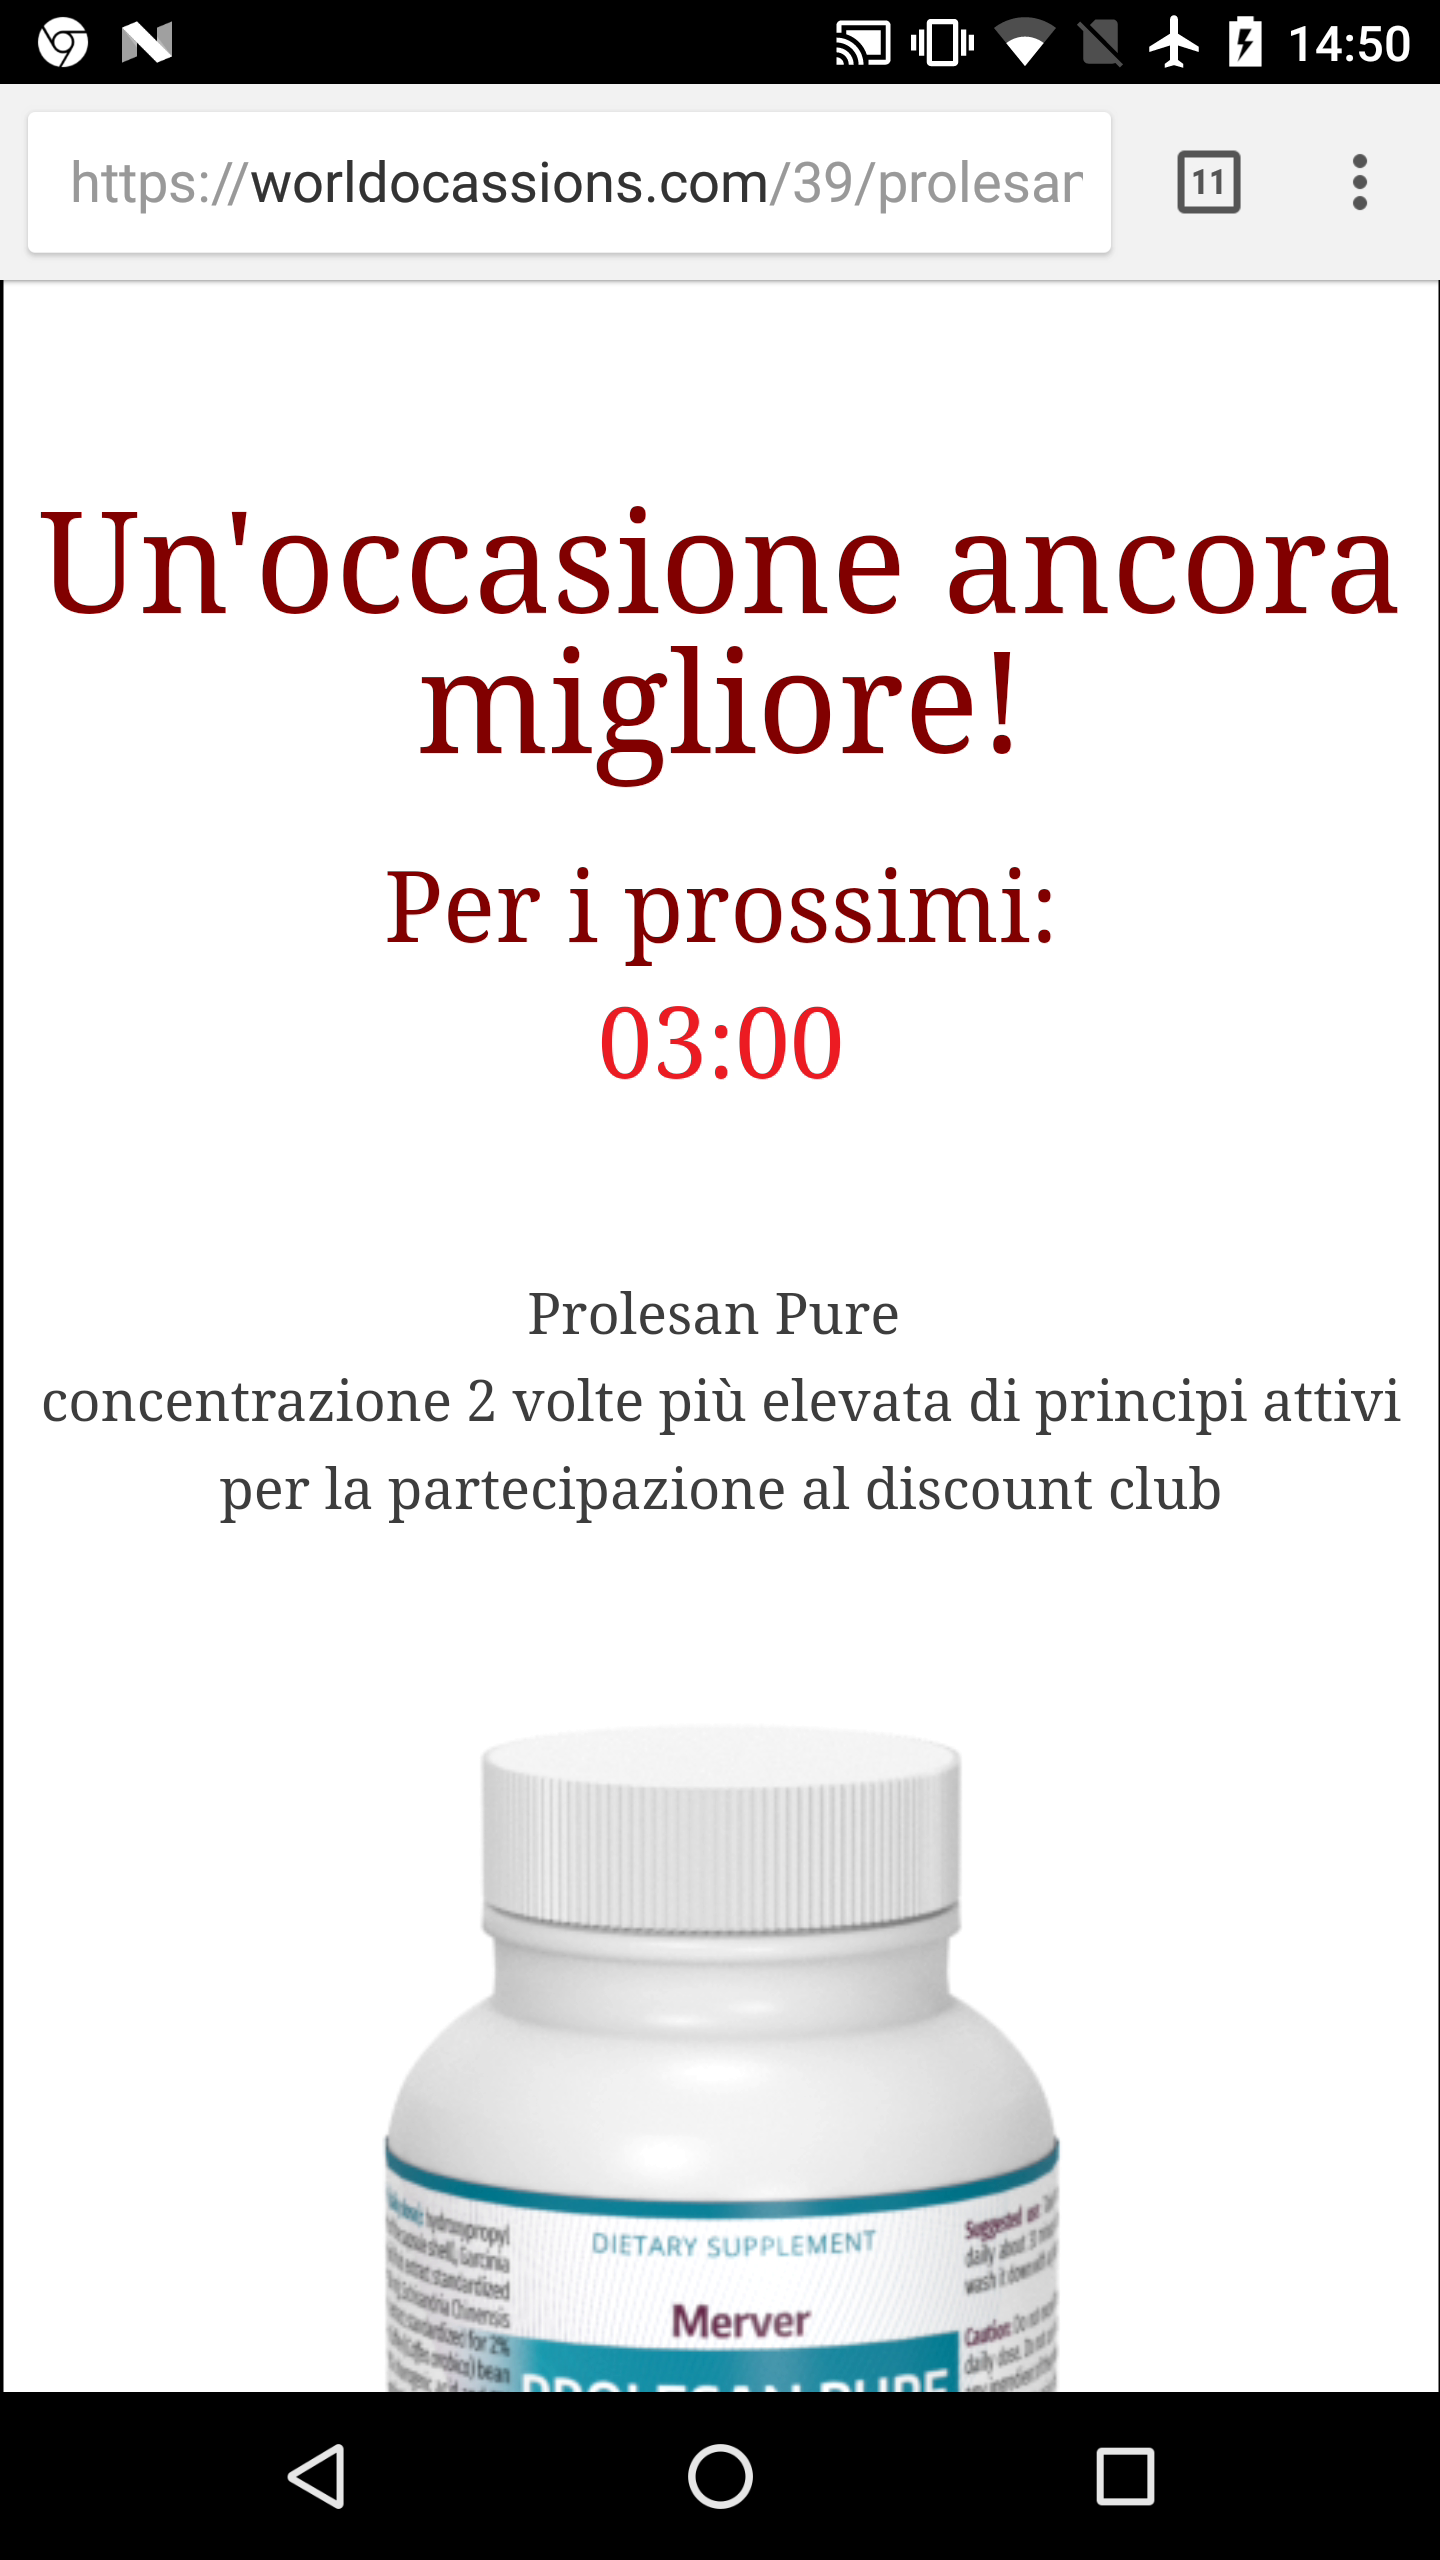
\includegraphics[scale=0.08]{figs/mobile_3}
%         \caption{Redirected Page}
%     \end{center}
%     \end{subfigure}
%     \begin{subfigure}{.24\textwidth} 
%     \begin{center}
%         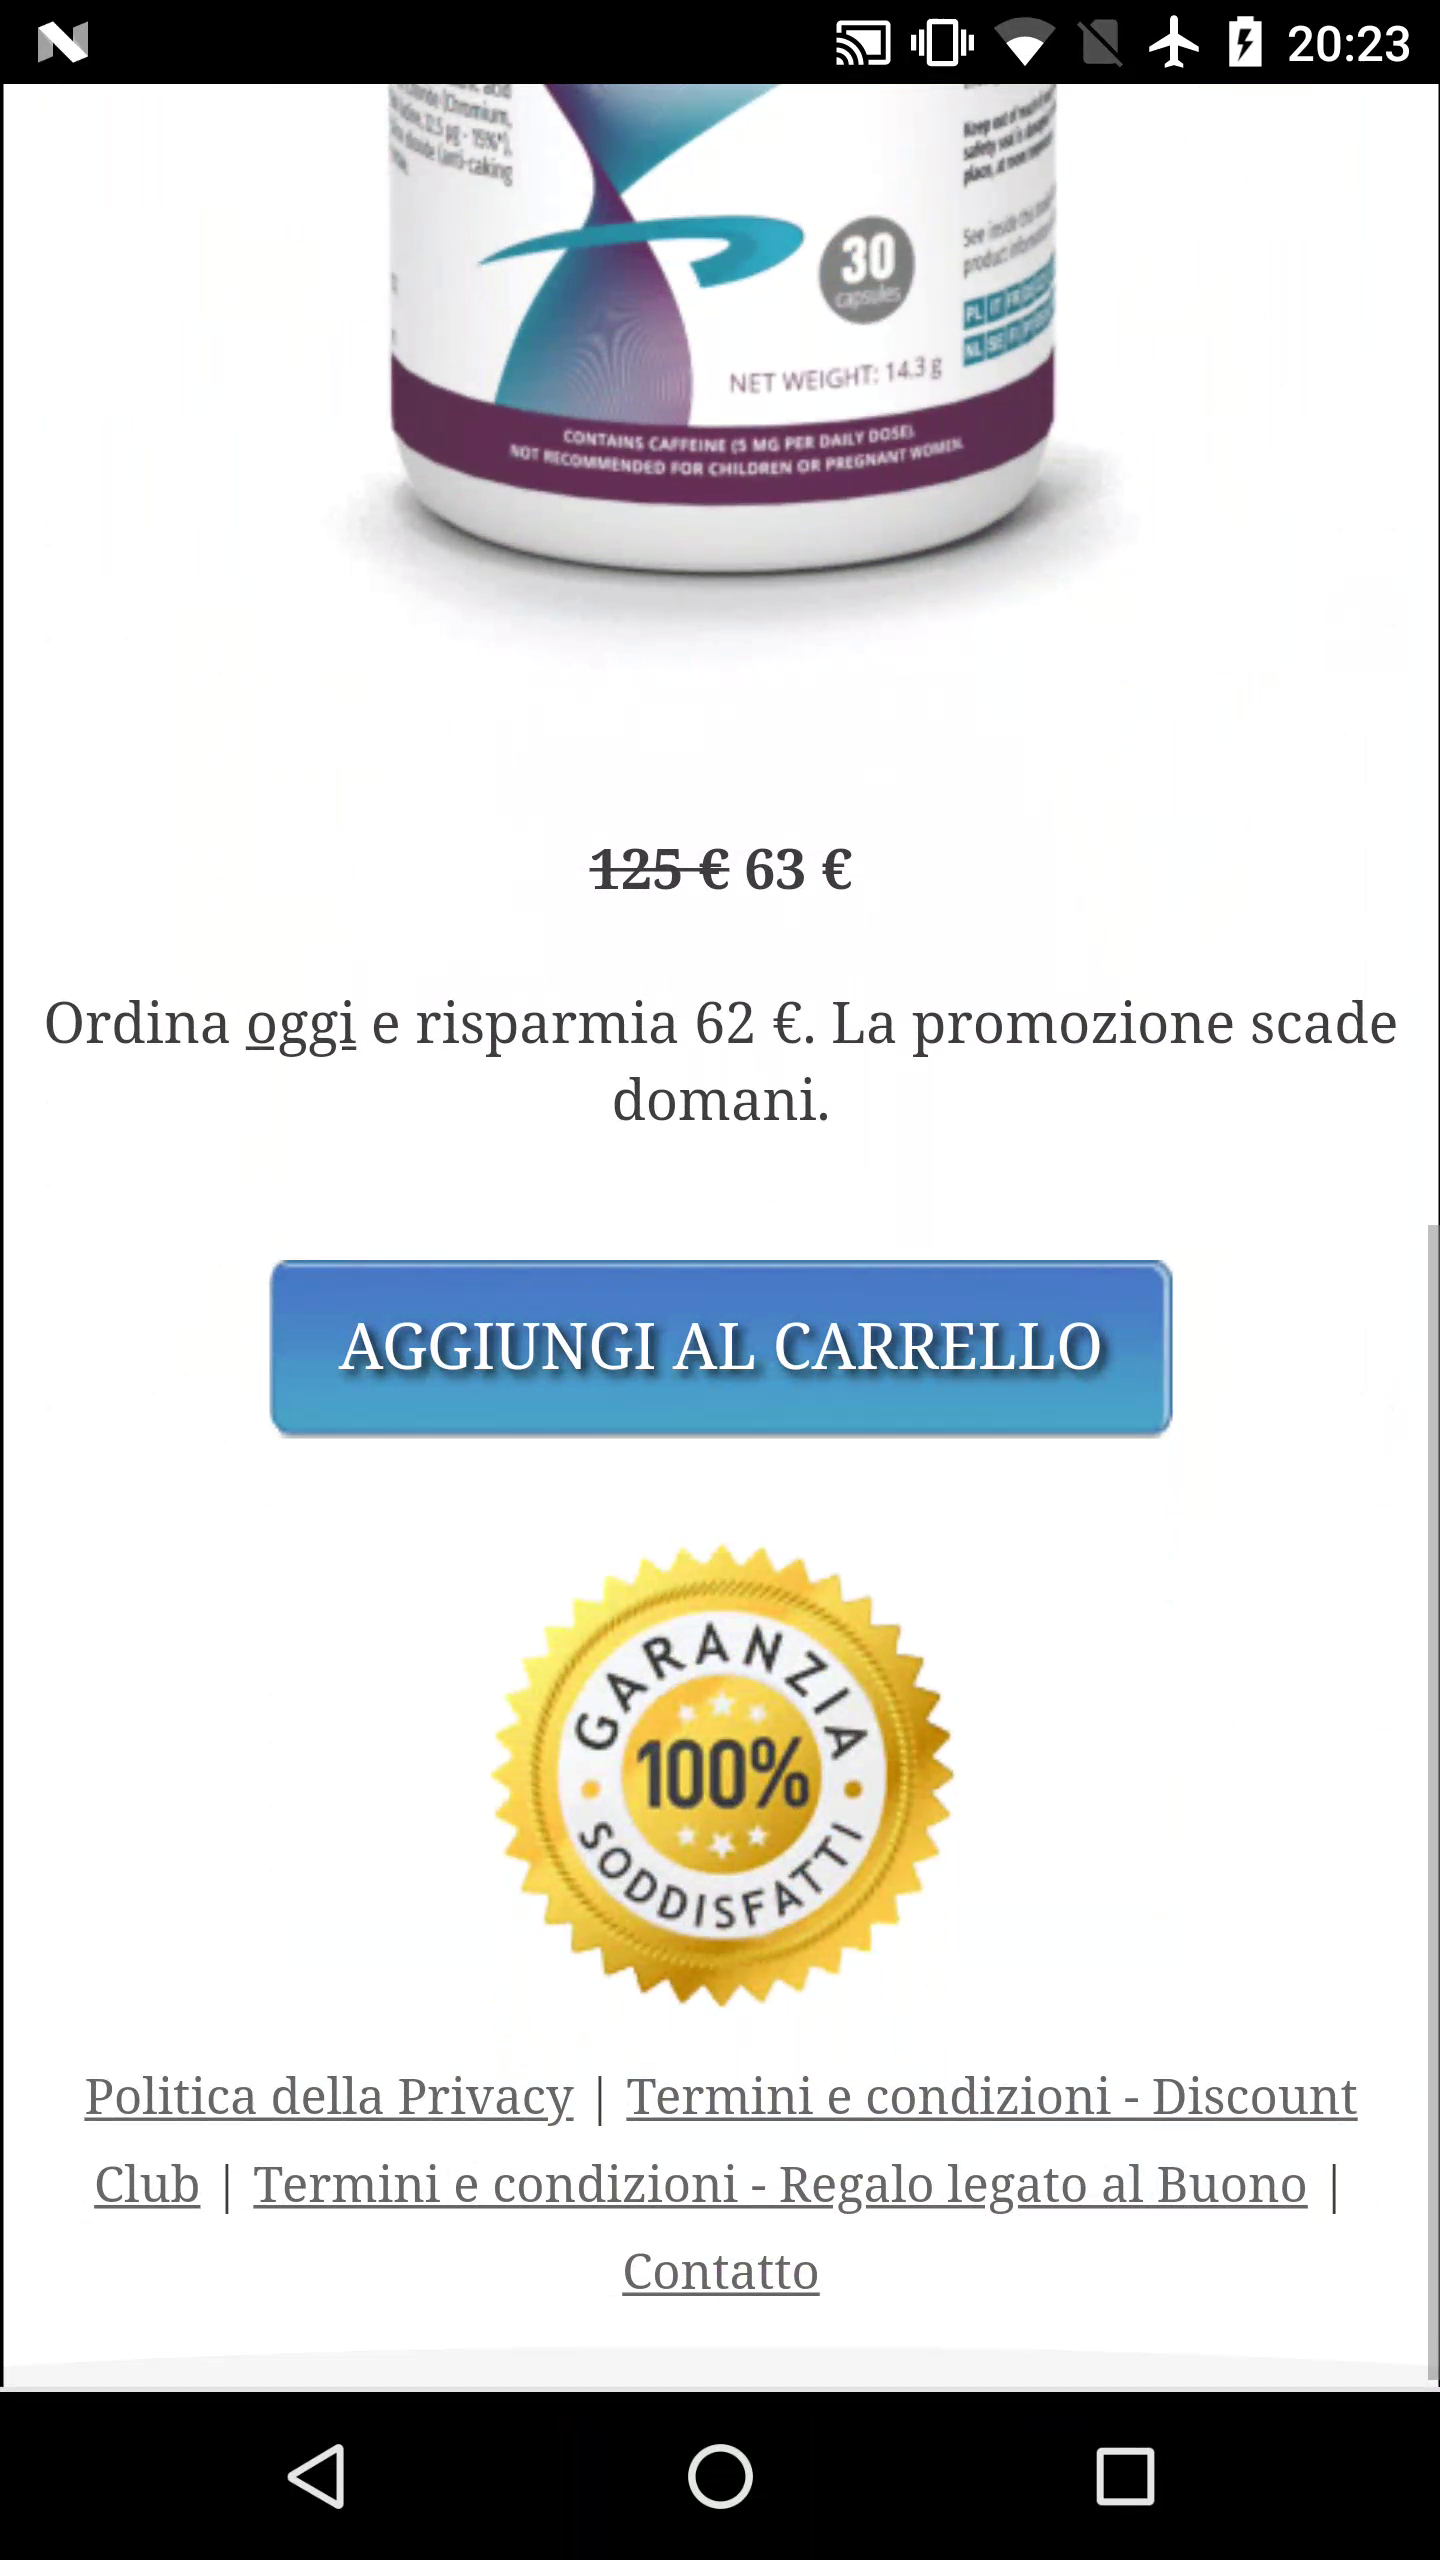
\includegraphics[scale=0.08]{figs/mobile_4}
%         \caption{Redirected Page - Cont.}
%     \end{center}
%     \end{subfigure}
%     \begin{subfigure}{.24\textwidth} 
%     \begin{center}
%         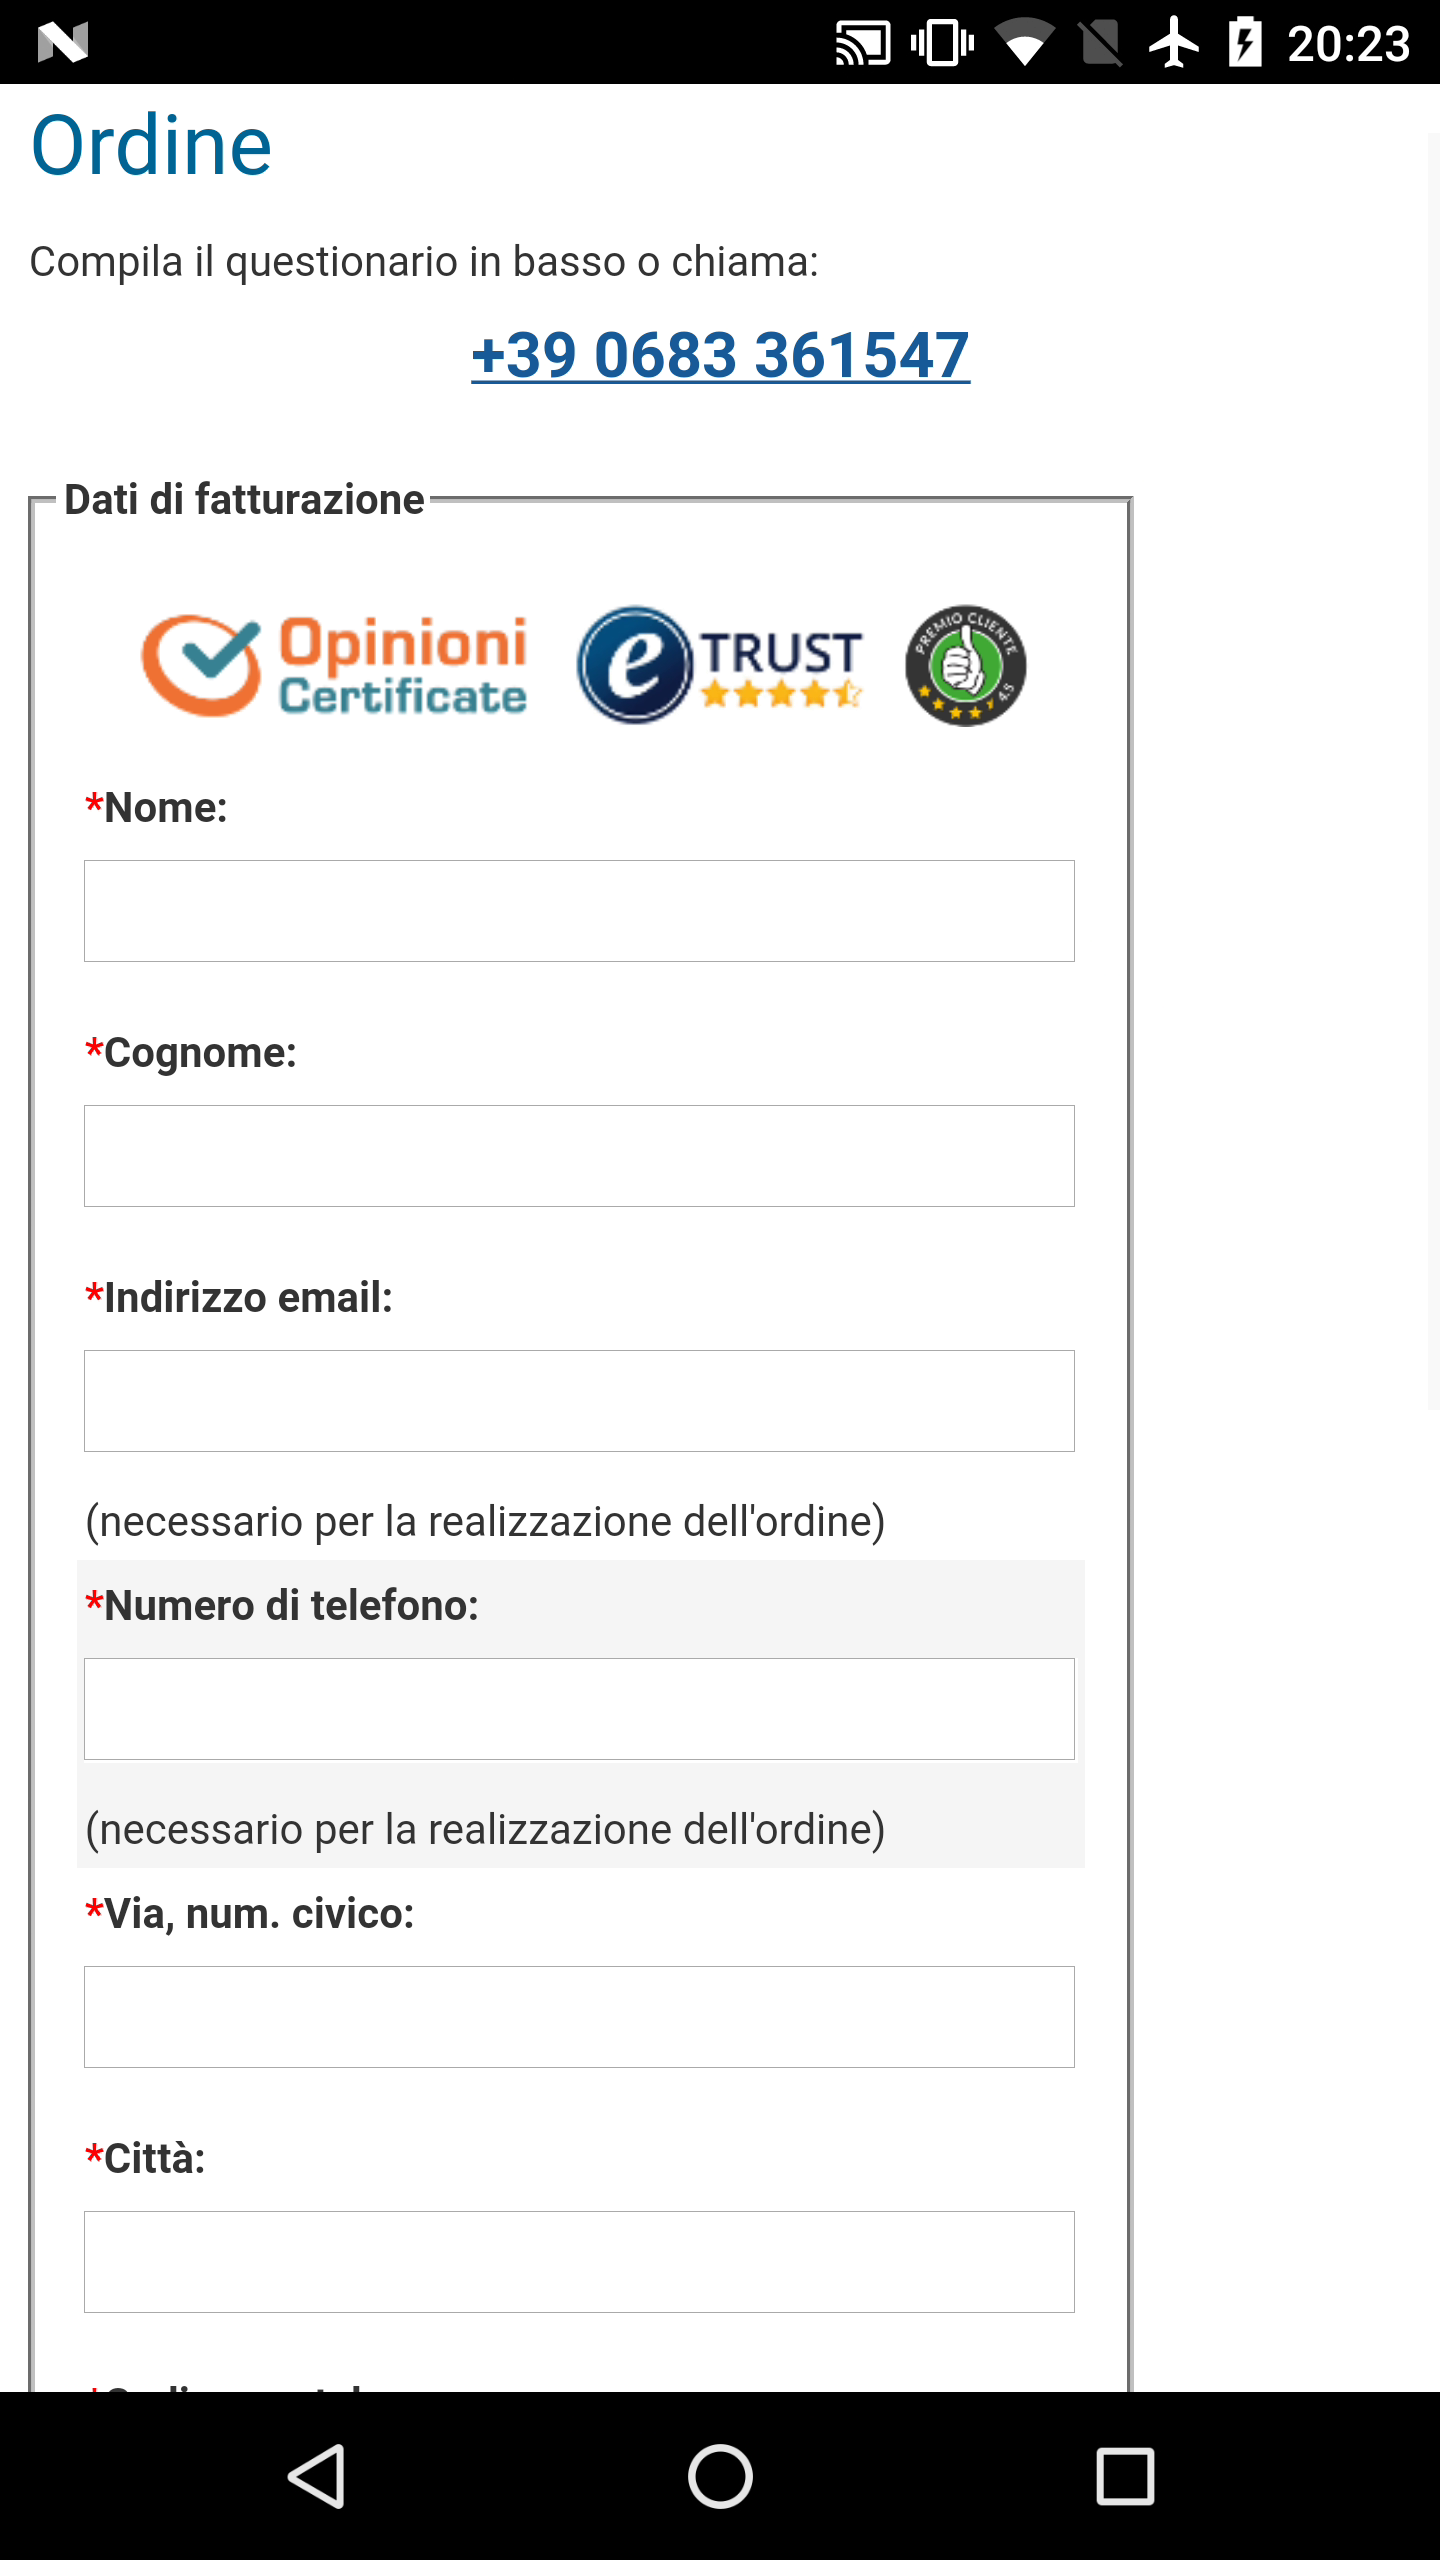
\includegraphics[scale=0.08]{figs/mobile_5}
%         \caption{Form of Sensitive Information}
%     \end{center}
%     \end{subfigure}
%     \caption{Title phishing}
%     \label{fig:mobile}
% \end{center}
% \end{figure}

% \begin{figure*}[h]
% \begin{center}
%     \begin{subfigure}{.2\textwidth}
%     \begin{center}
%         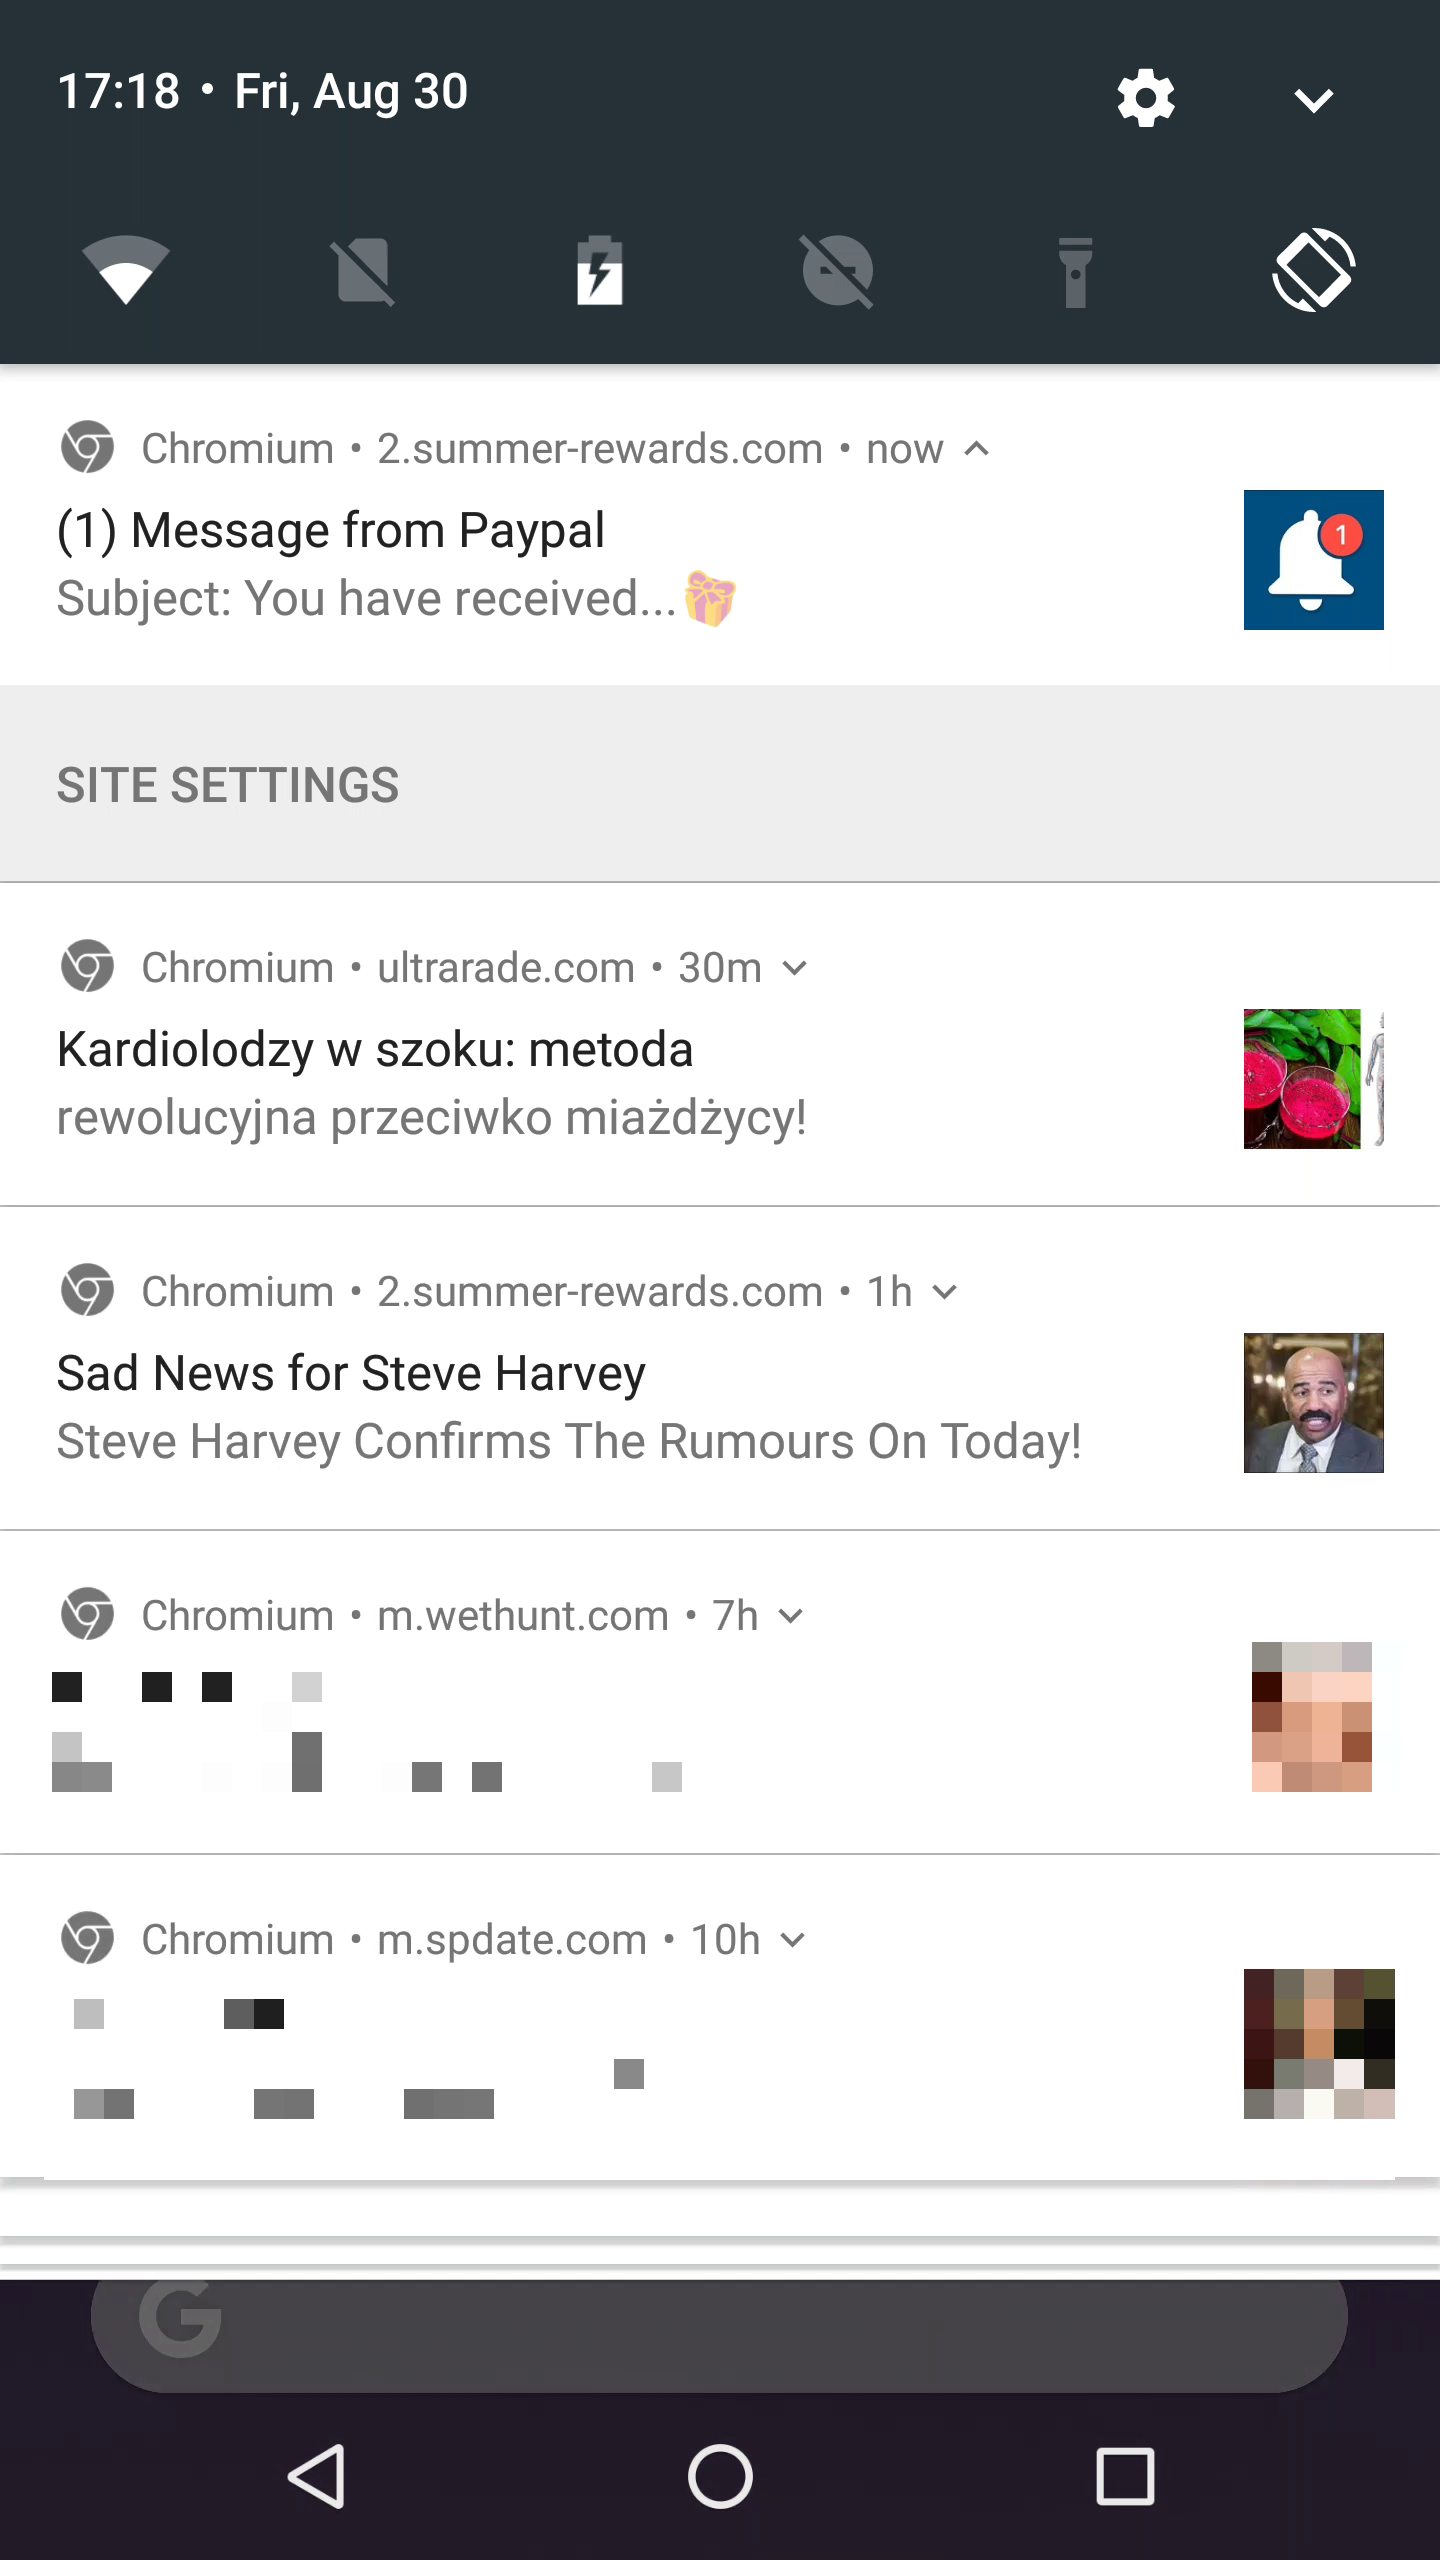
\includegraphics[width=\linewidth]{figs/mobile_disguised_1}
%         \caption{}
%     \end{center}
%     \end{subfigure}
%     \begin{subfigure}{.2\textwidth} 
%     \begin{center}
%         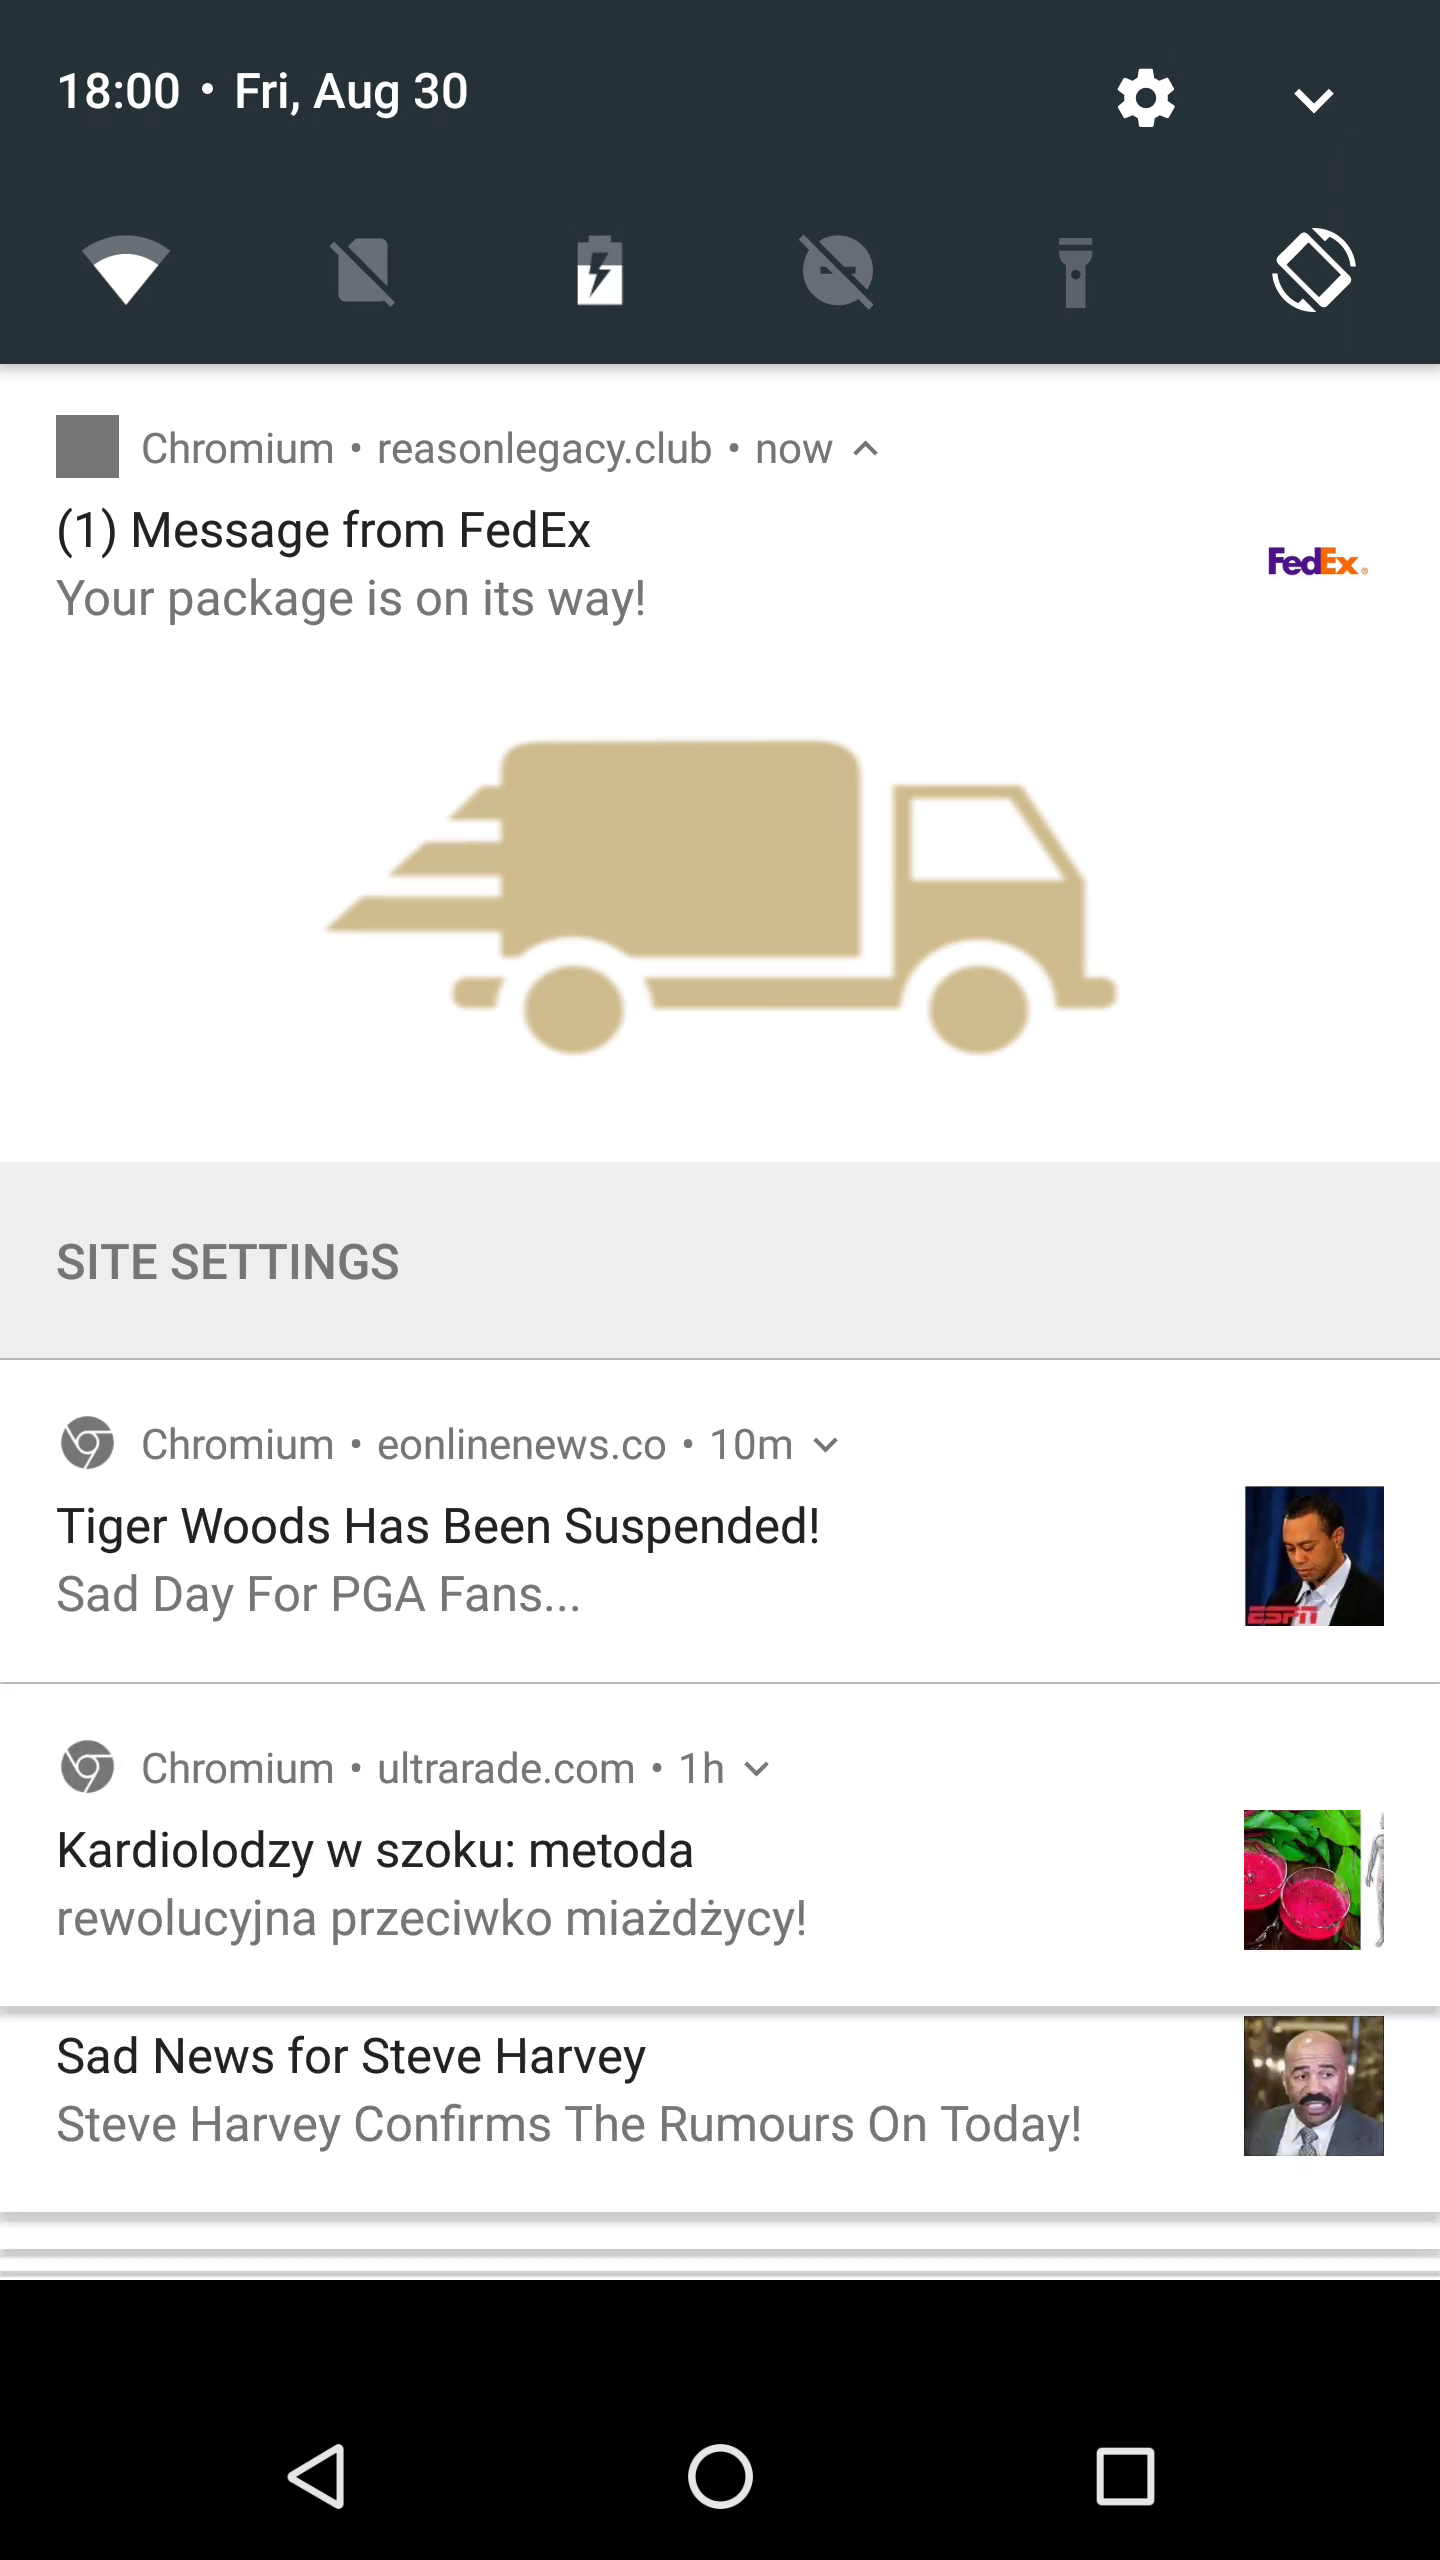
\includegraphics[width=\linewidth]{figs/mobile_disguised_2}
%         \caption{}
%     \end{center}
%     \end{subfigure}
%     \begin{subfigure}{.2\textwidth} 
%     \begin{center}
%         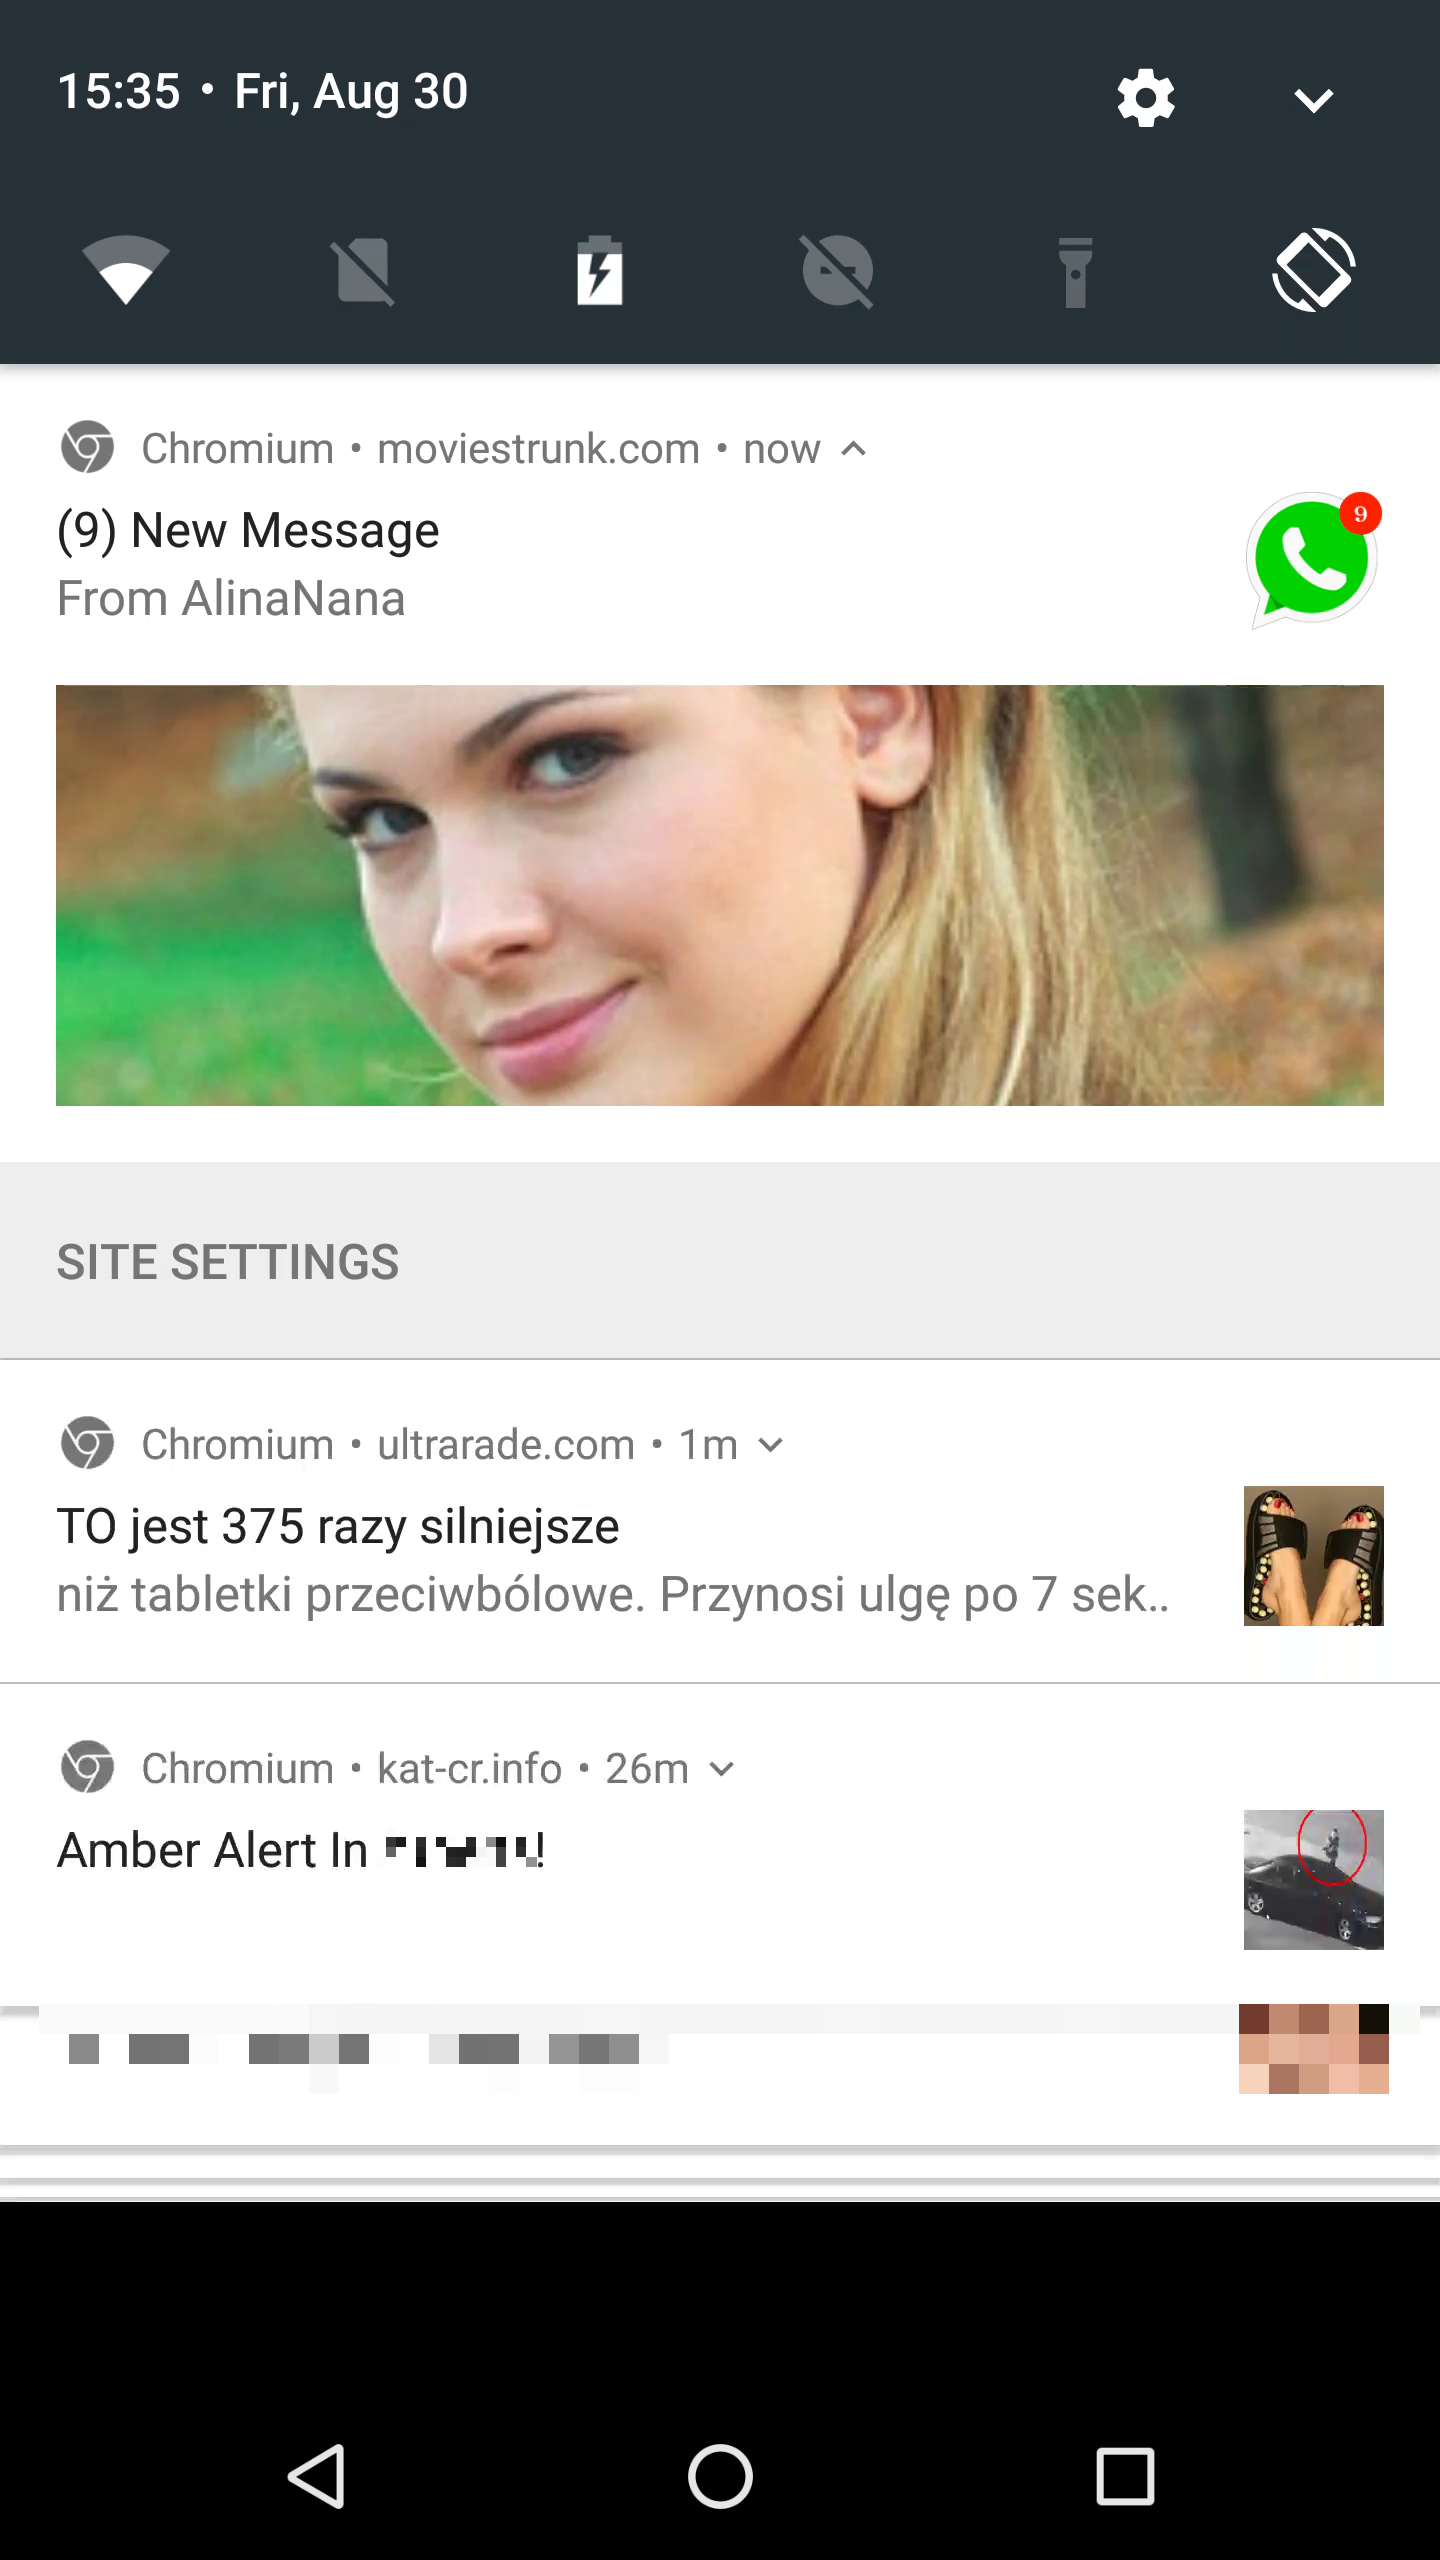
\includegraphics[width=\linewidth]{figs/mobile_disguised_3}
%         \caption{}
%         \label{fig:location}
%     \end{center}
%     \end{subfigure}
%     \caption{Title phishing: (a)Ad disguised as SMS or E-mail notification (b)Ad disguised as FedEx's application's notification (c)Ad disguised as WhatsApp's notification}
%     \label{fig:mobile_disguised_notification}
% \end{center}
% \end{figure*}

% \begin{figure}[h]
% \begin{center}
%     \begin{subfigure}{.2\textwidth}
%     \begin{center}
%         \includegraphics[width=\linewidth]{figs/mobile_phishing_2}
%         \caption{}
%         \label{mobile_phishing_2}
%     \end{center}
%     \end{subfigure}
%     \begin{subfigure}{.2\textwidth} 
%     \begin{center}
%         \includegraphics[width=\linewidth]{figs/mobile_phishing_3}
%         \caption{}
%         \label{mobile_phishing_3}
%     \end{center}
%     \end{subfigure}
%     \caption{Content phishing}
%     \label{fig:test}
% \end{center}
% \end{figure}
\section{Permission Bypassing Attack}
In this section, we demonstrate that it is possible for an adversary to  bypass requesting notification permission and successfully send push notifications to an end user.  For this attack to successfully work, we assume that attacker has control of a web page from a benign website  through exploits, phishing or other means. We will refer to the website as "benign.com" and the web page as "benign.com/attack" for further explanation. Let's say the website "benign.com" already provides push notification service to it's users (refer \ref{bypassAttack} step 1 ).If an user hasn't granted permission to "benign.com", then on visiting "bening.com/attack" page would be asked for permission as shown in step 2 of \ref{bypassAttack}. On the other hand, suppose there are users who have subscribed to notifications from "benign.com" as shown in step 3 of \ref{bypassAttack}.  In order for the adversary to take advantage of the notification permission that was already provided to the domain "benign.com", the only action required for the adversary to start sending notifications to the website's users is to register a service worker under domain "benign.com" on the users' machines. When an user visits the web page "benign.com/attack", the attacker's service worker would automatically get registered and the attacker is free to send any number of notifications to the user and all these notifications would appear to be sent by "benign.com" as shown in step 4 of \ref{bypassAttack}. In such a scenario, end user would blindly trust the notifications sent by the adversary and could be easily redirected to pages that may be used to obtain sensitive information from the user. This attack could also be used as a mean to make a website's users lose their trust in the website as they would be getting a lot of annoying or fake notifications. This attack is powerful than existing phishing attacks as even after web pages such as "benign.com/attack" is blacklisted, attacker would still be able to send notifications to the users who have already visited the page once. The only way to end the notifications would be for the user himself/herself to unregister the service worker of the attacker or revoke notification permission for the entire domain.

\begin{figure}[ht]
\caption{Demo of Bypass Notification Attack }
\begin{center}
\label{bypassAttack}
\begin{tabular}{cc}

 \begin{minipage}{.2\textwidth}
      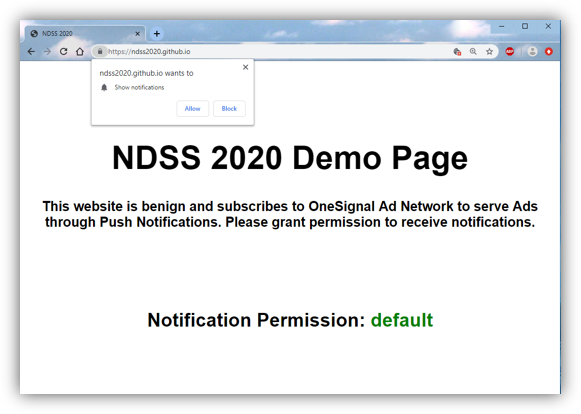
\includegraphics[width=\linewidth]{figs/attack_1.PNG}{1}
    \end{minipage}
 & 
\begin{minipage}{.2\textwidth}
      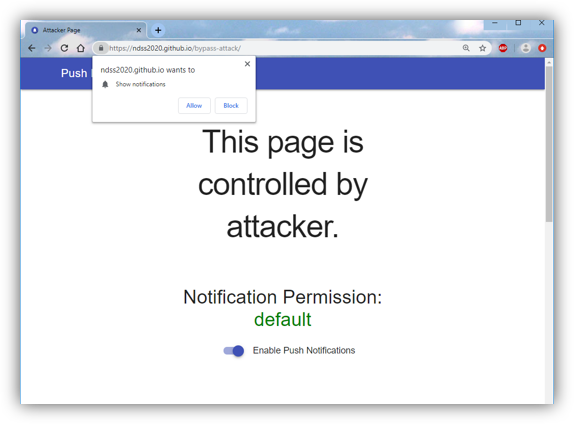
\includegraphics[width=\linewidth]{figs/attack_2.PNG}{2}
    \end{minipage}
 \\
 
\end{tabular}
      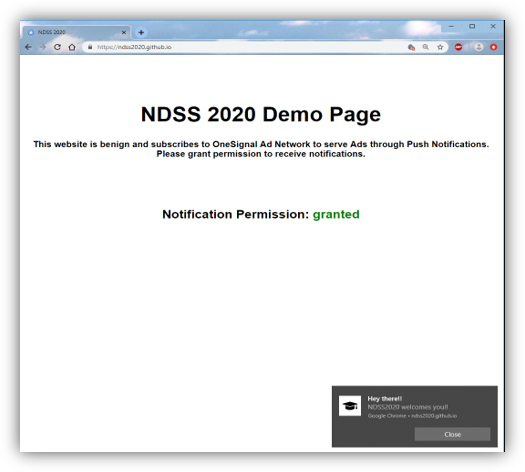
\includegraphics[width=\linewidth]{figs/attack_3.PNG}{3}
      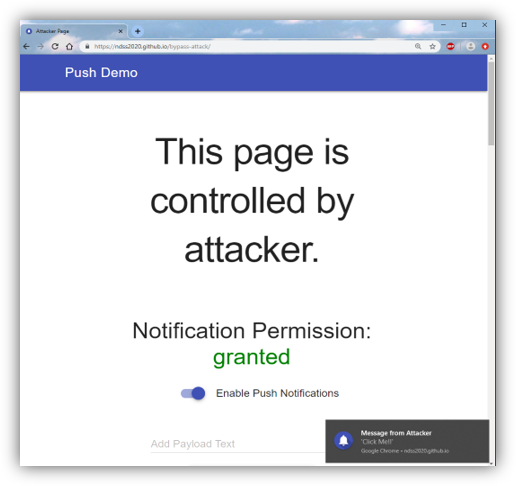
\includegraphics[width=\linewidth]{figs/attack_4.PNG}{4}
\begin{tabular}{c c}
\hline
\end{tabular}
\label{tab1}
\end{center}
\end{figure}
 

\noindent There are two main reasons for this attack to be possible. First, when an user grants permission, it is granted at the domain level and domain/website is blindly trusted. Second, any given website can register any number of service workers without user's permission as long as the multiple service workers are registered from different pages of the website. 
\section{Related Work}

%\section{Results}

Notifications Collected  could be viewed from this URL : http://172.19.48.78/info.php


\begin{figure}[h]
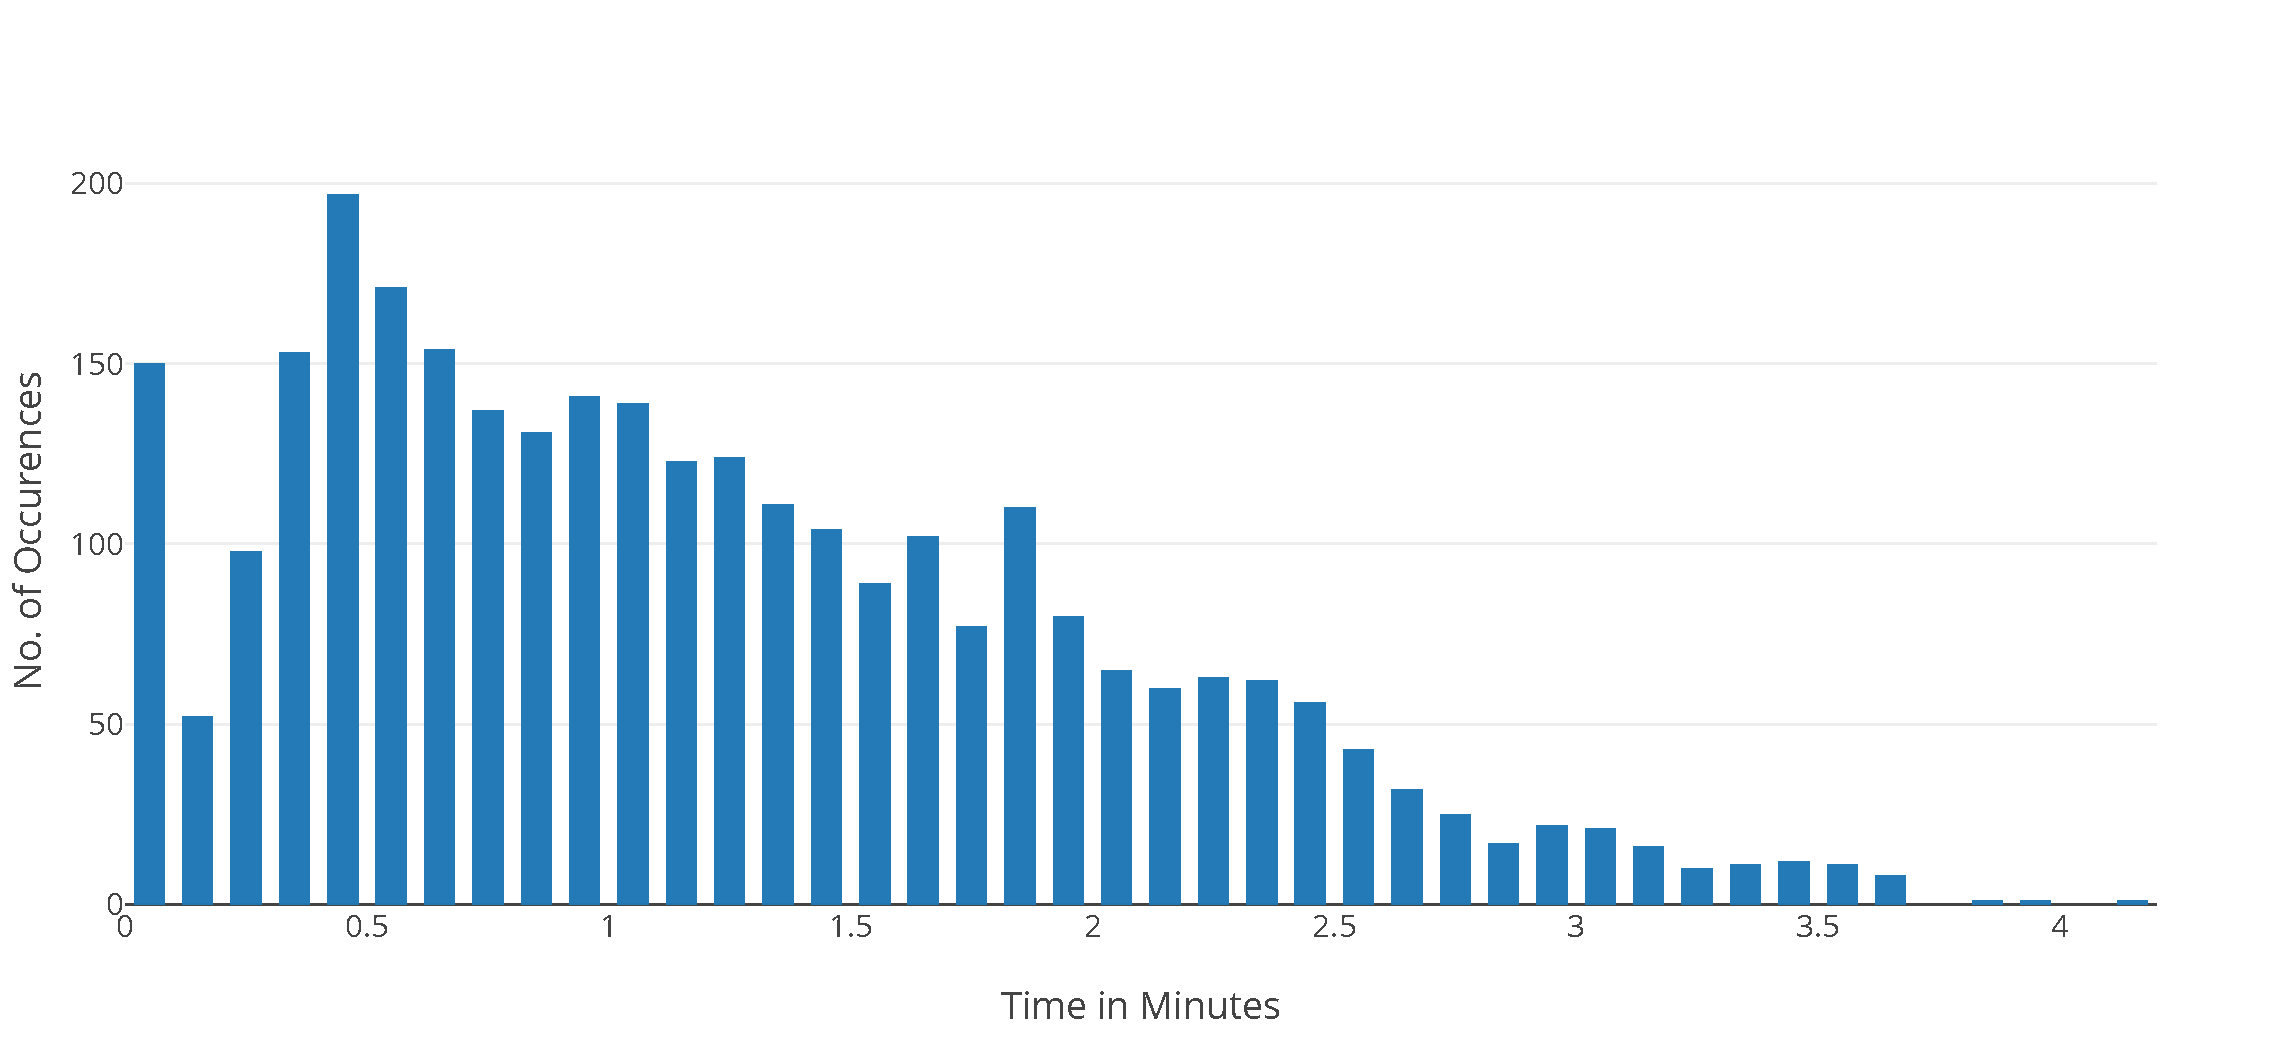
\includegraphics[width=\columnwidth]{figs/sw_reg_distribution.pdf}
\caption{Service Worker and Permission Request Time Distribution. \samuel{This graph is based on the logs collected from XXX websites}}
\label{sw_reg_time}
\end{figure}

\subsection{Observations}
\begin{itemize}
    \item Notifications collected are from different languages
    \item Suspicious notification types are "PC repair", "Payment fraud" , "Adult content"
\end{itemize}

\subsection{Steps to Identify Malicious Notifications}
\begin{itemize}
    \item Check URLs against Google Safe browsing list
    \item classify malicious URLS based on notification title and body content
\end{itemize}

"You are being Tracked ⚠️"	"Click here to protect your privacy"
\newline
"Welcome: 2500 in Bonuses"	"Claim 150 up to 500 on you five deposits."
\newline
"Amazon Secret to 1 Trillion USD!"	"Watch on Youtube Video Here!"	"https://kingofgym.com/"
\newline
"Do You Want to Win? Click Here!"	"You’ve been personally selected to take part in our 2019 Annual Visitor Survey! ..."	"https://install.pdf-maker.com/sw-loader.js"
\newline
"Use This Genius Method To Get Over 50 HD Channels In U.S."	"[Read More...]"	"https://install.incognitosearches.com/sw-loader.js"
\newline
"Hide IP, access ANY content,"	"protect browser from tracking now:..."	"https://koora-fast.com/sw.js?v=3.1.29&o=2c7ca1b72e7f4170a9e058b67498c8c7&pub=0&p=2506352&trace_id=687fef0a-c5c2-43d0-b8c6-db82e349581d"
\newline
"Fastest PDF converter"	"Free tool. No Ads. Get now>"	"https://koora-fast.com/sw.js?v=3.1.29&o=2c7ca1b72e7f4170a9e058b67498c8c7&pub=0&p=2506352&trace_id=687fef0a-c5c2-43d0-b8c6-db82e349581d"
\newline
"129022"	"Your Protection has Expired ⚠"	"Reactivate McAfee now to stay protected for y"	"https://not-robot.com/rb_serviceworker.js"
\newline
"129022"	"Mcafee License Expired Today⚠️"	"Reactivate now to stay protected for your PC"	"https://not-robot.com/rb_serviceworker.js"
\newline
"129022"	"Government Grants Available ��"	"No Payback Money Available For Funding a Business, School or Pay Off Bills!"	"https://not-robot.com/rb_serviceworker.js"
\newline
"129022"	"(5) new friend requests"		"https://not-robot.com/rb_serviceworker.js"
\newline
\newline
\newline
"Great Opportunity To Inve"	"Great Opportunity To Inve"	"https://groshi.work/swnhrj.js"
\newline
"K. (26) left you a message"	"Hi babe ..."	"https://groshi.work/swnhrj.js"
\newline
\newline
"You From Athens & Single?"	"These Russian Women Will Drive You Wild!"	"https://groshi.work/swnhrj.js"
\newline
"Drivers are furious about this"	"Drivers are furious about this"	"https://groshi.work/swnhrj.js"
\newline


Same service-worker file used by two different websites showing suspicious ads

"161540"	"Your payment info has been leaked!"	"Please fix this problem to avoid losing your deposit."	"https://klepa-i-misha.com/swnhrj.js"
"161540"	"You are being Tracked ⚠️"	"Click here to protect your privacy"	"https://klepa-i-misha.com/swnhrj.js"
"161540"	"Anna sent you (5) pictures"	"She's from Athens & waiting for you."	"https://klepa-i-misha.com/swnhrj.js"


"162148"	"Your payment info has been leaked!"	"Please fix this problem to avoid losing your deposit."	"https://notepad.ge/swnhrj.js"	"https://click.mppmnetwork.com/v2/click/"
"162148"	"Do You Like Gift Cards?"	"Take Surveys & Get Giftcards !!"	"https://notepad.ge/swnhrj.js"	"https://click.mppmnetwork.com/v2/click/"
"162148"	"You are being Tracked ⚠️"	"Click here to protect your privacy"	"https://notepad.ge/swnhrj.js"	"https://click.mppmnetwork.com/v2/click/"
"162148"	"Can CBD Really Help Back Pain?"	"Top Doctors Agree.  Prescribe CBD Oil At A Record Pace"	"https://notepad.ge/swnhrj.js"	"https://click.mppmnetwork.com/v2/click/"
"162148"	"You are being Tracked ⚠️"	"Click here to protect your privacy"	"https://notepad.ge/swnhrj.js"	"https://click.mppmnetwork.com/v2/click/"
"162148"	"Realistic 3D game"	"Realistic 3D game"	"https://notepad.ge/swnhrj.js"	"https://click.mppmnetwork.com/v2/click/"

\bibliographystyle{IEEEtranS}
\bibliography{references}
\end{document}
